% !TEX root = lfgw.tex

\chapter{Texte schreiben}
\autor{Thomas Hilarius Meyer}

Geistes- und humanwissenschaftliche Arbeiten haben besondere Anforderungen an die typografische
Gestaltung. 
Die häufigsten Anforderungen werden im folgenden der Reihe nach durchgegangen.
Manches davon ist \LaTeX-Standard; anderes wird außerhalb der Geisteswissenschaften eher
selten gebraucht.
Ein großer Bereich, für den \LaTeX{} eigentlich bekannt ist, bleibt ganz außen vor:
der Satz von komplexen mathematischen Formeln und Gleichungen.


\section{Vorüberlegungen zu typografischer Schönheit und Funktionalität}

\dictum[Louis Sullivan]{Form follows function.}

Der Grundgedanke bei der Benutzung von \LaTeX\ ist, dass sich der Autor um die inhaltliche Seite seines
Textes kümmert, und die typografische Aufbereitung den Algorithmen der Software überlässt, 
die aus der ihr mitgeteilten logischen Struktur anhand der traditionellen Regeln funktionaler Setzerkunst 
eine schön -- im Sinne funktionaler Ästhetik -- aufbereitete Druckfassung erstellt.

Dieser Ansatz widerspricht der weitverbreiteten Do-it-yourself-Mentalität der Typografie des
PC-Zeitalters, die im sehr lesenswerten Leitfaden \enquote{Erste Hilfe Typografie} der Setzer-Koryphäen
Hans Peter Willberg und Friedrich Forssmann karikiert wird:

\begin{quote}
 Das Selbermachen ist längst üblich, die Ergebnisse sind oft fragwürdig,
 weil die Laien-Typografen nicht sehen, was nicht stimmt und nicht wissen
 können, worauf es ankommt.
 So gewöhnt man sich an falsche und schlechte Typografie.
 \footcite[9]{erste_hilfe}
 \end{quote}
 
\begin{quotation}
 \emph{Du warst doch mal Sekretärin.
 Ich muss meine Diss schreiben, kannst Du mir zeigen, wie das geht?}
 
 \emph{Was} ein Doktorand oder Diplomand zu schreiben hat, das hat er studiert.
 \emph{Wie} er es zu schreiben hat, hat er nicht studiert, er setzt irgendwie drauflos.
 Mit unübersichtlicher und schlecht lesbarer Laien-Typografie schadet er oft genug seiner Arbeit.
 \footcite[86]{erste_hilfe}
\end{quotation}

Natürlich beinhaltet auch eine moderne \LaTeX -Installation keine künstliche Intelligenz mit 
vollständiger Setzerlehre und vor allem sind die Spezialanforderungen gerade an die Satzerstellung im
humanwissenschaftlichen Bereich so speziell und individuell, dass es gelegentlich nicht ohne 
\enquote{Selbermachen} und \enquote{Basteln} geht, aber dennoch ist es wichtig, sich den Grundsatz
klarzumachen: In einem \LaTeX -Dokument wird primär der \emph{Inhalt} ausgezeichnet, und erst sekundär
die Repräsentation der inhaltlichen Struktur in ein Druckbild.

Um was geht es im einzelnen beim Erstellen von Texten mit \LaTeX ? 


\section{Wahl der Dokumentklasse}

In der ersten Zeile eines \LaTeX -Dokumentes wird die Dokumentklasse des folgenden Textes 
festgelegt. Die Dokumentklasse definiert die grundsätzlichen Spielregeln:
Welche Gliederungsebenen sind vorgesehen, wie ist die grundsätzliche Formatierung aufgebaut etc.

Es existiert eine sehr große Vielzahl von verschiedenen Dokumentklassen;
so gibt es für Hausarbeiten oder Dissertationen zahlreicher Universitäten eine eigene
Dokumentklasse. Existiert eine solche, sollte man sie i.\,d.\,R. auch benutzen.

Die folgende Einführung beschränkt sich auf die Klassen des \KOMAScript-Paketes von
Markus Kohm, weil diese eine überragende typografische Qualität sowie zahllose Möglichkeiten
zur individuellen Anpassung bieten.%
\footnote{Wer allerdings ihre volle Funktionalität nutzen will, sollte sich die originale 
Dokumentation beschaffen und sich mit ihrer Hilfe genauer einarbeiten \dots}
Hinzu treten zwei Dokumentklassen für speziellere Fälle, nämlich für Präsentationen und 
Prüfungen.

\begin{labeling}{scrreprt}
 \item[scrartcl] ist die \KOMAScript-Klasse für Artikel.
 \item[scrreprt] kann gut für längere Seminar- oder auch Bachelor-Arbeiten genutzt werden.
 \item[scrbook] ist die Klasse für Bücher mit zahlreichen ausgereiften Funktionen für
  die Titelei etc.
 \item[exam] ist eine eigene Klasse zur Entwicklung von Aufgabenblättern zu Prüfungszwecken.
 \item[beamer] stellt eine ganze Reihe von Features für die Erstellung von Präsentationen
  zur Verfügung. Mit etwas Einarbeitung gelingen damit schneller bessere Präsentationen als 
  mit der verbreiteten Konkurrenz.
\end{labeling}


\minisec{Zum Unterschied zwischen \enquote{Klasse} und \enquote{Paket}}

\dictum[Goethe, Faust 1337]{Was ist mit diesem Rätselwort gemeint?}

In \LaTeX -Kreisen ebenso wie innerhalb dieser Anleitung ist häufig von \enquote{Paketen} die Rede,
die \enquote{geladen} werden müssen, um eine bestimmte Funktionalität zu gewährleisten.
Andererseits stellen zahlreiche \enquote{Klassen} bereits Features zur Verfügung etc. 
-- wie sind diese Begriffe zu verstehen?

Eine \textbf{Dokumentklasse} definiert die grundlegende Struktur zur Bearbeitung einer Textgattung
mit Hilfe von \LaTeX. Das kann ganz allgemein sein -- wie die ursprünglichen Standardklassen book, report, 
article -- oder sehr speziell -- wie die Vorlage einer Dissertation in Elektrotechnik an einer ganz
bestimmten Technischen Hochschule.

Die gewünschte Dokumentklasse wird ganz am Anfang angegeben durch das Kommando
\cs{documentclass\oarg{Optionen}\marg{NAME}}.
% sollte hier nicht deutlich gemacht werden, dass LaTeX genau dies
% auszeichnet: man muss nicht mit den atomaren Elementen aus TeX arbeiten,
% sondern nutzt eine Dokumentenklasse, die viele Detaileinstellungen vornimmt
% und darüber hinaus eine Reihe von logisch strukturierenden Voreinstellungen
% bereitstellt, die für den jeweiligen Anwendungsfall festgelegt wurden.
% Auch könnte auf die Äquivalenz zwischen Dokumentenklasse und Vorlagen bei 
% Textverarbeitungssystemen hingewiesen werden.

Grundsätzlich gilt: Je spezieller eine Dokumentklasse ist, desto genauer passt sie zu einer spezifischen
Aufgabenstellung und desto eher wird sie spezifische Sonderanforderungen befriedigen -- bis hin zur
Integration des Universitätslogos etc.
Je allgemeiner eine Klasse ist, desto eher wird man bei Spezialbedürfnissen darauf angewiesen sein,
diese auf anderem Wege zu implementieren.
Jetzt kommen die Pakete ins Spiel:

\textbf{Pakete} erweitern die Funktionalität einer %beliebigen
Dokumentklasse um einzelne, meist
thematisch zusammenhängende Funktionen. Beispiele sind etwa die Möglichkeit zur Einbindung von
Grafiken, die Erstellung von Registern, bessere Möglichkeiten zur Erstellung von komplexen Tabellen etc.
Die meisten in dieser Anleitung vorgestellten Möglichkeiten basieren auf besonderen Paketen, die
oftmals von und für Geisteswissenschaftler[n] entwickelt wurden.

Das \enquote{Laden} eines Paketes erfolgt durch den Befehl \cs{usepackage}\oarg{Optionen} \marg{PAKETNAME}

Dokumentklassen und Pakete enthalten in der Regel eine ziemlich gute Dokumentation, die man
ggf. zu Rate ziehen sollte, um ihren vollen Funktionsumfang ausnutzen zu können.%
\footnote{Wie kann man die Paketdokumentation aufrufen? 
    Vgl. hierzu \ref{paketdoku} auf S.~\pageref{paketdoku} }


\section{Nationale Besonderheiten -- das Paket babel}
\label{babel}

\dictum[Gen 11,7]{Wohlan, lasst uns hinabfahren und daselbst ihre Sprache verwirren, dass keiner mehr 
    des anderen Sprache verstehe.}

Das vielleicht wichtigste Paket, das in praktisch jedem Dokument zu laden ist, heißt \paket{babel}.
Es sorgt dafür, dass \LaTeX\ an die verschiedenen nationalsprachlichen Besonderheiten angepasst wird.
Das betrifft auch automatisch eingesetzte Begriffe wie \enquote{Kapitel} statt \enquote{chapter} sowie
sprachspezifische typografische Regelungen.

Der Aufruf des Paketes \paket{babel} erfolgt wie bei allen Paketen: 
% Ich würde nicht von Aufruf, sondern von Bereitstellen der Funktionalität sprechen
\cs{usepackage\oarg{Liste mit benutzen Sprachen}\marg{babel}}
Die in der Liste zuletzt angegebene Sprache ist die Standardsprache des Dokuments. 
%(die am Anfang eingestellt ist) dar.

Babel unterstützt eine ganze Reihe von Sprachen; für Geisteswissenschaftler am wichtigsten sind
wohl:

\begin{labeling}{polutonikogreek}
 \item[german] Deutsch, alte Rechtschreibung (1901)
 \item[ngerman] Deutsch gemäß der Rechtschreibreform von 1996
 \item[greek] Neugriechisch (nur Akut, keine \emph{spiritus}, wahrscheinlich auch kein \emph{Iota subscriptum})
%von Philipp angepaßt, war vorher:
% \item[polutonikogreek] (XXX was ist der Unterschied)
 \item[greek.ancient] oder \ldots 
 \item[polutonikogreek] Altgriechisch (Akut, Gravis, Zirkumflex; spiritus lenis und asper; Iota subscriptum)
\end{labeling}


Auch der Dokumentklasse sollte man die Standardsprache des Dokumentes bekanntgeben.
Denn zahlreiche Pakete, die später geladen werden, werten diese Sprachoption aus und 
passen sich an (z.\,B. \paket{varioref}).
% Ausdruck ist anthropomorphisierend -- nicht passen sich an, sondern 
% passen sprachsensible Konstruktionen an

Somit ergibt sich folgender typischer Dokumentbeginn:

\begin{lfgwcode}{label={lis:dokumentbeginn}}
 \documentclass[ngerman]{scrreprt}
 \usepackage[polutonikogreek,ngerman]{babel}
\end{lfgwcode}

(Wenn keine griechischen Einschübe benutzt werden, kann die Angabe von \lstinline/polutonikogreek/
%natürlich wegbleiben.)
entfallen.)

\minisec{Wechsel zu einer anderen Sprache}

Im laufenden Dokument kann auf eine der im Paketaufruf angegebenen Sprachen umgeschaltet werden:

\begin{lfgwcode}{label={lis:sprachumschaltung}}
 \selectlanguage{polutonikogreek}
\end{lfgwcode}


%\minisec{Alternative: Das Paket \paket{polyglossia}}
%
%\paket{polyglossia}


\section{Seitengestaltung und Seitenspiegel}
\label{komaskript}
\index{Seitenspiegel} \index{Goldener Schnitt}

Die folgenden Angaben sind nur von Interesse, wenn man als Papierformat nicht DIN"~A4-Papier 
nutzen will und/oder nicht die eingebauten Satzspiegelkonstruktionen verwenden kann.
In den allermeisten Fällen empfiehlt es sich, den Vorgaben insbesondere der Dokumentklassen von
\KOMAScript{} zu überlassen, wie das Verhältnis von bedrucktem Bereich und Rändern aufzuteilen ist,
da der Klassenautor Markus Kohm sehr viel Aufwand in die Definition des Satzspiegels gesteckt hat und
klassische Ideale wie den Goldenen Schnitt berücksichtigt.

Dazu reicht es, bei der Angabe der Dokumentklasse das Papierformat als Option \lstinline/paper=.../ anzugeben.
Vordefiniert sind: letter, legal, executive, a0, a1, a2, a3, a4, a5, a6, a7, a8, b0 bis b8, c0 bis c8 und
d0 bis d8. 
% statt 
% a0, a1, a2, a3, a4, a5, a6, a7, a8
% besser: a0 bis a8
%

Außerdem ist es möglich, die Breite und Höhe des Papiers direkt anzugeben:
\lstinline/paper=200mm:200mm/.

Lediglich, wenn z.\,B. spezielle Vorgaben des Verlages es erforderlich machen, empfiehlt es sich
die Einstellungen der Seitenränder sowie ihrer zahlreichen Bestandteile (Marginalspalten, Bereiche
für Fußnoten und Seitenzahlen, Kolumnentitel usw.) direkt zu verändern.
 

\minisec{Direktes Einstellen des Papierformats und Satzspiegels}

Dies lässt sich am einfachsten mit Hilfe des Paketes \paket{geometry} von Hideo Umeki erreichen.
Mit seiner Hilfe ist es problemlos möglich, besondere Wünsche des Verlages hinsichtlich der Satzspiegelgestaltung zu erfüllen. Das Paket übergibt dem Nutzer die volle Kontrolle über die
Randeinstellungen -- überlässt ihm aber auch die ganze Verantwortung in ästhetischer Hinsicht.

\minisec{Beschnittmarken}
\index{Beschnittmarken}

Wenn man eine Druckvorlage für ein besonders Papierformat erzeugt, aber seine Korrekturausdrucke
auf üblichen DIN"~A4-Papier erstellt, kann man sich die \enquote{wirklichen} Größenverhältnisse von
Textblöcken und Rändern oft nicht gut vorstellen.

Hier hilft das Paket \paket{crop}, das Randmarkierungen, Beschnittmarken, in verschiedener
Ausprägung erzeugt, wie sie auch von manchen Buchbindereien gewünscht werden, um den Buchblock
präzise auf das endgültige Maß zuschneiden zu können.


\minisec{Ein- oder zweiseitiges Layout}

Bei der Einstellung der Dokumentklasse kann durch die Optionen \opt{oneside} bzw.
\opt{twoside} ein- bzw. zweiseitiges Layout verlangt werden.

Beim einseitigen Layout sind alle Seiten gleich gestaltet, während beim zweiseitigen Layout zwischen
linken und rechten Seiten unterschieden wird. Definitionsgemäß haben \enquote{linke} Seiten gerade
Seitenzahlen und \enquote{rechte} Seiten ungerade.

Die Unterscheidung hat z.\,B. auf die Positionierung der Seitenzahlen (mittig oder außen), 
Kolumnentitel und Marginalien Einfluss.


\section{Textgliederung}

\minisec{Automatischer Zeilenumbruch und Absatzwechsel}

\TeX\ führt den Zeilenumbruch automatisch durch.

Die Absatzgrenze wird durch eine Leerzeile markiert. 

Alternativ kann durch \lstinline/\\/ ein Zeilenwechsel erzwungen werden.%
\footnote{Ganz so einfach ist es nicht.}
% Wieso nicht?
% Entweder erklären oder löschen.

\minisec{Gliederung durch Zwischenüberschriften}

\begin{lfgwcode}{}
 \begin{document}
 \part{Ein Teil des Teils}
 \chapter{Ein Kapitel}
 \section{Ein Abschnitt}
 \subsection{Ein Unterabschnitt}
 \subsubsection{Ein kleiner Unterabschnitt}
 
 \chapter*{Ein Kapitel ohne Eintrag im Inhaltsverzeichnis}
 \section*{Ein Abschnitt ohne Eintrag im Inhaltsverz.}
 \subsection*{Ein Unterabs. o. E. im Iv.}
 \subsubsection*{Ein kleiner Unterabschnitt o.\,E.i.\,I.}
 
 \chapter[Kurzfssg. f. d. Kolumnentitel]{Ein Kapitel}
 \section[Kurzfssg. f. d. Kolumnentitel]{Ein Abschnitt}
 \subsection[Kurzfssg. f. d. Kolumnentitel]{Ein Unterabschnitt}
 
 \end{document}
\end{lfgwcode}

Texte lassen sich in \LaTeX{} mit Hilfe eines hierarchischen Systems von Überschriften gliedern:

\begin{labeling}{Hummel}
 \item[2-6] Texte der Kategorien 
    \lstinline/book/, 
    \lstinline/scrbook/, 
    \lstinline/report/ und 
    \lstinline/scrreprt/ 
 bestehen aus Teilen (\lstinline/\part{}/)
 \footnote{Ehrlich gesagt: eher selten. 
 \lstinline/part/ 
 erzeugt einen \enquote{Zwischentitel},
 der im deutschsprachigen Raum eher unüblich ist. Ausprobieren! }
 und Kapitel (\lstinline/\chapter/);
 desweiteren lassen sich alle Texte in Abschnitte und Unterabschnitte untergliedern 
 (\lstinline/\section{}/ bis \lstinline/\subsubsection{}/) 
 gliedern.
 Jede Überschrift beeinflusst die Kolumnentitel (s.\,u.) und erzeugt automatisch einen Eintrag
 im Inhaltsverzeichnis.
 
 \item[8-11] Die \enquote{Sternvarianten} der Gliederungsbefehle erzeugen die gleiche
 Formatierung der Überschriften, hinterlassen aber keinen Eintrag im Inhaltsverzeichnis.
 Außerdem werden die Überschriften nicht nummeriert.
 
 \item[13-15] Die Kapitel und ggf. Abschnittsüberschriften werden auch als lebende Kolumnentitel
 verwendet. Wenn sie dafür zu lang sind, kann man in eckigen Klammern einen alternativen
 Kurztitel zur Verwendung als Kolumnentitel angeben. \index{Kolumnentitel}
\end{labeling}



\section{Schriftauszeichnungen}
\index{Auszeichnungsschriften}

\dictum[Mies van der Rohe]{Weniger ist mehr.}

Innerhalb gedruckter Texte lassen sich auf drei Weisen verschiedene Passagen typografisch voneinander
absetzen:
durch eine Veränderung des Schriftschnittes,
der Schriftgröße und
der Schriftart.

\subsection{Auszeichnung über Schriftschnitt}
\index{Schriftschnitt}
\index{kursiv}
\index{Kapitälchen}
\index{fett}
\index{Unterstreichung}

Standardmäßig erlaubt \LaTeX\ die typischen Auszeichnungen:

\begin{center}
\begin{tabular}{lll}
      Befehl                &       Beschreibung                        & typograf. Bewertung \\
      \hline
 \lstinline/\emph{}/        &   \emph{hervorgehoben} (z.\,B. kursiv in recte-Texten)        &   $+$ \\
 \lstinline/\textit{}/      &       \textsl{kursiv}                     &   $--$\\
 \lstinline/\textsl{}/      &       \textsl{schräggestellt}             &   $--$\\
 \lstinline/\textsc{}/      &       \textsc{Kapitälchen}                &   $+$ \\
 \lstinline/\textbf{}/      &       \textbf{fett}                       &   $+/-$ \\
 \lstinline/\underline{}/   &       \underline{unterstrichen}           &   $-$ \\
 \lstinline/\texttt{}/      &       \texttt{Schreibmaschinenschrift}    &   ? \\
 \lstinline/\textsuperscript{}/ &   Text\textsuperscript{hochgestellt}  &     \\
 \lstinline/\textsubscript{}/ &     Text\textsubscript{tiefgestellt}    &     \\
 \end{tabular} 
\end{center}

\minisec{Unterstreichungen}

In der anspruchsvolleren Typografie gelten Unterstreichungen als verpöntes Überbleibsel
aus der Schreibmaschinenzeit. Im klassischen Bleisatz wurde nicht mit Unterstreichungen
gearbeitet.

Dennoch können Unterstreichungen in Sonderfällen sinnvoll sein.

Oftmals wünscht man sich dann sogar eine größere Auswahl an verschiedenen 
Unterstreichungsarten, um etwa verschiedene Textherkünfte o.\,ä. markieren zu können.

Abhilfe schafft das Paket \paket{ulem}, das verschiedene Arten der Unterstreichung
ermöglicht:

\begin{center}
  \begin{tabular}{ll}
      Befehl &      Beschreibung \\
      \hline
      \lstinline/\uline{text}/ &    \uline{einfaches Unterstreichen} \\
      \lstinline/\uuline{text}/ &   \uuline{doppeltes Unterstreichen}\\
      \lstinline/\uwave{text}/ &    \uwave{wellenförmiges Unterstreichen}\\
      \lstinline/\sout{text}/ &     \sout{Durchstreichen} \\
      \lstinline/\xout{text}/ &     \xout{Ausschraffieren von Text} \\
  \end{tabular}    
\end{center} 


\minisec{Texte sperren}

Eine sehr elegant-konservative typografische Möglichkeit zur aktiven Auszeichnung ist das 
\textls{Sperren}  
von Textpassagen. Hierzu stellt das Paket \paket{microtype} den Befehl
\lstinline/\textls{Text}/ zur Verfügung.
% Das ist jetzt nicht Ernst gemeint.
% "A man who would letterspace lower case would steal sheep" Frederic Goudy

\subsection{Veränderung der Schriftgröße}
\index{Schriftgröße}

Die Schriftgröße lässt sich sehr leicht verändern, wobei anzumerken ist, dass
die konkrete Bedeutung der Größenangaben von der Dokumentklasse vorgenommen werden:

\begin{center} 
\begin{tabular}{ll}
          Befehl &      Beschreibung \\
          \hline
 \lstinline/\Huge{}/        &   \Huge{\strut Riesig!} \\
 \lstinline/\huge{}/        &   \Huge{\strut riesig} \\
 \lstinline/\LARGE{}/       &   \LARGE{\strut sehr, sehr groß} \\
 \lstinline/\Large{}/       &   \Large{\strut sehr groß} \\
 \lstinline/\large{}/       &   \large{\strut groß} \\
 \lstinline/\normalsize{}/  &   \normalsize{normal groß (Grundschriftgröße)} \\
 \lstinline/\small{}/       &   \small{klein} \\
 \lstinline/\footnotesize{}/    &   \footnotesize{so groß wie die Fußnoten} \\
 \lstinline/\scriptsize{}/  &   \scriptsize{für Kleingedrucktes} \\
 \lstinline/\tiny{}/        &   \tiny{wirklich winzig} \\
\end{tabular}
\end{center}

\subsection{Verschiedene Schriftarten}

\minisec{Normale Schriften}
\label{sec:normale-schriften}

In den 90er Jahren konnte man ein \LaTeX-Dokument sofort an der Schrift erkennen.
Die meisten Dokumente wurden in der \TeX-Schrift \texttt{Computer Modern Roman} erstellt.
Man konnte auch andere Schriften installieren, das war aber mit einigem Aufwand verbunden.

Dank \LuaLaTeX{} ist es heutzutage möglich beliebige TrueType oder OpenType Schriften zu benutzen.
Gleichzeitig nahm die Zahl der qualitativ hochwertigen freien Schriften zu.
Viele dieser Schriften sind Bestandteil von \TeXLive{} und können so ohne Aufwand benutzt werden.

Ein weiterer Vorteil der OpenType Schriften ist die Verwendung von erweiterten Attributen, 
so lassen sich z.\,B. unterschiedliche Ziffern auswählen.

\newfontfamily\LIMOfont[Ligatures=TeX,Numbers={Monospaced,OldStyle}]{Linux Libertine O}
\newfontfamily\LIVOfont[Ligatures=TeX,Numbers={Proportional,OldStyle}]{Linux Libertine O}
\newfontfamily\LIMLfont[Ligatures=TeX,Numbers={Monospaced,Lining}]{Linux Libertine O}
\newfontfamily\LIVLfont[Ligatures=TeX,Numbers={Proportional,Lining}]{Linux Libertine O}

  \begin{tabular}{ll}
    {\LIMOfont 0123456789} &\verb+Numbers={Monospaced,OldStyle}+\\
    {\LIMLfont 0123456789} &\verb+Numbers={Monospaced,Lining}+\\
    {\LIVOfont 0123456789} &\verb+Numbers={Proportional,OldStyle}+\\
    {\LIVLfont 0123456789} &\verb+Numbers={Proportional,Lining}+
  \end{tabular}

\LuaLaTeX{} kennt drei verschiedene Schriften, siehe Beispiel~\ref{lst:luatex-schriften}.
Diese werde von \LaTeX{} für die entsprechenden Befehle benutzt.
Der Befehl \cs{setsansfont} definiert die Schrift für \cs{textsf},
\cs{setmonofont} die Schrift für \cs{texttt} und \cs{setromanfont} die normale Textschrift.

Die Option \texttt{[Ligature=TeX]} aktiviert ein paar Ligaturen, 
die die Eingabe von Text erleichtern und bei den Standard \LaTeX{}-Schriften ebenfalls definiert waren.
Aus der Eingabe \verb+--+ wird ein \enquote{--}, aus der Eingabe \verb+---+ wird ein \enquote{---}.
Diese Definition sorgt manchmal für Überraschungen, 
da auch \verb+!`+ zu \enquote{!`} und \verb+?`+ zu \enquote{?`} gewandelt wird.
Gibt man den Text direkt in Unicode ein, kann man auf die Ligaturen verzichten.
In vielen alten Texten werden sie jedoch verwendet, daher diese Option.

Außerdem ist es möglich zusätzliche Schriftfamilien zu definieren, 
diese können dann für andere Sprachen benutzt werden, 
wenn die Hauptschrift nicht über die benötigten Zeichen verfügt.
Oder man definiert für Tabellen eine eigene Schrift, 
damit alle Ziffern die gleiche Breite haben. 

\begin{lfgwcode}{label={lst:luatex-schriften}}
  % !TEX TS-program = LuaLaTeX
  % !TEX encoding = UTF-8
  \setromanfont[Ligatures=TeX]{Linux Libertine}
  \setsansfont[Ligatures=TeX]{Linux Libertine}
  \setmonofont[Ligatures=TeX]{Linux Libertine}
  \newfontfamily\LITABfont[Ligatures=TeX,Numbers={Monospaced,Lining}]{Linux Libertine}
\end{lfgwcode}

Benötigt man nur eine Schrift, weil es z.\,B. keine kursive oder fette Variante der Schrift gibt,
so reicht der \cs{newfonface}-Befehl.
Für arabische, hebräische oder chinesische Schriften gibt es normalerweise nur eine Variante.
Gleiches gilt für Symbolschriften wir im Beispiel \ref{lst:luatex-schriften-einzel}.
In diesem Fall wäre es aber besser gewesen, das \paket{fontawesome} Paket zu verwenden, 
mit diesem kann man die Symbole mit ihrem Namen ansprechen.

\begin{lfgwcode}{label={lst:luatex-schriften-einzel}}
  % !TEX TS-program = LuaLaTeX
  % !TEX encoding = UTF-8
  \newfontface\AWsome{FontAwesome}
  % besser, funktioniert auch mit pdfLaTeX:
  \usepackage{fontawesome}  
\end{lfgwcode}

Für viele der hier vorgestellten Schriften gibt es auch \LaTeX-Pakete, 
die die Verwendung mit \pdfLaTeX{} ermöglichen (siehe \ref{lst:pdflatex-schriften}). 
Dann stehen aber weniger Optionen zur Verfügung.
So fehlen z.\,B. die nichtlateinischen Buchstaben und es gibt nur eine Art Ziffern.

\begin{lfgwcode}{label={lst:pdflatex-schriften}}
  \usepackage{libertine}
\end{lfgwcode}


\minisec{Die \TeX-User-Group-Schriften}

Verschiedene \TeX-User-Gruppen haben sich zusammengetan um die Weiterentwicklung der 
\texttt{Computer Modern Roman} zur \texttt{Latin Modern Roman} zu finanzieren.
Diese Schrift sollte alle Lateinischen Schriftzeichen und Akzente umfassen und 
somit auch für komplizierte Schriften wie Vietnamesisch geeignet sein.

Nach dem Erfolg dieser Erweiterung wurden dann auch die klassischen PostScript-Schriften überarbeitet.
Da die Namen rechtlich geschützt sind, wurden ähnlich klingende Namen gewählt,
die mit etwas Fantasie den Rückschluss auf die Originalnamen zulassen.
Diese Schriften wurden in der \texttt{TeX Gyre} Familie zusammengefasst.

Im Jahre 2007 wurde von Microsoft \Program{Office 2007} eingeführt und damit eine 
Kodierung für mathematische Zeichensätze definiert.
In der Folge entstand ein Mathematikzeichensatz für \texttt{Latin Modern Roman} sowie etwas später 
entsprechende Zeichensätze für die weiteren Schriften.

\newfontfamily\LMRfont[Ligatures=TeX,Numbers={Proportional,OldStyle}]{Latin Modern Roman}
\newfontfamily\ADfont[Ligatures=TeX,Numbers={Proportional,OldStyle}]{TeX Gyre Adventor}
\newfontfamily\BOfont[Ligatures=TeX,Numbers={Proportional,OldStyle}]{TeX Gyre Bonum}
\newfontfamily\CHfont[Ligatures=TeX,Numbers={Proportional,OldStyle}]{TeX Gyre Chorus}
\newfontfamily\CUfont[Ligatures=TeX,Numbers={Proportional,OldStyle}]{TeX Gyre Cursor}
\newfontfamily\HEfont[Ligatures=TeX,Numbers={Proportional,OldStyle}]{TeX Gyre Heros}
\newfontfamily\PAfont[Ligatures=TeX,Numbers={Proportional,OldStyle}]{TeX Gyre Pagella}
\newfontfamily\SCfont[Ligatures=TeX,Numbers={Proportional,OldStyle}]{TeX Gyre Schola}
\newfontfamily\TEfont[Ligatures=TeX,Numbers={Proportional,OldStyle}]{TeX Gyre Termes}

\begin{tabular}{llll}
Schriftname & Buchstaben & Textziffern \\\hline
\LMRfont Latin Modern Roman &\LMRfont abcdef ABCDEF &\LMRfont 1234567890 \\
\ADfont TeX Gyre Adventor   &\ADfont abcdef ABCDEF  &\ADfont 1234567890 \\
\BOfont TeX Gyre Bonum      &\BOfont abcdef ABCDEF  &\BOfont 1234567890 \\
\CHfont TeX Gyre Chorus     &\CHfont abcdef ABCDEF  &\CHfont 1234567890 \\
\CUfont TeX Gyre Cursor     &\CUfont abcdef ABCDEF  &\CUfont 1234567890 \\
\HEfont TeX Gyre Heros      &\HEfont abcdef ABCDEF  &\HEfont 1234567890 \\
\PAfont TeX Gyre Pagella    &\PAfont abcdef ABCDEF  &\PAfont 1234567890 \\
\SCfont TeX Gyre Schola     &\SCfont abcdef ABCDEF  &\SCfont 1234567890 \\
\TEfont TeX Gyre Termes     &\TEfont abcdef ABCDEF  &\TEfont 1234567890 \\
\end{tabular} 

\minisec{Weitere \TeXLive-Schriften}

\TeXLive{} bringt bereits eine große Auswahl an Schriften mit.
Der Unterbaum \texttt{fonts} ist mit knapp 2~GigaByte das zweitgrößte Verzeichnis.
Hier lohnt sich der Blick in die Unterverzeichnisse \texttt{truetype} und \texttt{opentype}.
 
\newfontfamily\LLfont[Ligatures=TeX,Scale=0.9,Numbers={Proportional,OldStyle}]{Linux Libertine O}
\newfontfamily\LBfont[Ligatures=TeX,Scale=0.9,Numbers={Proportional,OldStyle}]{Linux Biolinum O}
\newfontfamily\OSfont[Ligatures=TeX,Scale=0.9,Numbers={Proportional,OldStyle}]{Old Standard}
\newfontfamily\APfont[Ligatures=TeX,Scale=0.9,Numbers={Proportional,OldStyle}]{Antykwa Poltawskiego}
\newfontfamily\ATfont[Ligatures=TeX,Scale=0.9,Numbers={Proportional,OldStyle}]{Antykwa Torunska}
\newfontfamily\FSEfont[Ligatures=TeX,Scale=0.9,Numbers={Proportional,OldStyle}]{FreeSerif}
\newfontfamily\FSAfont[Ligatures=TeX,Scale=0.9,Numbers={Proportional,OldStyle}]{FreeSans}   
\newfontfamily\FMfont[Ligatures=TeX,Scale=0.9,Numbers={Proportional,OldStyle}]{FreeMono}
\newfontfamily\PSEfont[Ligatures=TeX,Scale=0.9,Numbers={Proportional,OldStyle}]{PT Serif}
\newfontfamily\PSAfont[Ligatures=TeX,Scale=0.9,Numbers={Proportional,OldStyle}]{PT Sans}    
\newfontfamily\PMfont[Ligatures=TeX,Scale=0.9,Numbers={Proportional,OldStyle}]{PT Mono}
\newfontfamily\DVSEfont[Ligatures=TeX,Scale=0.8,Numbers={Proportional,OldStyle}]{DejaVu Serif}
\newfontfamily\DVSAfont[Ligatures=TeX,Scale=0.8,Numbers={Proportional,OldStyle}]{DejaVu Sans}
\newfontfamily\DVSMfont[Ligatures=TeX,Scale=0.8,Numbers={Proportional,OldStyle}]{DejaVu Sans Mono}
\newfontfamily\Junicodefont[Ligatures=TeX,Scale=0.9,Numbers={Proportional,OldStyle}]{Junicode}
\newfontfamily\Gentiumfont[Ligatures=TeX,Scale=0.9,Numbers={Proportional,OldStyle}]{Gentium Basic}
\newfontfamily\NotoSAfont[Ligatures=TeX,Scale=0.9,Numbers={Proportional,OldStyle}]{NotoSans}
\newfontfamily\NotoSEfont[Ligatures=TeX,Scale=0.9,Numbers={Proportional,OldStyle}]{NotoSerif}
%\newfontfamily\NotoMOfont[Ligatures=TeX,Scale=0.9,Numbers={Proportional,OldStyle}]{NotoMono} % TL 2018
%\newfontfamily\NotoMOfont[Ligatures=TeX,Scale=0.9,Numbers={Proportional,OldStyle}]{NotoSansMono} %% TL 2019

\noindent
\begin{tabular}{lllll}
Schriftname                 & Buchstaben & Griechisch & Kyrillisch & Textziffern \\\hline
\LLfont Linux Libertine O   &\LLfont abce ABCD     &\LLfont αβγδΑΒΓ    &\LLfont абвгдАБВГ   &\LLfont 1234567890 \\
\LBfont Linux Biolinum O    &\LBfont abce ABCD     &\LBfont αβγδΑΒΓ    &\LBfont абвгдАБВГ   &\LBfont 1234567890 \\
\OSfont Old Standard        &\OSfont abce ABCD     &\OSfont αβγδΑΒΓ    &\OSfont абвгдАБВГ   &\OSfont 1234567890 \\
\ATfont Antykwa Torunska    &\ATfont abce ABCD     &\ATfont αβγδΑΒΓ    &\ATfont абвгдАБВГ   &\ATfont 1234567890 \\
\FSEfont FreeSerif          &\FSEfont abce ABCD    &\FSEfont αβγδΑΒΓ   &\FSEfont абвгдАБВГ  &\FSEfont 1234567890 \\
\FSAfont FreeSans           &\FSAfont abce ABCD    &\FSAfont αβγδΑΒΓ   &\FSAfont абвгдАБВГ  &\FSAfont 1234567890 \\
\FMfont FreeMono            &\FMfont abce ABCD     &\FMfont αβγδΑΒΓ    &\FMfont абвгдАБВГ   &\FMfont 1234567890 \\
\DVSEfont DejaVu Serif      &\DVSEfont abce ABCD   &\DVSEfont αβγδΑΒΓ  &\DVSEfont абвгдАБВГ &\DVSEfont 1234567890 \\
\DVSAfont DejaVu Sans       &\DVSAfont abce ABCD   &\DVSAfont αβγδΑΒΓ  &\DVSAfont абвгдАБВГ &\DVSAfont 1234567890 \\
\DVSMfont DejaVu Sans Mono  &\DVSMfont abce ABCD   &\DVSMfont αβγδΑΒΓ  &\DVSMfont абвгдАБВГ &\DVSMfont 1234567890 \\
\NotoSEfont Noto Serif      &\NotoSEfont abce ABCD &\NotoSEfont αβγδΑΒΓ    &\NotoSEfont абвгдАБВГ &\NotoSEfont 1234567890 \\
\NotoSAfont Noto Sans       &\NotoSAfont abce ABCD &\NotoSAfont αβγδΑΒΓ    &\NotoSAfont абвгдАБВГ &\NotoSAfont 1234567890 \\
%\NotoMOfont Noto Sans Mono  &\NotoMOfont abce ABCD &\NotoMOfont αβγδΑΒΓ    &\NotoMOfont абвгдАБВГ &\NotoMOfont 1234567890 \\
\PSEfont PT Serif           &\PSEfont abce ABCD    &\PSEfont           &\PSEfont абвгдАБВГ &\PSEfont 1234567890 \\
\PSAfont PT Sans            &\PSAfont abce ABCD    &\PSAfont           &\PSAfont абвгдАБВГ &\PSAfont 1234567890 \\
\PMfont PT Mono             &\PMfont abce ABCD     &\PMfont            &\PMfont абвгдАБВГ  &\PMfont 1234567890 \\
\APfont Antykwa Poltawskiego &\APfont abce ABCD    &\APfont αβγδΑΒΓ    &\APfont            &\APfont 1234567890 \\
\Junicodefont Junicode      &\Junicodefont abce ABCD &\Junicodefont αβγδΑΒΓ &\Junicodefont &\Junicodefont 1234567890 \\
\Gentiumfont Gentium Basic  &\Gentiumfont abce ABCD &\Gentiumfont       &\Gentiumfont      &\Gentiumfont 1234567890 \\
\end{tabular}

\iffalse
\minisec{Freie Schriften aus dem Internet}

\newfontfamily\CHAfont[Ligatures=TeX,Numbers={Proportional,OldStyle},Renderer=ICU]{Charis SIL}
\newfontfamily\ABfont[Ligatures=TeX,Numbers={Proportional,OldStyle}]{Andika}
\newfontfamily\Gentiumplusfont[Ligatures=TeX,Numbers={Proportional,OldStyle}]{Gentium Plus}
\newfontfamily\Cardofont[Ligatures=TeX,Numbers={Proportional,OldStyle}]{Cardo}
\newfontfamily\VKfont[Ligatures=TeX,Numbers={Proportional,OldStyle}]{Vollkorn}

Es gibt eine große Auswahl an Schriften im Internet.
Bei der Verwendung ist unbedingt vorher die Lizenz zu überprüfen.

Viele Schriften werden unter der Open Font License veröffentlicht, diese kann man problemlos benutzen.
SIL \url{http://software.sil.org/products/} bietet eine große Auswahl an Schriften mit einem großen Zeichenumfang.
Hier finden sich auch Spezialschriften für Griechische und Hebräische Texte.
Die ersten drei Schriften stammen von SIL.

Hier ein paar Beispiele:

\begin{labeling}{Gentium Plus}
\item[Gentium Plus] Die Gentium Basic aus \TeXLive{} enthält nur lateinische Zeichen, 
    die Plus Version hat ein deutlich größeres Repertoire.
\item[Charis SIL] Eine gut lesbare Schrift mit einem umfangreichen Zeichenvorrat, 
    es fehlen allerdings ein paar griechische Buchstaben. 
\item[Andika] Diese Schrift wurde für Leseanfänger entwickelt. 
    Hier wurde großen Wert auf unterschiedliche Formen ähnlicher Buchstaben geachtet.
    Andika: {\ABfont Il1 bd qp} Heros: {\HEfont Il1 bd qp}.
    Auch hier sind die griechischen Buchstaben nicht komplett.
\item[Cardo] Diese Schrift wurde speziell für Mediävisten entwickelt. 
 Download unter: \url{http://scholarsfonts.net/index.html}
\item[Vollkorn] Eine Brotschrift, also eine Schrift mit der ein Sätzer sein Brot verdient. 
    In diesem Fall ist es das Vollkornbrot des Schriftdesigners Friedrich Althausen.
    Auch diese Schrift hat in der Version 3 einen großen Zeichenvorrat. 
    Download unter \url{http://vollkorn-typeface.com/}
\end{labeling}

\noindent
\begin{tabular}{lllll}
Schriftname & Buchstaben & Griechisch & Kyrillisch & Textziffern \\\hline
\Gentiumplusfont Gentium Plus       &\Gentiumplusfont abce ABCD &\Gentiumplusfont αβγδΑΒΓ   &\Gentiumplusfont абвгдАБВГ &\Gentiumplusfont 1234567890 \\
\CHAfont Charis SIL &\CHAfont abcde ABCD &\CHAfont αβγδΑΒΓ &\CHAfont абвгдАБВГ &\CHAfont 1234567890 \\
\ABfont Andika      &\ABfont abcde ABCD     &\ABfont αβγδΑΒΓ &\ABfont абвгдАБВГ &\ABfont 1234567890 \\
\Cardofont Cardo    &\Cardofont abcde ABCD  &\Cardofont αβγδΑΒΓ &\Cardofont абвгдАБВГ &\Cardofont 1234567890 \\
\VKfont Vollkorn    &\VKfont abcde ABCD     &\VKfont αβγδΑΒΓ &\VKfont абвгдАБВГ &\VKfont 1234567890 \\
\end{tabular}
\fi

\subsection{Schriftarten mit besonderen Anforderungen}
Am bequemsten lassen sich in \LaTeX{} Schriften verwenden, für die bereits ein fertiges
Paket existiert, dass lediglich in der Präambel eingebunden werden muss.

\minisec{Alte deutsche Schriften: Gothic, Fraktur und Schwabacher}
{\frakfamily
Mit} \LaTeX{} 
{\frakfamily lassen sich drei "altere deutsche Schriftarten sehr komfortabel und mit 
professionellem Anspruch verwenden:}

\begin{enumerate}
 \item {\frakfamily Die Frakturschrift, die in Deutschland bis: 1941 die Standardschrift war.
    Sie wirkt sehr feingliedrig, ist gut zu lesen (mit etwas: "Ubung) und ben"otigt 
    "ubrigens: sehr wenig Platz.}
 \item {\gothfamily Die gotische Schrift, die direkt auf Johannes: Gutenberg zur"uckgeht.}
 \item {\swabfamily Die Schwabacher, die vor allem in der fr"uhen Neuzeit eine sehr weit
    verbreitete Gebrauchsschrift war.}
\end{enumerate}

{\frakfamily
Alle drei Schriftarten werden durch das: Paket}
\paket{yfonts}
{\frakfamily von}
Yannis Haralambous 
{\frakfamily zug"anglich gemacht.

(Das: "altere Paket \enquote{oldgerm}, das: dieselbe Aufgabe erf"ullt hat, sollte nicht mehr 
verwendet werden, da es: sich schlecht mit dem modernen Font-Encoding vertr"agt, was: sich
an Problemen mit Zeichen wie "a, "o, "u, "s zeigt.)

Abweichende Schriftschnitte wie kursiv, geneigt oder (halb-)fett stehen nicht zur 
Verf"ugung.

Doch bei der Verwendung des Paketes  lauert eine Stolperfalle:
Das: Paket bietet nur die Unterst"utzung f"ur die Fonts:, das: hei"st zahlreiche Erleichterungen
zur Eingabe etc., enth"alt aber nicht selbst die Fonts:.
Diese m"ussen separat installiert werden, sonst l"asst sich}
\paket{yfonts}
{\frakfamily 
zwar einbinden, doch der Aufruf der Schriften verursacht eine Fehlermeldung und 
statt h"ubscher Frakturschrift stehen in der \textrm{PDF}-Datei nur leere Fl"achen.

Das: Paket stellt sechs: Befehle zur Verf"ugung:}

\begin{lfgwcode}{}
 \frakfamily \textfrak{...}
 \gothfamily \textgoth{...}
 \swabfamily \textswab{...}
\end{lfgwcode}

{\frakfamily
Der jeweils: erste Befehl stellt die Schrift dauerhaft auf Fraktur, Gotisch oder
Schwabacher um; der jeweils: zweite Befehl dient, um eine k"urzere Passage in der 
jeweiligen Schriftart aus:zugeben.}

{\frakfamily 
Typografisch mu"s man beachten, da"s die Frakturschrift zwei Zeichen f"ur das: kleine S hat:
}

\begin{itemize}
 \item \textfrak{s: steht am Wortausgang sowie auch bei zusammengesetzten W"ortern.
  Es: wird als:}
  \lstinline/s:/  
  \textfrak{eingegeben.}
 \item \textfrak{s steht im Wortinneren.}
\end{itemize}

{\frakfamily
Wenn man schon Fraktur-Schrift benutzt, sollte man sich ein wenig aus:kennen und mu"s
sich in den Schriftcharakter einf"uhlen. So vertr"agt sich Fraktur mit der Rechtschreibreform
von 1996 nur sehr schlecht: W"orter wie \enquote{da"s} verlangen nach der SZ-Ligatur.
Die Paketdokumentation enth"alt nicht nur Hinweise zur technischen Benutzung des: 
Paketes:, sondern auch zu gestalterischen Fragen im Zusammenhang mit der Frakturschrift.
}


\minisec{Schreibschriften}
\index{Schreibschrift}

Das Paket \paket{schulschriften} von Walter Entenmann bietet verschiedene deutsche Schulschriften.
\footcite[Zur Geschichte der deutschen Schulschriften sowie dem Vorgehen zu ihrer Implementierung 
in \LaTeX:][]{entenmann:dtk2012/4}

Zu beachten ist, dass das Paket nicht mit \lstinline/\usepackage/ eingebunden werden muss;
das ist auch nicht möglich, da es keine Paketdatei (\enquote{schulschriften.sty}) anbietet.
Es reicht aus, die Fontdateien zu installieren.

Die Fonts müssen dann über den eigentlichen Fontauswahlmechanismus von \LaTeXe{} angesprochen werden:

Sütterlin-Schrift mit gerader Feder:

\begin{lfgwexample}{}
{\usefont{T1}{wesu}{m}{n}
\huge
Ich kann schreiben!}
\end{lfgwexample}

Sütterlin-Schrift geneigt mit Bandzugfeder:

\begin{lfgwexample}{}
{\usefont{T1}{wesu}{b}{sl}
\huge
Ich kann schreiben!}
\end{lfgwexample}


Die sogenannte Deutsche Normalschrift nach dem NS-Schrifterlass von 1941 etabliert die lateinische Schreibschrift
als standardisierte Schulschrift:

\begin{lfgwexample}{}
{\usefont{T1}{wedn}{m}{sl}
\huge
Ich kann schreiben!}
\end{lfgwexample}

Die Lateinische Ausgangsschrift wurde von der Deutschen Kultusministerkonferenz 1953 zur allgemeinen
Schulausgangsschrift erklärt; sie geht auf Entwürfe des \enquote{Iserlohner Schreibkreises} zurück:

\begin{lfgwexample}{}
{\usefont{T1}{wela}{m}{sl}
\huge
Ich kann schreiben!}
\end{lfgwexample}

In der DDR wurde 1968 die \enquote{Schulausgangsschrift} eingeführt:

\begin{lfgwexample}{}
{\usefont{T1}{wesa}{m}{sl}
\huge
Ich kann schreiben!}
\end{lfgwexample}

Seit 1972 wurde in der BRD die \enquote{Vereinfachte Ausgangsschrift} nach und nach eingeführt:

\begin{lfgwexample}{}
{\usefont{T1}{weva}{m}{sl}
\huge
Ich kann schreiben!}
\end{lfgwexample}

Die ausgezeichnete deutschsprachige Paketdokumentation eignet sich übrigens sehr gut,
den dahinterliegenden Fontauswahlmechanismus von \LaTeX{} kennenzulernen.

In der Praxis wird man die Fontaufrufe in ein selbstdefiniertes Makro verpacken, 
vgl. \ref{makros} auf S.~\pageref{makros}.


\section{Sonderzeichen}

\minisec{Der Wortzwischenraum}

Der übliche Wortzwischenraum (Fachbezeichnung: Spatium 
\marginpar{??? (NEIN, das Spatium ist nur eine Ergänzungmöglichkeit. Heute bei LaTeX als \, bekannt))}
 wird von \LaTeX{} beim Absatzumbruch innerhalb einer Zeile
gleichmäßig verteilt. Die Eingabe erfolgt in Form von normalen Leerzeichen oder als 
einfacher Zeilenwechsel.

Folgende beiden Eingaben sind also gleichwertig:

\begin{lfgwexample}{}
 superbia avaritia invidia ira luxuria gula acedia
 
 Hochmut
 Geiz
 Neid
 Zorn 
 Genusssucht
 Völlerei
 Trägheit
\end{lfgwexample}

Ein \enquote{fester Ausschuss} ist in der Setzersprache ein Wortzwischenraum, an dem 
kein Zeilenwechsel durchgeführt werden darf. Er wird mit dem Zeichen \lstinline/~/
codiert:

\begin{lfgwexample}{}
 Kunst und Kultur im 19.~Jahrhundert
\end{lfgwexample}

Manchmal ist es nötig, an einzelnen Stellen längere Spatien zu verwenden, etwa um Halbverse 
in epischen Dichtungen zu markieren. Dazu kann man mehrere feste Ausschüsse verbinden:

\begin{lfgwcode}{}
 \begin{verse}
 Uns ist in alten maeren ~ wunders vil geseit\\
 von heleden lobebaeren ~ von von grozer arebeit\\
 von fröuden, hochgeziten, ~ von weinen und von klagen,\\
 von küener recken striten ~ muget ir nu wunders hoeren sagen.
 \end{verse}
\end{lfgwcode}

Daraus wird:

\begin{lfgwprint}{}
 \begin{verse}
 Uns ist in alten maeren ~ wunders vil geseit\\
 von heleden lobebaeren ~ von von grozer arebeit\\
 von fröuden, hochgeziten, ~ von weinen und von klagen,\\
 von küener recken striten ~ muget ir nu wunders hoeren sagen.
 \end{verse}
\end{lfgwprint}

Auch kürzere Spatien sind möglich, z.\,B. um den Wortzwischenraum bei Abkürzungen zu verringern.
Dazu kann man die Codierung \lstinline/\,/ verwenden.

Außerdem sind mit \lstinline/\quad/ und \lstinline/\qquad/ Geviert- und Doppel-Geviert-Abstände
möglich.
Schließlich gibt es die Möglichkeit, mit dem Befehl \lstinline/\hspace{}/ einen beliebigen
horizontalen Abstand zu definieren.

Zusammengefasst:

\begin{lfgwexample}{}
Wort Wort\\       % normales Leerzeichen
Wort~Wort\\       % kein Zeilenumbruch
z.\,B.\\          % kleinerer Zwischenraum
Wort\quad Wort\\  % Breite eines m
Wort\qquad Wort\\ % das Doppelte
Wort\hspace{20mm}Wort\\ % explizite Angabe
\end{lfgwexample}    


\minisec{Leerzeichen vermeiden -- das Zeichen \%}

\LaTeX{} hält sich bekanntlich nicht an die Zeilenaufteilung der Quelldatei. Erst eine Leerzeile
wird als Absatzgrenze interpretiert. Einfache Zeilenwechsel führen zu einem normalen 
Wortzwischenraum. Dies kann unerwünscht sein:

Besonders bei komplexeren \LaTeX -Strukturen kann es sinnvoll sein, Zeilenwechsel einzufügen,
z.\,B. zwischen einzelnen Befehlen oder einem Wort und einer folgenden Fußnote.
An diesen Stellen soll aber kein Wortzwischenraum -- womöglich sogar ein sich ergebender 
Zeilenwechsel -- eingefügt werden.

Dazu kann man das Kommentarzeichen \% an das Zeilenende setzen. Der Zeilenwechsel wird auf diese 
Weise quasi \enquote{auskommentiert}, bei der Übersetzung des Dokuments mit \LaTeX\
verschwindet er vollständig.

Man beachte den Unterschied:

\begin{lfgwexample}{}
 Matthäus
 Markus
 
 Lukas%
 Johannes
\end{lfgwexample}


\minisec{Sonderzeichen für Germanisten}

Quasi unterhalb der Ebene von Unicode mit seinem Zugang zum gesamten Zeichensatz hält 
\LaTeX{} einige Sonderzeichen bereit, die z.\,B. für Germanisten von besonderem Interesse
sein dürften. Sie können als besondere Befehle eingegeben werden:

\begin{tabular}{ll}
 kleines \th &  \lstinline/\th/ \\
 großes \TH &   \lstinline/\TH/ \\
\end{tabular}
\index{Thorn}

Lädt man zusätzlich das \paket{textcomp}, stehen eine ganze Reihe weiterer Symbole
zur Verfügung:

\begin{tabular}{ll}
 \pounds      & \lstinline/\pounds/ \\
 \copyright   & \lstinline/\copyright/ \\
 \texteuro    & \lstinline/\texteuro/ \\
 \textborn    & \lstinline/\textborn/ \\
 \textmarried & \lstinline/\textmarried/ \\
 \textdied    & \lstinline/\textdied/ \\
 \end{tabular}
 
Dies stellt nur eine winzige Teilmenge der in \LaTeX{} zur Verfügung stehenden Sonderzeichen dar;
eine vollständige Übersicht bietet die \enquote{Comprehensive \LaTeX{} Symbol List} von
Scott Pakin (331 Seiten, Stand Nov. 2015).
\footnote{\lstinline/texdoc comprehensive/}


\minisec{Akzenze und Diakritika}

Diakritika,\index{Diakritika} Betonungszeichen etc.


\minisec{Unicode-Codes}

Was immer geht: 
vgl. Abschnitt \ref{unicodeeingabe} auf S.~\pageref{unicodeeingabe} 
(für die Eingabemethode)
bzw. Abschnitt \ref{utf8codes} auf S.~\pageref{utf8codes} 
(für eine Übersicht über häufig benötigte Unicode-Zeichen und ihre Codes).


\minisec{Einzelne griechische Buchstaben}
\label{griechEinzelbuchstaben}

Das Paket \paket{textgreek} erlaubt die einfache Eingabe griechischer Buchstaben.
Es ist natürlich weniger geeignet, ganze Texte auf Griechisch zu erfassen, kann aber sehr
praktisch sein, wenn es eben nur um wenige einzelne Zeichen geht:

%MS: Sollte man hier nicht im Buch selbst direkt die Unicodezeichen nehmen? Siehe die ersten beiden Zeilen
\begin{center}
\begin{tabular}{llll}
 α          &   \lstinline/\textalpha/ &    Α & \lstinline/\textAlpha/ \\
 β          &   \lstinline/\textbeta/ &     Β & \lstinline/\textBeta/ \\
 \textgamma &   \lstinline/\textgamma/ &    \textGamma &    \lstinline/\textGamma/ \\
 \textdelta &   \lstinline/\textdelta/ &    \textDelta &    \lstinline/\textDelta/ \\
 \textepsilon & \lstinline/\textepsilon/ &  \textEpsilon &  \lstinline/\textEpsilon/ \\
 \textzeta  &   \lstinline/\textzeta/ &     \textZeta & \lstinline/\textZeta/ \\
 \texteta   &   \lstinline/\texteta/ &      \textEta &  \lstinline/\textEta/ \\
 \texttheta &   \lstinline/\texttheta/ &    \textTheta &    \lstinline/\textTheta/ \\
 \textiota  &   \lstinline/\textiota/ &     \textIota & \lstinline/\textIota/ \\
 \textkappa &   \lstinline/\textkappa/ &    \textKappa &    \lstinline/\textKappa/ \\
 \textlambda &  \lstinline/\textlambda/ &   \textLambda &   \lstinline/\textLambda/ \\
 \textmu    &   \lstinline/\textmu/ &       \textMu &   \lstinline/\textMu/ \\
 \textnu    &   \lstinline/\textnu/ &       \textNu &   \lstinline/\textNu/ \\
 \textxi    &   \lstinline/\textxi/ &       \textXi &   \lstinline/\textXi/ \\
 \textomikron & \lstinline/\textomikron/ &  \textOmikron &  \lstinline/\textOmikron/ \\
 \textpi    &   \lstinline/\textpi/ &       \textPi &   \lstinline/\textPi/ \\
 \textrho   &   \lstinline/\textrho/ &      \textRho &  \lstinline/\textRho/ \\
 \textsigma &   \lstinline/\textsigma/ &    \textSigma &    \lstinline/\textSigma/ \\
 \texttau   &   \lstinline/\texttau/ &      \textTau &  \lstinline/\textTau/ \\
 \textupsilon & \lstinline/\textupsilon/ &  \textUpsilon &  \lstinline/\textUpsilon/ \\
 \textphi   &   \lstinline/\textphi/ &      \textPhi &  \lstinline/\textPhi/ \\
 \textchi   &   \lstinline/\textchi/ &      \textChi &  \lstinline/\textChi/ \\
 \textpsi   &   \lstinline/\textpsi/ &      \textPsi &  \lstinline/\textPsi/ \\
 \textomega &   \lstinline/\textomega/ &    \textOmega &    \lstinline/\textOmega/ \\
\end{tabular}
\end{center}

Offene Frage: Akzente

Wo liegt die Schmerzgrenze für dieses Verfahren?
Wahrscheinlich bei etwas über einem Wort \dots

Comprehensive S.~


\minisec{Ein \enquote{kleines Ärgernis}: Anführungszeichen}
\label{enquote}

Nicht einfach die Gänsefüßchen \lstinline/"/ benutzen, da diese nicht korrekt interpretiert
werden können: Es ist für den Computer schwer erkennbar, wo die Anführung beginnt und wo sie
endet. Entsprechende regelbasierte Automatiken sind notorisch fehleranfällig.
Da die zugrundeliegenden Regeln nicht ganz trivial sind%
\footnote{Lesetypografie seite ...},
kommen -- auch in professionell gesetzten Büchern -- häufig Fehler vor.
Man sollte daher möglichst auf eine händische Eingabe ganz verzichten.

Um diese Möglichkeit zu realisieren, ist das Paket \paket{csquotes} einzubinden (in der Präambel) und auf 
die Eingabe von Anführungszeichen vollständig zu verzichten: Das Paket enthält
ein Makro namens \lstinline/\enquote{}/, das als Ersatz für die Anführungszeichen eingegeben
wird.

Das Paket erkennt, welche Sprache für das Dokument (mittels \paket{babel} oder \paket{polyglossia})
eingestellt worden ist, und ersetzt die codierung \lstinline/\enquote{}/ durch die 
jeweils korrekte Form -- auch bei geschachtelt auftretenden Anführungszeichen:

\begin{lfgwexample}{}
Er sprach: \enquote{Hast du den \enquote{Faust} gelesen?} 

\selectlanguage{french}
Er sprach: \enquote{Hast du den \enquote{Faust} gelesen?} 

\selectlanguage{english}
He asked, \enquote{Have you read \enquote{On The Road} yet?} 
\end{lfgwexample}

Die Verwendung von \paket{csquotes} hat noch einen zweiten Vorteil:
Man kann an einer Stelle, nämlich bei den Optionen des Paketes, auch andere Anführungszeichen 
einstellen und muss nicht alle einzelnen Stellen umcodieren.

Arbeitsumgebungen wie kile lassen sich übrigens so einstellen, dass die Eingabe von Shift + 2
automatisch \lstinline/\enquote{/ oder \lstinline/}/ erzeugt.


%rotatebox

%reflectbox


\minisec{Sonderzeichen nach Ähnlichkeit finden}

\cite{voss:dtk2011/1}



\section{Listen und Aufzählungen}

\LaTeX{} bietet eine ganze Reihe von Möglichkeiten, Listen und Aufzählungen zu gestalten.
Hier werden nur die grundlegenden Funktionen gezeigt; daneben gibt zahlreiche Möglichkeiten zur
Modifikation.\footcite[295\psqq]{voss:einfuehrung}

%Philipp schlägt vor, compactenum vorzustellen!
% unbedingt -- beide Varianten!

\minisec{\enquote{Triviale} Listen ohne alles: trivlist}

Am anspruchslosesten ist die einfache Auflistung ohne irgendwelche Formatierung:

\begin{lfgwexample}{}
\begin{trivlist}
 \item der erste Punkt,
 \item der zweite Punkt,
 \item der dritte Punkt.
\end{trivlist} 
\end{lfgwexample}


\minisec{\enquote{Normale} Liste mit Aufzählungszeichen: itemize}

\begin{lfgwexample}{}
\begin{itemize}
 \item der erste Punkt,
 \item der zweite Punkt,
 \item der dritte Punkt.
\end{itemize} 
\end{lfgwexample}

XXX Erklären: Verändern des Aufzählungszeichens für einen einzelnen Punkt und generell.


\minisec{Durchnumerierte Aufzählung: enumerate}

\begin{lfgwexample}{}
\begin{enumerate}
 \item der erste Punkt,
 \item der zweite Punkt,
 \item der dritte Punkt.
\end{enumerate} 
\end{lfgwexample}

Durch Verändern des Zählers \lstinline/enumi/ kann man den Startpunkt der 
Aufzählung verändern:

\begin{lfgwexample}{}
\begin{enumerate}
 \setcounter{enumi}{123}
 \item der erste Punkt,
 \item der zweite Punkt,
 \item der dritte Punkt.
\end{enumerate} 
\end{lfgwexample}


\minisec{Erweiterte Möglichkeiten: das Paket \paket{enumitem}}

Nur darauf hingewiesen sei auf das Paket \paket{enumitem}, mit dem sich zahlreiche 
weitere Sonderwünsche verwirklichen lassen.\footcite[304\psqq]{voss:einfuehrung}
Die Umgebung \lstinline/enumerate/  kann dahingehend modifiziert werden, sodass es ebenso möglich ist, 
die durchnummerierten Label selbst zu definieren
und auf diese im Fließtext zu verweisen:

\begin{lfgwexample}{}
\begin{enumerate}[%
  label={\bfseries \arabic{*}. Fall:\ },
  ref={\arabic{*}. Fall}]
\item Nominativ \label{fall:1}
\item Genitiv\label{fall:2}
\item Dativ\label{fall:3}
\item Akkusativ\label{fall:4}
\end{enumerate}
Der \ref{fall:1} wird auch Werfall genannt,
der \ref{fall:4} hingegen Wenfall.
\end{lfgwexample}

\begin{description}
 \item[2] Modifikation des Zählers: 
 Mit \lstinline/label=/ wird definiert,
 wie der Zähler beschriftet ist; hier wird er fett gesetzt und 
 erhält eine arabische Nummer an die als Ergänzung \enquote*{. Fall:} gesetzt wird.
  \item[3] Modifikation der Referenz: 
   Mit \lstinline/ref=/ wird definiert,
   wie beim Aufruf von \lstinline/\ref/ der Verweis aussehen soll;
   hier wie das Label jedoch ohne Fettung. 
 \end{description}
 \iffalse
 \begin{enumerate}[%
  label={\bfseries \arabic{*}. Fall:\ },
  ref={\arabic{*}. Fall}]
\item Nominativ \label{fall:1}
\item Genitiv\label{fall:2}
\item Dativ\label{fall:3}
\item Akkusativ\label{fall:4}
\end{enumerate}
Der \ref{fall:1} wird auch Werfall genannt,
der \ref{fall:4} hingegen Wenfall.
 \fi
 
\minisec{Worterklärung, Glossar I: description}
\index{Glossar}

Besonders für Worterklärungen o.\,ä. eignet sich die Umgebung \lstinline/description/,
die zu jedem \lstinline/\item/  eine Angabe in eckigen Klammern erwartet:

\begin{lfgwexample}{}
\begin{description}
 \item[AT] das Alte Testament
 \item[NT] das Neue Testament 
\end{description} 
\end{lfgwexample}


\minisec{Worterklärung, Glossar II: labeling}
Die Dokumentklassen von \KOMAScript\ stellen eine weitere Umgebung bereit, die die 
Formatierung von Schlagwortlisten noch weiter verfeinert:

\begin{lfgwcode}{}
 \begin{labeling}[Trennzeichen]{Musterlänge}
  \item[Schlagwort] Text
 \end{labeling}
\end{lfgwcode}

Das Trennzeichen steht zwischen den Schlagwörtern und der Erklärung und die Musterlänge definiert
die Breite der linken Spalte:

\begin{lfgwexample}{}
 \begin{labeling}[=]{NSDAP}
  \item[DDP] Deutsche Demokratische Partei
  \item[DNVP] Deutschnationale Volkspartei
  \item[DVP] Deutsche Volkspartei
  \item[NSDAP] Nationalsozialistische Deutsche Arbeiterpartei
  \item[SPD] Sozialdemokratische Partei Deutschlands
 \end{labeling}
\end{lfgwexample}

Wie alle Teile von \KOMAScript\ gibt es zahlreiche Möglichkeiten, die Gestaltung zu
beeinflussen. Um diese Möglichkeiten auszuschöpfen, muss man sich mit der Dokumentation 
beschäftigen.


\minisec{Geschachtelte Listen}

Ein besonderer Reiz besteht darin, dass sich die verschiedenen Listenumgebungen praktisch
beliebig komplex verschachteln lassen. Die Schachtelungstiefe ist auf vier Ebenen begrenzt.
Für besonderen Anwendungen (z.\,B. Juristen) gibt es Anpassungen für höhere Tiefen.

\begin{lfgwexample}{}
\begin{itemize}
 \item Sieben freie Künste:
 \begin{itemize}
   \item Trivium:
   \begin{itemize}
    \item Grammatik
    \item Logik
    \item Rhetorik
   \end{itemize}
   \item Quadrivium:
   \begin{itemize}
    \item Arithemtik
    \item Geometrie
    \item Astronomie
    \item Musik
   \end{itemize}
 \end{itemize}
 \item Höhere Fakultäten:
 \begin{itemize}
   \item Theologie
   \item Medizin
   \item Jura
 \end{itemize}
\end{itemize}
\end{lfgwexample}




\section{Textpassagen zitieren}

\minisec{Zitate im Fließtext}

Normale Eingabe;
Anführungszeichen am besten mit \lstinline/\enquote{}/ codieren (vgl. S.~\pageref{enquote}); 
Textstellen belegen mit Fußnote und automatischer Literaturverwaltung.


\minisec{\enquote{Schlauer Spruch} am Kapitelanfang}
\dictum[Sinnspruch nach Boethius]{Si tacuisses, philosophus mansisses.}

\enquote{Ein häufiger anzutreffendes Element ist ein Zitat oder eine Redewendung, die rechtsbündig unter 
oder über einer Überschrift gesetzt wird. Dabei werden der Spruch selbst und der Quellennachweis
in der Regel speziell formatiert.}\footcite[131]{kohm:2014}

\KOMAScript\ stellt hierfür den Befehl \lstinline/\dictum[Urheber]{Spruch}/ zur Verfügung.

Die angesprochene Formatierung lässt sich in allen Details verändern.
\footcite[131\psqq]{kohm:2014}


\minisec{Einen Abschnitt zitieren: quote}

Die Umgebung \lstinline/quote/ eignet sich dazu, ein Zitat von der Länge eines Absatzes einzubauen:

\begin{quote}
 Seit Anfang März wusste der Diktator, dass die Tage der Diktatur gezählt waren.
\end{quote}

(Der Beginn der Kurzgeschichte \enquote{Cäsar und sein Legionär} von Bertolt Brecht.)


\minisec{Eine längere Passage zitieren: quotation}

Soll das gewünschte Zitat etwas länger ausfallen, wählt man statt dessen besser die 
Umgebung \lstinline/quotation/:

\begin{lfgwexample}{}
Die Kurzgeschichte \enquote{Cäsar und sein Legionär} von B. Brecht beginnt so:

\begin{quote}
 Seit Anfang März wusste der Diktator, dass die Tage der Diktatur gezählt waren.

 Ein Fremder, aus einer der Provinzen kommend, hätte die Hauptstadt vielleicht imposanter
 denn je gefunden \dots
\end{quote}
\end{lfgwexample}

\minisec{Ein Gedicht zitieren: verse}
\index{Gedicht} \index{Lyrik}

Das standardmäßige Umgebung \lstinline/verse/ erlaubt mit sehr wenig Mühe den Einbau von 
Gedichtpassagen, allerdings auch mit ziemlich einfacher Typografie:

\begin{lfgwexample}{}
\minisec{Der Lorscher Bienensegen:}
\begin{verse}
 Kirst, imbi ist hucze! \\
 nu fluic du, uihi minaz, hera \\
 fridu frono in godes munt \\
 heim zi commone gisunt. \\
 sizi, sizi, bina: \\
 inbot dir sancte maria. \\
 hurulob ni habe du: \\
 zi holce ni fluc du, \\
 noh du mir nindrinnes, \\
 noh du mir nintuuinnest. \\
 sizi uilu stillo, \\
 vuirki godes uuillon.
\end{verse}
\end{lfgwexample}

Strophenzwischenräume

Paket \paket{verse}? wann?

und ab wann \paket{poemscol}?


\minisec{Fremdsprachige Zitate}

Leider nur für polyglossia\footcite[33\psqq]{rouquette:2012}

%Philipp meint: Wo ist das Problem, es geht doch bei Babel auch? \foreignlanguage{sprache}{text}

\section{Fußnoten}

Fußnoten haben eine doppelte Funktion: 
Zum einen können bestimmte Informationen, die den Lesefluss des Haupttextes eher behindern,
Anmerkungen, Erklärungen, Ergänzungen oder Korrekturen in Fußnoten verlagert werden.
Zum anderen dienen -- vor allem in den Geisteswissenschaften -- Fußnoten zur Aufnahme der 
Literaturnachweise.

Diese Doppelfunktion spiegelt sich in \LaTeX{} wider, das zwei Befehle zur Fußnotenerstellung
anbietet:

\lstinline/\footnote{...}/ erzeugt eine \enquote{normale}, frei formulierte Fußnote.

\lstinline/\footcite[vordere Ergänzung][hintere Ergänzung]{bibl. Kennung}/ dient dazu,
einen Literaturverweis zu setzen. Die verwendete bibliographische Kennung muss in einer
Bibliografie-Datei aufgeschlüsselt werden und wird vom Programmsystem gemäß den Vorgaben
des eingestellten Bibliografiestils aufgelöst. Dabei lassen sich alle Raffinessen 
humanwissenschaftlicher Fußnotenkunst realisieren. 
Die Details hierzu findet man in Kapitel \ref{biblatex} auf S.~\pageref{biblatex}. 

Nach den Setzerregeln steht die Fußnotenziffer ohne Leerzeichen direkt hinter dem letzten
Satzzeichen oder Wort, auf das sich die Fußnote bezieht.
Wenn der Fußnotenaufruf -- was sehr empfehlenswert ist, um die Quelldatei gut les- und 
verarbeitbar zu halten -- die Fußnote in einer eigenen Zeile steht, sollte man durch ein 
\%-Zeichen die Umwandlung des Zeilenwechsels in ein Leerzeichen verhindern:

\begin{lfgwcode}{}
 Hier steht ein Text%
 \footnote{lat. textus = Gewebe}
 mit Fußnoten.
\end{lfgwcode}


\minisec{Fußnotenlayout mit \KOMAScript}

Verwendet man eine \KOMAScript -Klasse, so lassen sich die Fußnoten sehr leicht und vielfältig
den eigenen gestalterischen Wünschen anpassen. Dazu dienen die beiden Befehle
\lstinline/\deffootnote[Markenbreite]{Einzug}{Absatzeinzug}{Markendefinition}/
und 
\lstinline/\deffootnotemark{Markendefinition}/.

Folgende Umdefinitionen erzeugen z.\,B. Fußnoten mit eingeklammerten Ziffern 
in Grundschriftgröße; die jeweils erste Zeile jeder Fußnote ist eingerückt:

\begin{lfgwcode}{}
 \deffootnote[10mm]{0mm}{0mm}{(\thefootnotemark)}
\end{lfgwcode}


\minisec{Das Paket \paket{footmisc}}

Das Paket \paket{footmisc} von Robin Fairbains erlaubt zahlreiche Sonderfunktionen, die 
lediglich per Paketoption angewählt werden müssen.

Die meines Erachtens nützlichsten Optionen sind:

\begin{description}
 \item[perpage] Die Fußnoten werden seitenweise gezählt. (2 Durchläufe nötig!)
 \item[para] Die Fußnoten werden alle zu einem Absatz zusammengefasst, das spart vor allem dann
  viel Platz und verbessert das Druckbild, wenn es sich um sehr kurze Fußnotentexte (etwa nur
  Bibelstellenangaben o.\,ä.) handelt.
 \item[ragged] Die Fußnoten werden im Flattersatz gesetzt.
 \item[hang] Hängender Einzug der Fußnoten (wie in diesem Buch).
  Die Breite des Einzugs wird durch \lstinline/\footnotemargin/ festgelegt.\\
  Achtung: Die Anweisung \lstinline/\setlength{\footnotemargin}{4mm}/ muss \emph{nach}
  \lstinline/\begin{document}/ stehen, der Paketaufruf aber natürlich davor!
 \item[norule] Weglassen der Fußnotenlinie.
 \item[multiple] Wenn mehrere Fußnoten direkt hintereinander stehen, wird zwischen die
  Fußnotenkennungen der Inhalt von \lstinline/\multifootsep/ eingefügt. Voreingestellt ist
  ein Komma.
\end{description}



\minisec{Zweispaltige Fußnoten}

Paket ...


\minisec{Mehrere Fußnotenapparate: das Paket \paket{manyfoot}}

%Philipp meint: hier würde ich nur nach hinten auf reledmac verweisen, denn manyfoot verträgt sich bestimmt nicht mit reledmac; und hinten werden dann die Details eh alle schon erklärt.

Das Paket \paket{manyfoot} von Alexander I. Rozhenko
erlaubt die Definition verschiedener Fußnotenapparate, um beispielsweise
Worterklärungen (Fußnoten 1, 2, 3, \ldots ) und Quellenhinweise (a, b, c, \ldots ) voneinander zu trennen.

Auch Lesartenapparate in kritischen Editionsprojekten ließen sich theoretisch 
mit diesem Ansatz organisieren; 
allerdings bietet \paket{reledmac} hierzu die besseren Instrumente, vgl. hierzu Kapitel~\ref{reledmac}.


\section{Zeilennummern} 
\index{Zeilennummern}
\paket{lineno}
\label{zeilennummer}

Es gibt zwei grundsätzlich verschiedene Szenarien, in denen man Zeilennummern verwenden
kann. 

\begin{itemize}
 \item Einfach einen Text(abschnitt) durchnummerieren, z.\,B. auf einem Arbeitsblatt oder in
 einem Lehrbuch.
 \item einen Text mit Zeilennummern versehen, auf die später Bezug genommen wird, 
 z.\,B. im Rahmen einer großen Textausgabe. 
\end{itemize}

Hier wird nur das erste gezeigt;
Aufgabe Nr. 2 ist viel komplexer, s. Kapitel zum Erstellen einer kritischen Edition, 
S.~\pageref{reledmac} 

Das Paket \paket{lineno} bietet eine Reihe von Funktionen, einen Text -- oder 
zahlreiche eingeschobene Texte wie Zitate o.\,ä. mit Zeilennummern als Lesehilfe zu 
versehen.


\minisec{Einen einzelnen Textabschnitt mit Zeilennummern versehen}

Wenn das Paket \paket{lineno} in der Präambel geladen worden ist, kann man im
Dokument durch den Befehl \cs{linenumbers} die Zeilennummern anschalten.
Durch \cs{nolinenumbers} wird die Nummerierung wieder abgestellt.
Auch das Ende der aktuellen Umgebung beendet die Zeilennummern.

\begin{lfgwcode}{}
 Georg Büchners \enquote{Lenz} beginnt mit einem langen Textabschnitt:
 
 \begin{quotation}
 \modulolinenumbers[5]
 \linenumbers
 Den 20. ging Lenz durchs Gebirg. Die Gipfel und hohen Bergflächen im Schnee, die Täler
 hinunter graues Gestein \dots
 \end{quotation}
\end{lfgwcode}

Daraus wird:
\bigskip

 Georg Büchners \enquote{Lenz} beginnt mit einem langen Textabschnitt:

 \begin{quotation}
 \modulolinenumbers[5]
 \linenumbers
 Den 20. ging Lenz durchs Gebirg. Die Gipfel und hohen Bergflächen im Schnee, die Täler
 hinunter graues Gestein, grüne Flächen, Felsen und Tannen. Es war naßkalt, das Wasser
 rieselte die Felsen hinunter und sprang über den Weg. Die Äste der Tannen hingen schwer
 herab in die feuchte Luft. Am Himmel zogen graue Wolken, aber alles so dicht, und dann 
 dampfte der Nebel herauf und strich schwer und feucht durch das Gesträuch, so träg,
 so plump. Er ging gleichgültig weiter, es lag ihm nichts am Weg, bald auf- bald
 abwärts. Müdigkeit spürte er keine, nur war es ihm manchmal unangenehm, daß er nicht
 auf dem Kopf gehen konnte.
 \end{quotation}

\minisec{Einstellmöglichkeiten von \paket{lineno}}

Das Paket bietet zahlreiche Möglichkeiten, das Erscheinungsbild der Zeilennummern zu 
verändern:

Beim Aufruf des Paketes können folgende Optionen angegeben werden:

\begin{labeling}{pagewise}
 \item[left] Die Zeilennummern stehen am linken Rand.
 \item[right] Die Zeilennummern stehen am rechten Rand.
 \item[switch] Die Zeilennummern stehen (bei zweiseitigem Layout) am äußeren Rand.
 \item[switch*] Die Zeilennummern stehen am inneren Rand.
 \item[pagewise] Die Zeilennummerierung beginnt auf jeder neuen Seite wieder bei 1.
 \item[modulo] Nur jede x-te Zeile erhält eine Nummer. 
  Das Einstellen der Schrittweite erfolgt durch \cs{modulolinenumbers\oarg{Integer}} 
  (sic! Die Klammern müssen eckig sein \dots);
  voreingestellt ist der Wert von 5.
\end{labeling}

Makro \cs{linenumberfont} für die Schriftart der Zeilennummer.

Länge \cs{linenumbersep} bestimmt Abstand zwischen Zeilennummer und Text.

Zeilennummern bei größeren Projekten, insbesondere im Kontext von kritischen Editionsprojekten,
sollten mit dem Paket \paket{reledmac} erzeugt werden, vgl. hierzu Kapitel \ref{reledmac}.

 

\minisec{Eingeschobene Gedichte o.\,ä. mit Zeilennummern}

Auch die Nummerierung eines Gedichtes gelingt auf diese Weise ohne Probleme:

\begin{lfgwexample}{}
 \begin{verse}
  \modulolinenumbers[5]
  \linenumbers
  Ist Liebe lauter nichts,\\
  wie dass sie mich entzündet.\\
  Ist sie dann gleichwohl was,\\
  wem ist ihr tun bewusst?\\
  
  Im Sommer \dots\\
 \end{verse}

\end{lfgwexample}



\section{Randbemerkungen (Marginalien)}
\index{Randbemerkung}
\index{Marginalien}

Mit dem Befehl \lstinline/\marginpar[links]{rechts}/ kann eine Randbemerkung gesetzt werden.
\marginpar{Randbemerkung}
Dabei ist die Bezeichnung \enquote{links} und \enquote{rechts} missverständlich: 
Randbemerkungen stehen immer außen auf den Seitenrändern; bei zweispaltigem Layout wird 
\emph{auf linken Seiten} der als \lstinline/[links]/ definierte Text ausgegeben, falls vorhanden.

Mit dem Befehl \cs{reversemarginpar} lässt sich dieses Verhalten umkehren; 
von der Benutzung ist abzuraten, da innen stehende Marginalien i.\,d.\,R. wegen der Bindung schlecht
lesbar sind.

Marginalien, die mit dem \LaTeX -Standardbefehl gesetzt sind, dürfen nicht in Gleitumgebungen
stehen und können selbst nur einfachen Text enthalten.


\minisec{Erweiterte Möglichkeiten für Marginalien}
Das Paket \paket{marginnote} stellt eine verbesserte Variante von Marginalien bereit, 
da marginpar Probleme mit Floats hat:
\cs{marginnote}\oarg{left}\marg{right}\oarg{voffset}
%Beschreibung der Optionen?

Das Paket \paket{sidenotes} von Andy Thomas bietet weitere Möglichkeiten: 
Es ist mit ihm auch möglich, Randbemerkungen innerhalb von Gleitumgebungen zu setzen oder
Bilder
\begin{marginfigure}
 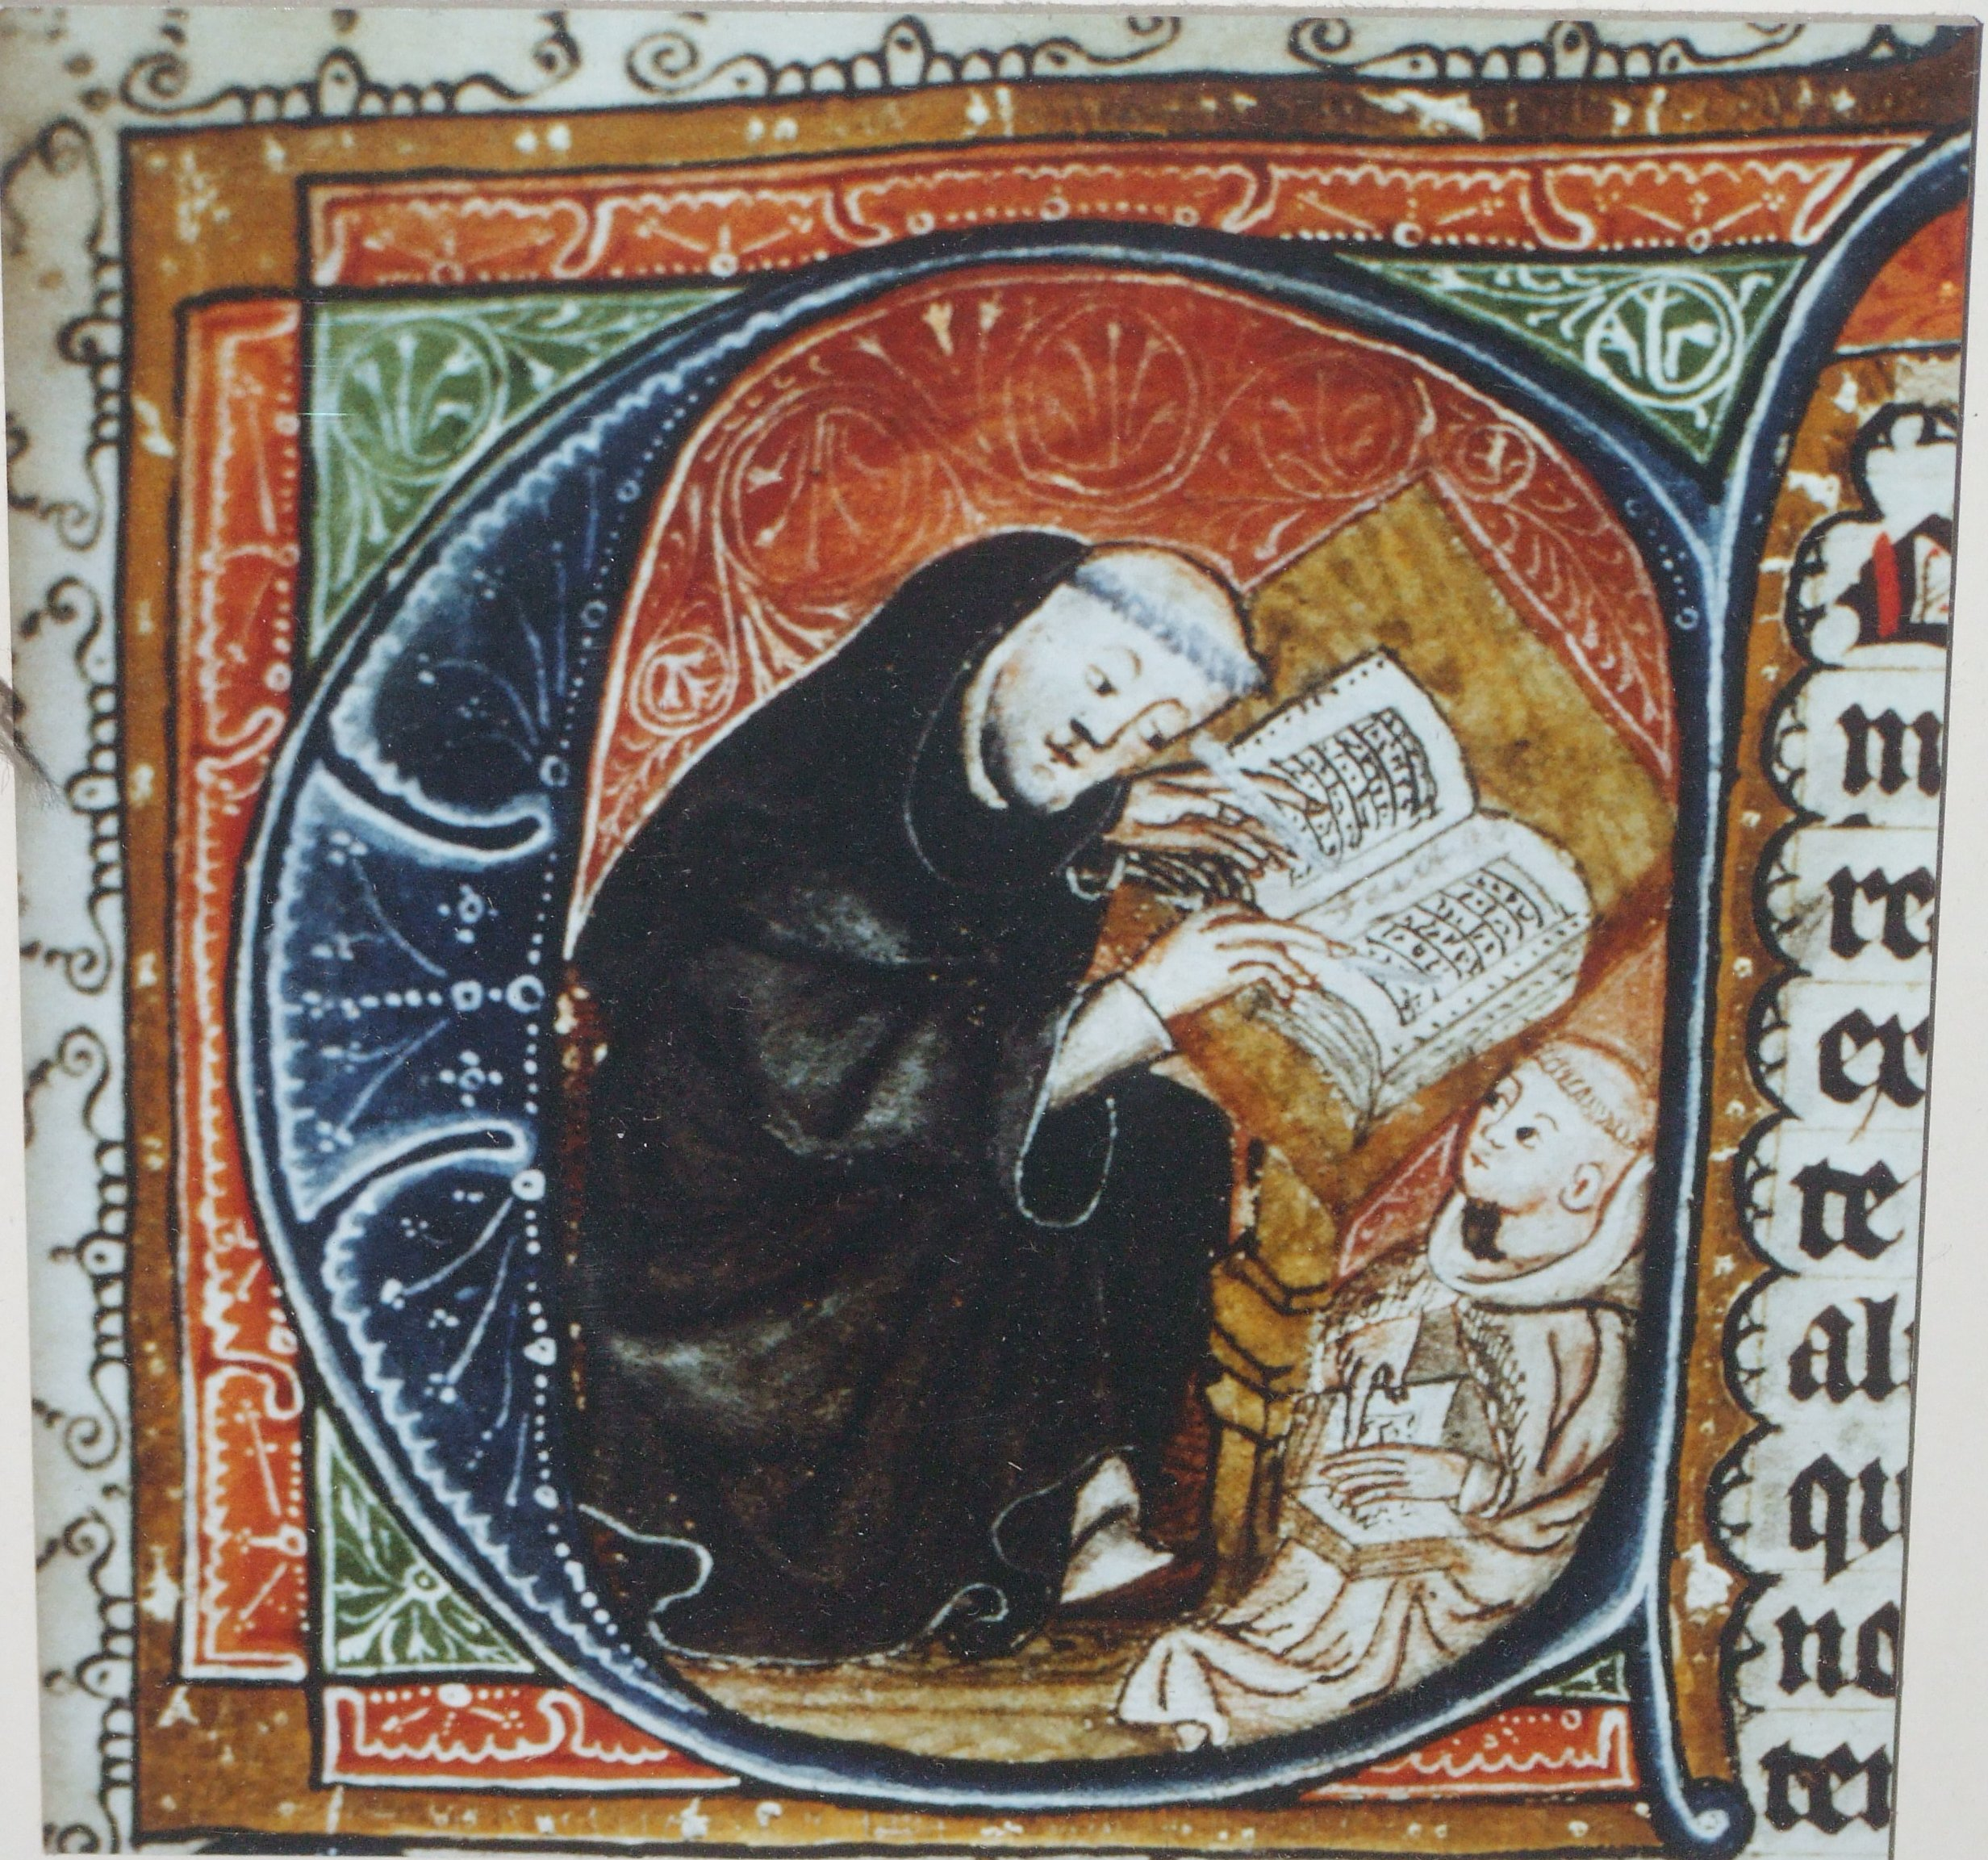
\includegraphics[width=20mm]{Caesarius_von_Heisterbach_als_Novizenmeister}
 \caption{Caesarius v. Heisterbach}
\end{marginfigure}
(inkl. Bildunterschrift) und Tabellen auf den Rand zu platzieren:

\begin{lfgwcode}{}
 \begin{marginfigure}
 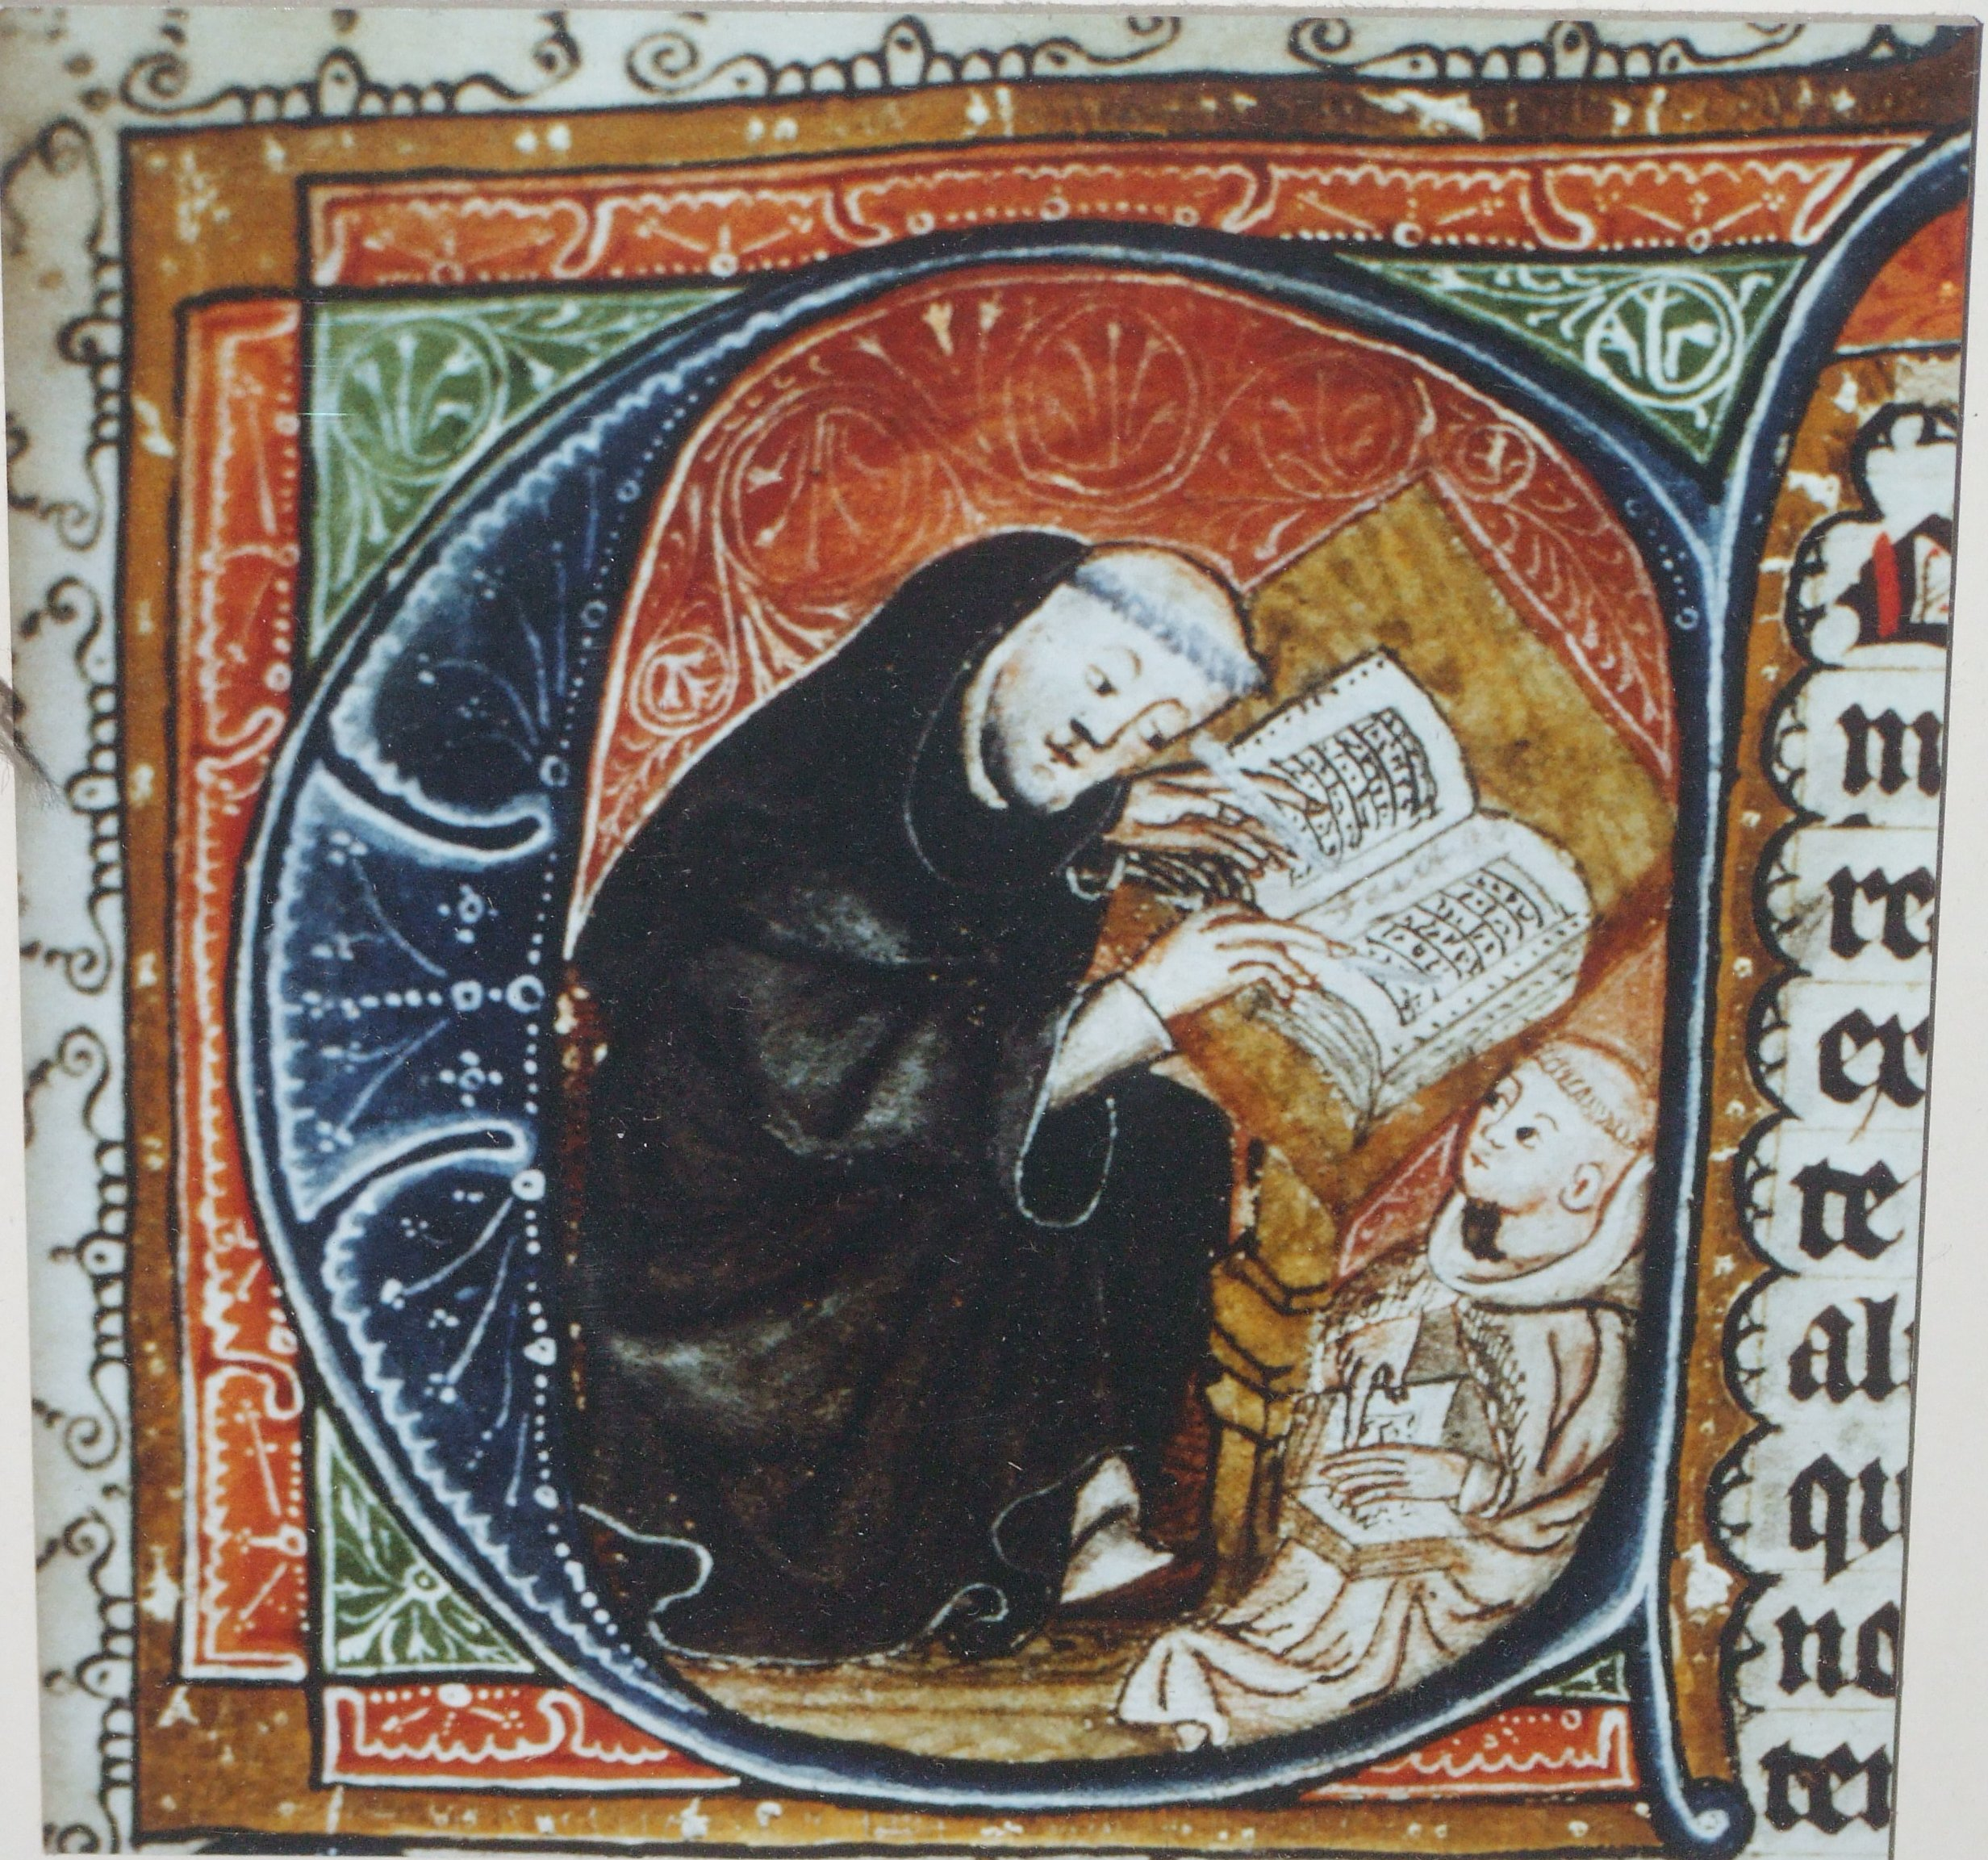
\includegraphics[width=20mm]{Caesarius_von_Heisterbach_als_Novizenmeister}
 \caption{Caesarius v. Heisterbach}
\end{marginfigure}
\end{lfgwcode}


Eine weitere Option ist, die Beschriftung einer Gleitumgebung (Bild, Tabelle) auf den Rand zu
setzen, während die Gleitumgebung selbst die gesamte Breite des Textfeldes einnimmt.

Auch Bilder und Tabellen, die sich über die ganze Seitenbreite, d.\,h. den eigentlichen Satzspiegel
\emph{und} die Marginalspalte erstrecken, werden unterstützt.

Nähere Informationen enthält die Paketdokumentation.


\section{Texte mehrspaltig setzen}

Es gibt in \LaTeX{} zwei verschiedene Wege, zweispaltigen Satz zu erreichen:
Bereits der \LaTeX{}-Kern bietet die Möglichkeit, Texte zweispaltig zu setzen;
daneben gibt es das Paket \paket{multicol}, dass mehrspaltige Einschübe in einem ansonsten
einspaltigen Dokument ermöglicht.

Beide Verfahren haben ihre Berechtigung, denn es ergeben sich jeweils verschiedene
Vor- und Nachteile bzw. Einschränkungen:

\minisec{Das ganze Dokument zweispaltig setzen}

Wird als Dokumentklassen-Option \lstinline/twocolumn/ angegeben, wird das Dokument 
zweispaltig gesetzt. 
Der Titel mit Datum, Autorangabe, Abstract etc. werden als einspaltiger Kopf über beide 
Spalten gesetzt.


\minisec{Zweispaltige Einschübe in einem einspaltigen Dokument I: \LaTeX}

Daneben bietet \LaTeX{} die Möglichkeit, in einem Dokument eine zweispaltige Passage
zu integrieren. Die Passage wird mit dem Befehl \lstinline/\twocolumn[xxx] /
eingeleitet. Die angegebene Überschrift wird einspaltig über beide Spalten gesetzt.
Außer einer echten Überschrift (z.\,B. \lstinline/\section{}/) sind hier auch
längere Einleitungstexte etc. möglich.

Mit dem Befehl \lstinline/\onecolumn/ wird wieder auf einspaltigen Satz zurückgestellt.

Beide Kommandos beginnen jeweils eine neue Seite, was ihre praktische
Benutzbarkeit meines Erachtens nach stark einschränkt.


\minisec{Mehrspaltige Einschübe in einem einspaltigen Dokument II: \paket{multicol}}

\begin{multicols}{2}
 Die umfassendste Funktionalität bietet das Paket \paket{multicol} von Frank Mittelbach.
 Mit ihm lassen sich beliebige Textpassagen in mehreren Spalten in ein ansonsten
 einspaltiges Dokument einfügen.
 
 Der Beginn einer mehrspaltigen Passage wird durch \lstinline/\begin{multicols}{Zahl}/ 
 eingeleitet; die entsprechende Anweisung \lstinline/\end{multicols}/ schaltet wieder
 auf einspaltigen Satz um. \lstinline/Zahl/ steht dabei für die Anzahl der gewünschten 
 Spalten.                                            
\end{multicols}

\setlength{\columnseprule}{0.4pt}
\begin{multicols}{3}
 Dabei liegt es in der Verantwortung des Nutzers, nicht zu viele Spalten zu verlangen,
 da sonst die einzelnen Spalten zu schmal werden und sich Aussehen und Lesbarkeit erheblich
 verschlechtern.
 
 Faustregel: Der Wortabstand soll niemals größer sein als der Zeilenabstand.
 Evtl. kann es helfen, mehrspaltige Abschnitte im Flattersatz zu setzen.
 In typografischer Hinsicht ist dies ein sehr schlechter Absatz \dots
 
 Um dem Leser zu ermöglichen, die Spalten besser wahrzunehmen kann der Längenwert 
 \lstinline/columnseprule/ auf einen Wert größer 0 gestellt werden;
 in diesem Beispiel liegt er bei 0.4pt: \lstinline/\setlength{\columnseprule}{0.4pt}/.
 
 Daneben bietet das Paket weitere Einstellmöglichkeiten, wie. z.\,B. den Spaltenabstand
 oder die Farbe der Trennlinie.
\end{multicols}



\section{Das Konzept der \enquote{Gleitumgebung}}
\dictum[Heraklit?]{Alles fließt.}

\minisec{Gleitumgebungen beschriften: Das Paket \paket{caption}}

\section{Grafiken einbinden}
\label{grafik-einbinden}
\index{Grafik} 
\index{Bilder}
\index{Abbildungen}

Voraussetzung: Paket \paket{graphicx} in Dokumentpräambel einbinden:
\lstinline/\usepackage{graphicx}/.

Dann fügt der Befehl \lstinline/\includegraphics[Optionen]{Name}/ an der jeweiligen Stelle
die angegebene Grafik (als eigenen Absatz) ein.
Als Option sollte z.\,B. die gewünschte Abbildungsgröße eingestellt werden.
Wieder sind sowohl absolute Angaben möglich als auch Bezugnahmen z.\,B. auf 
\lstinline/\textwidth/.

Meist möchte man die Abbildung jedoch in eine Gleitumgebung einfügen, so dass das Satzprogramm
flexibler die Positionierung entscheiden kann (s. vorheriger Abschnitt).
Dazu dient die Umgebung \lstinline/figure/.
Dann ist auch die Angabe einer Bildunterschrift mit dem Paket \paket{caption} möglich.

Ggf. empfiehlt sich auch noch das Einbetten in eine \lstinline/center/-Umgebung,
um das Bild auf die Mitte des Satzspiegels zu zentrieren.

Alles zusammen sieht dann so aus:

\begin{lstlisting}
\begin{figure}
 \begin{center}
  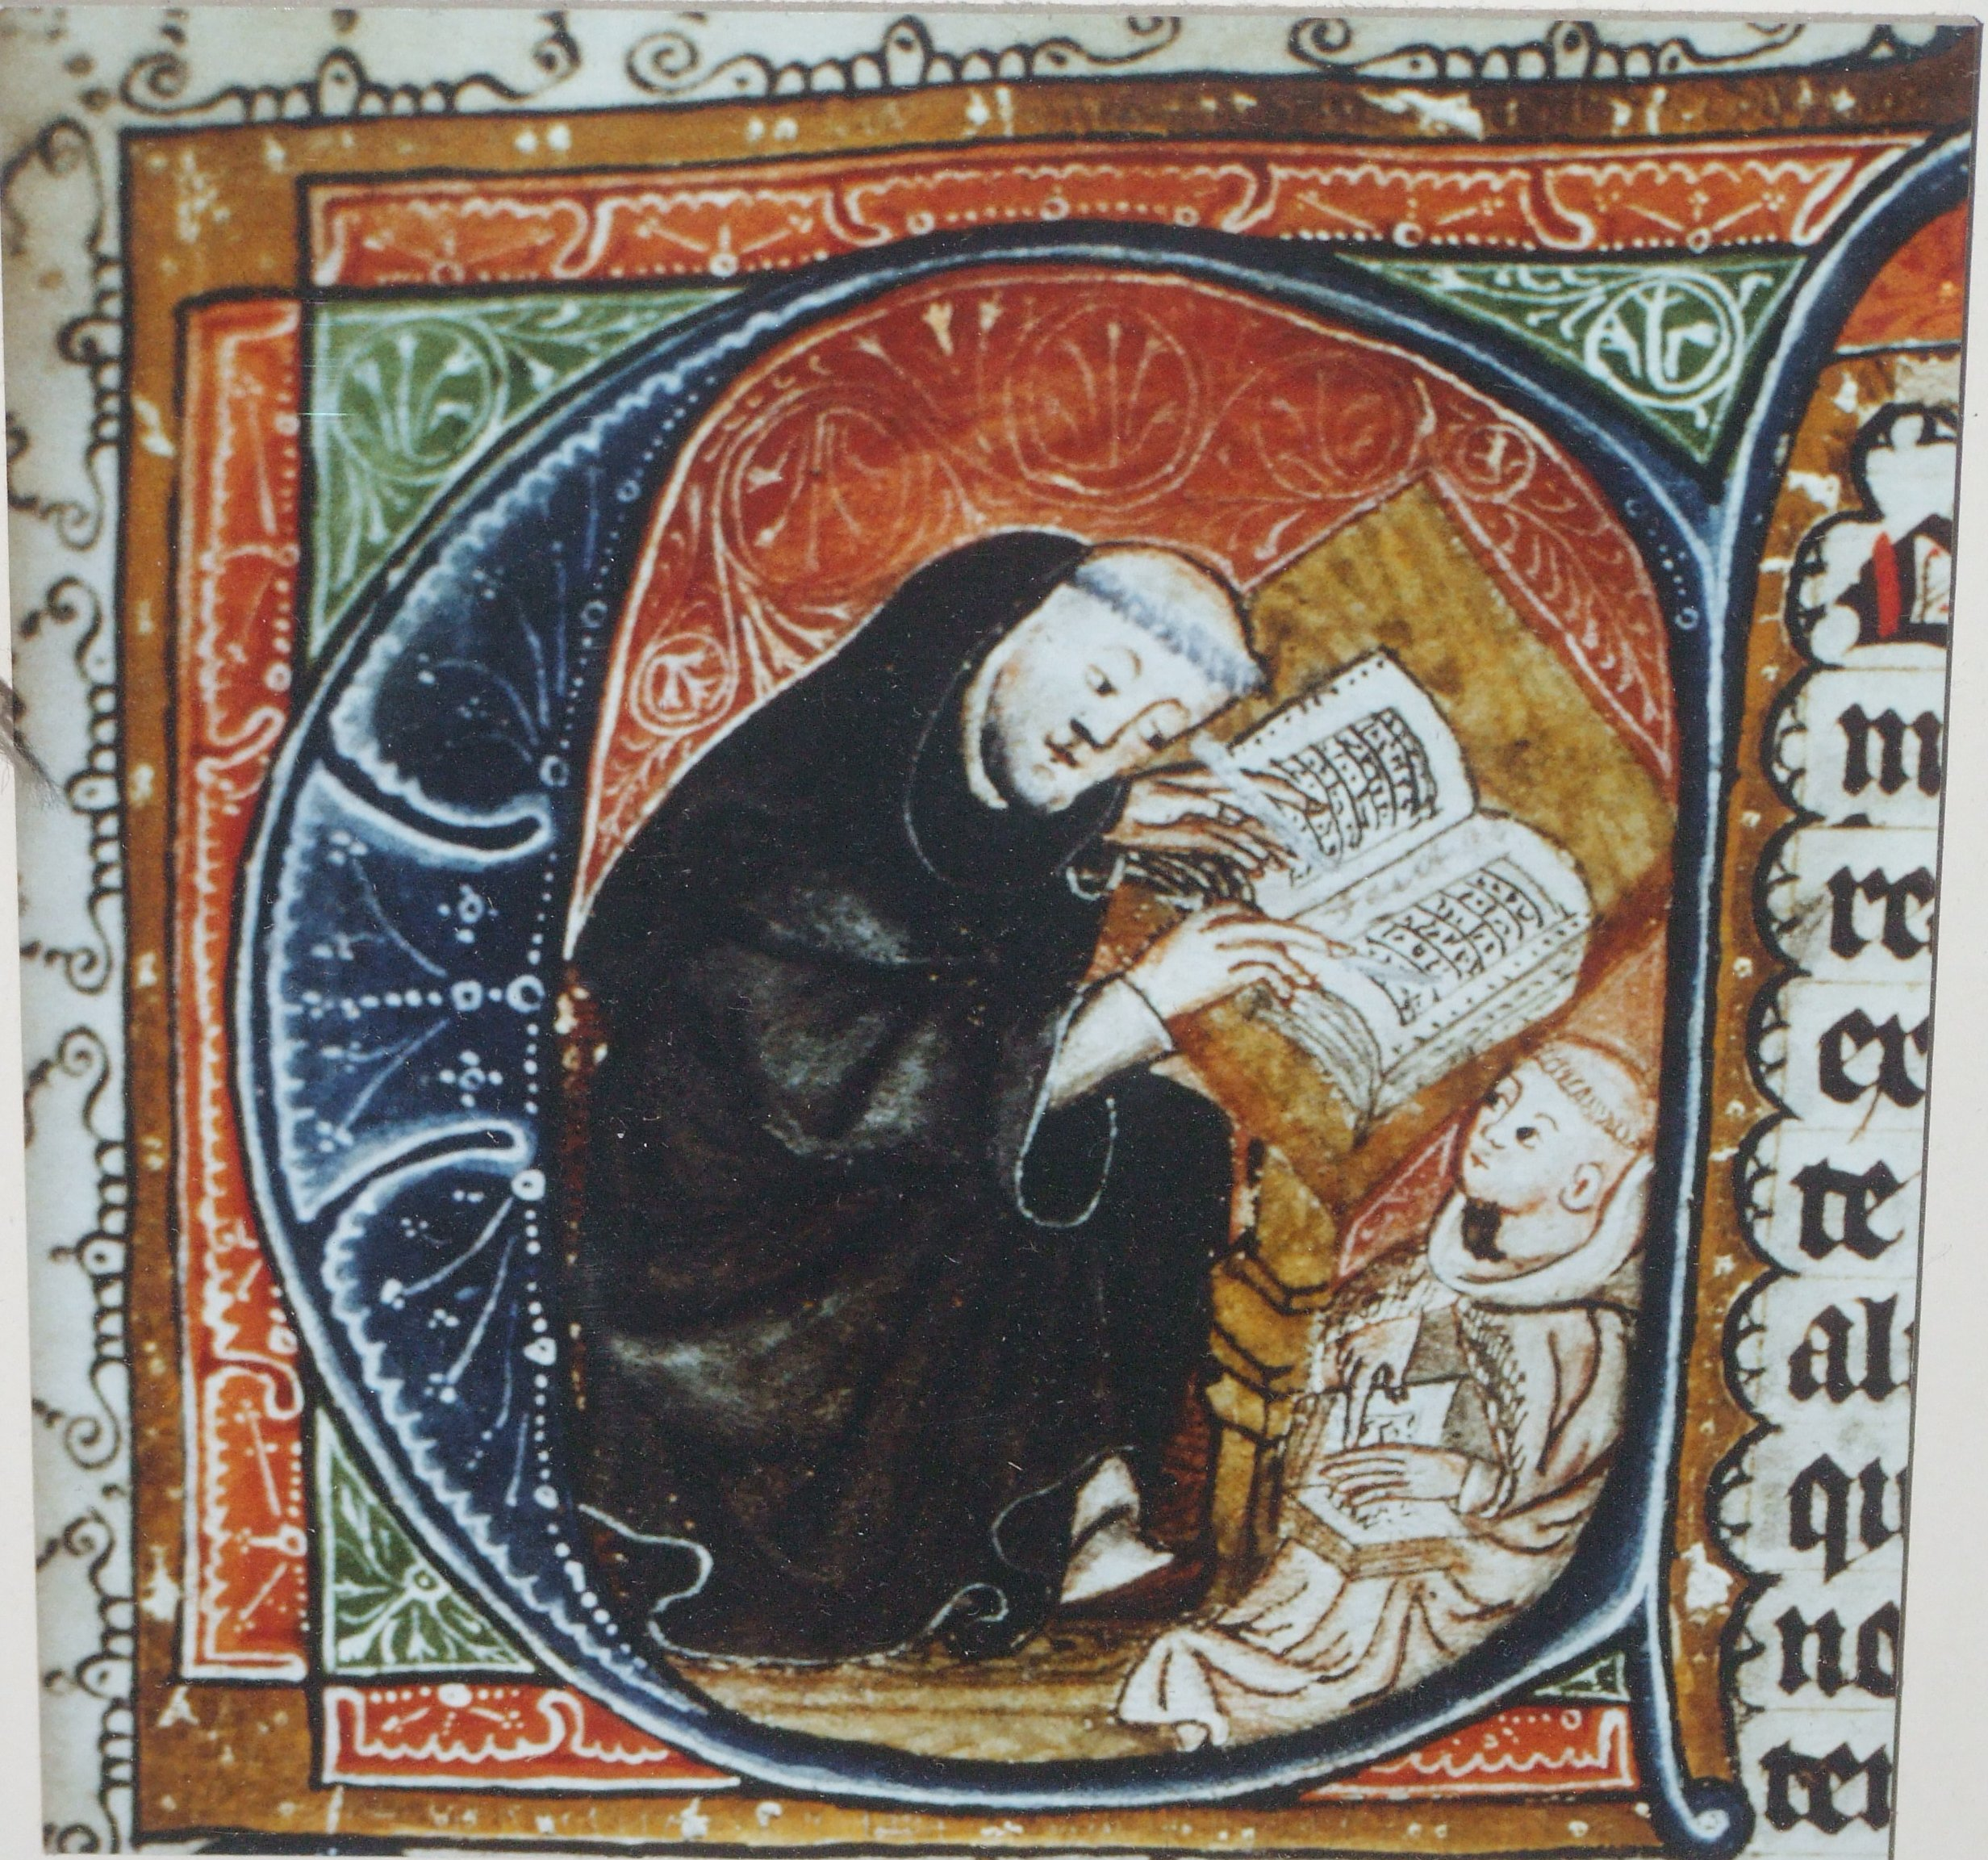
\includegraphics[width=.5\textwidth]{Caesarius_von_Heisterbach_als_Novizenmeister}
  \caption{Caesarius von Heisterbach als Novizenmeister}
 \end{center}
\end{figure} 
\end{lstlisting}


\begin{figure}[!htb]
\centering
  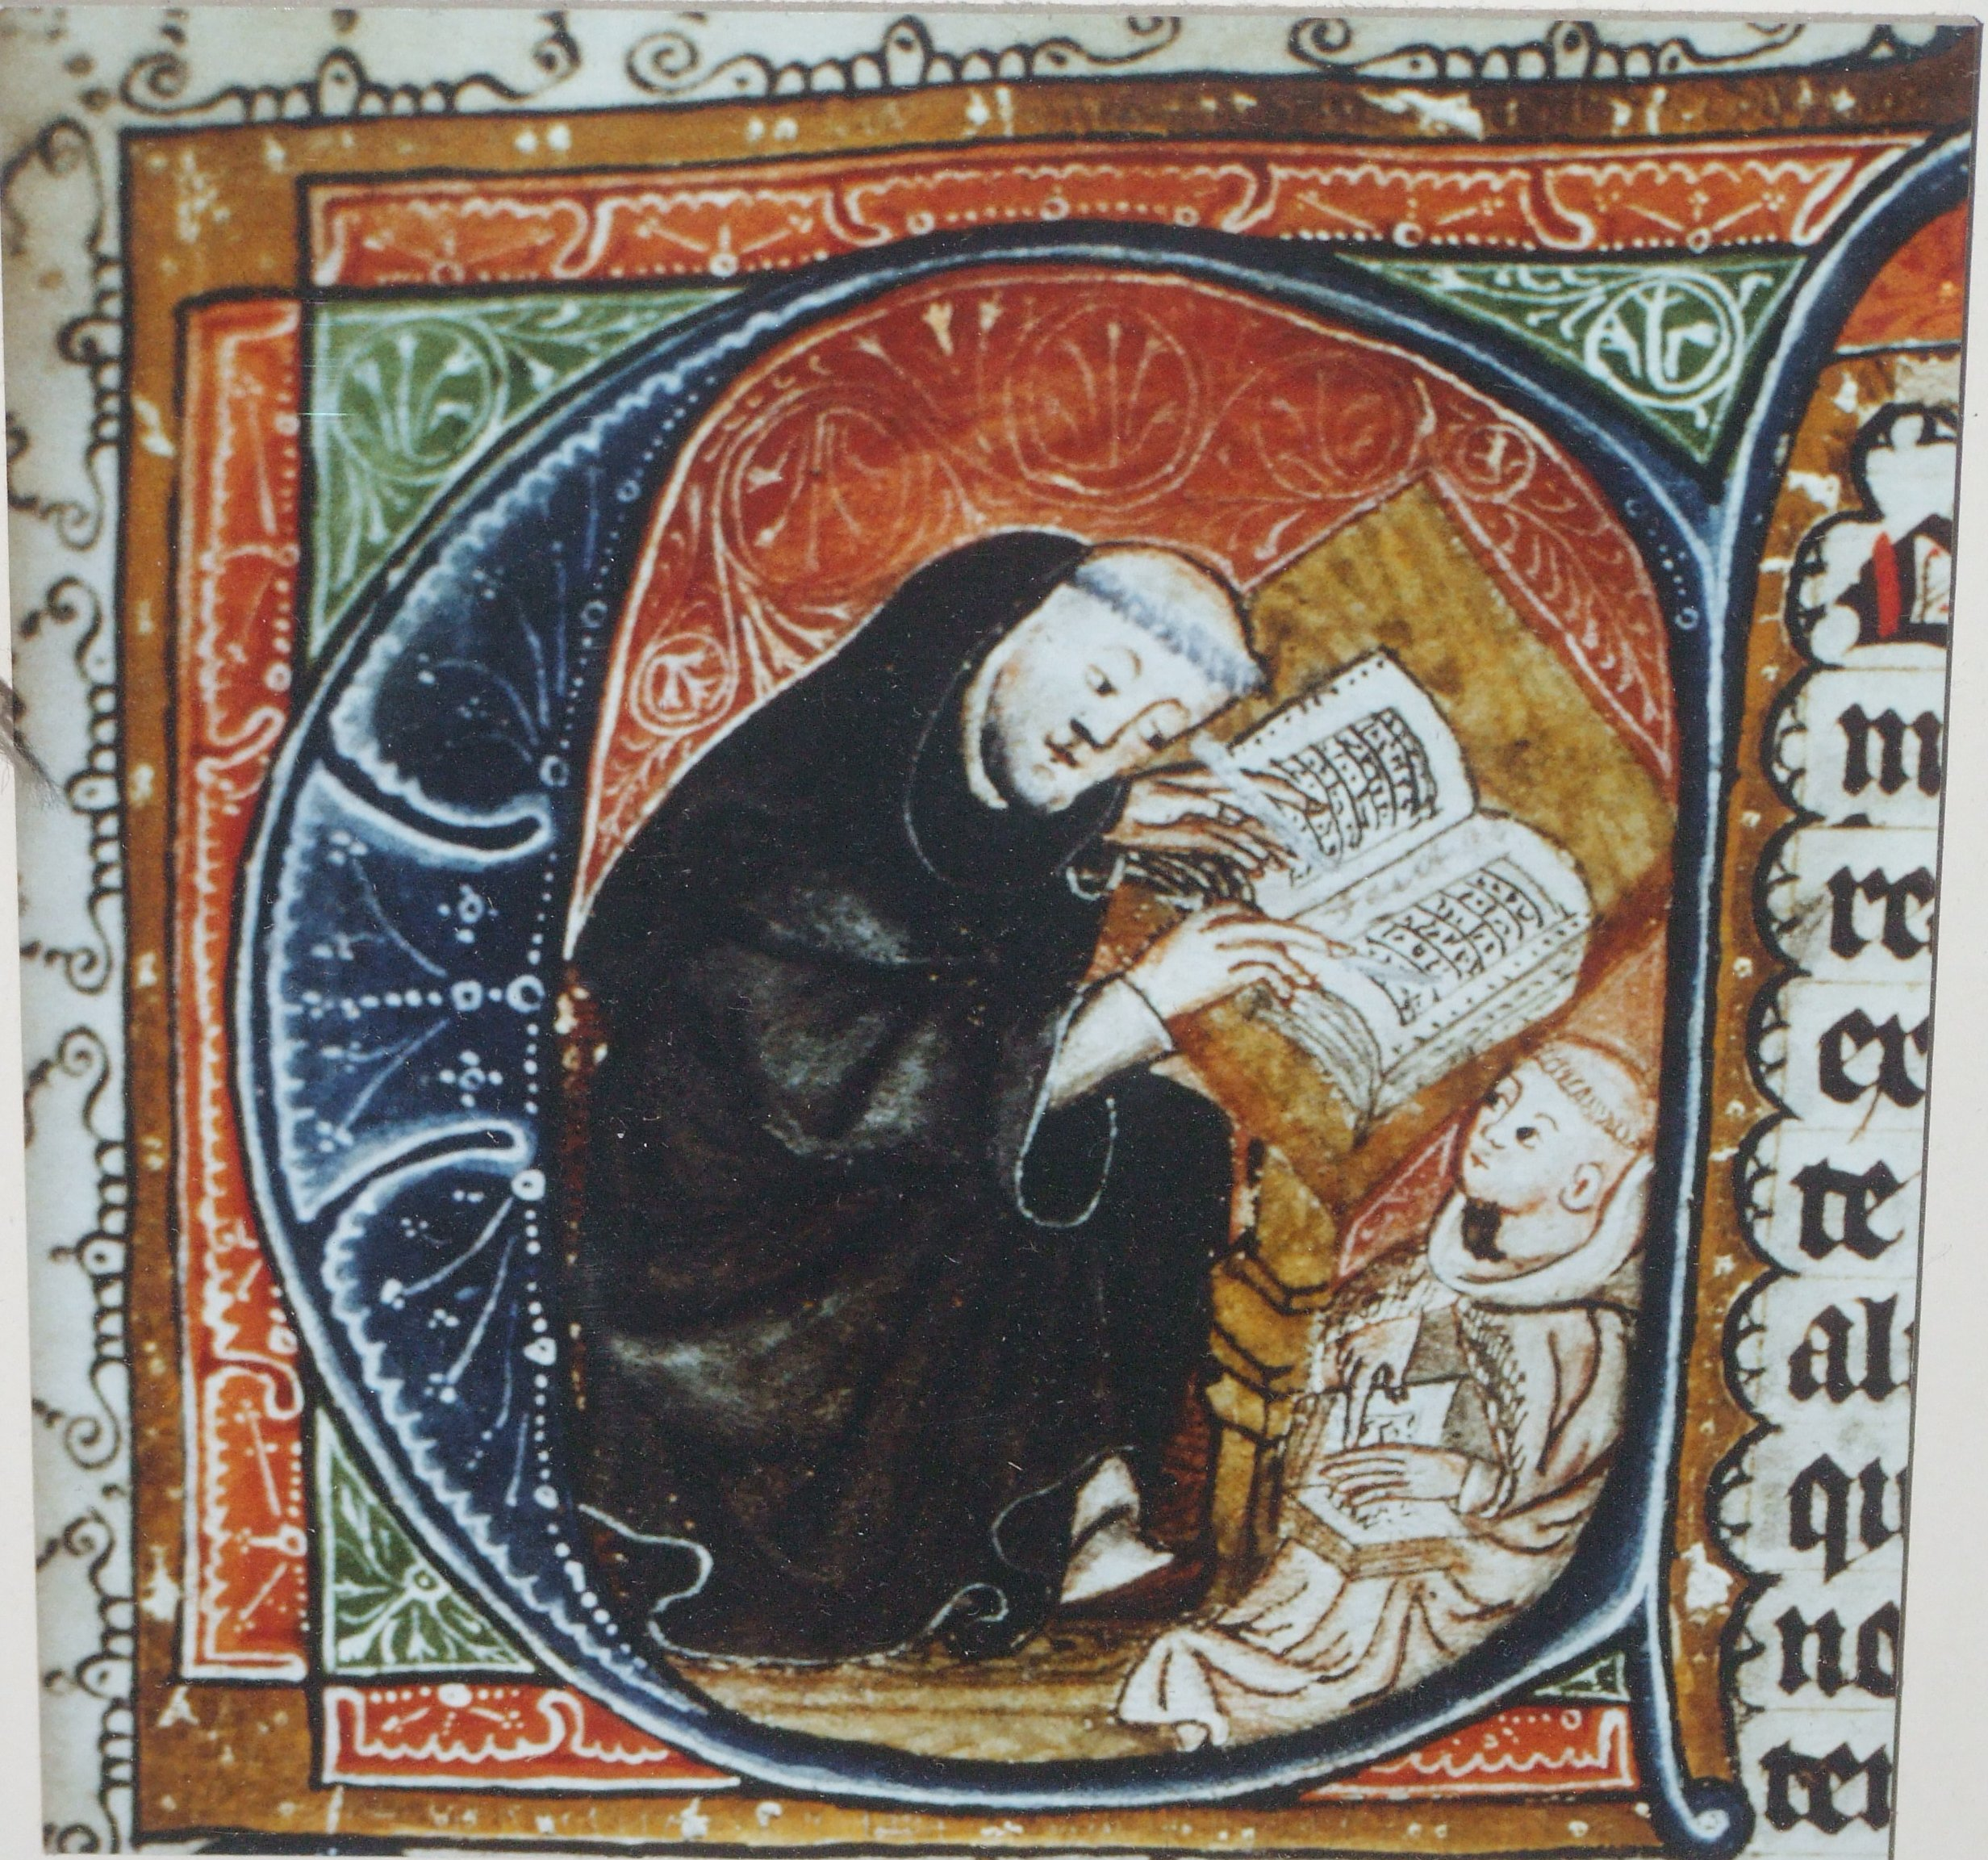
\includegraphics[width=.7\textwidth]{Caesarius_von_Heisterbach_als_Novizenmeister}
  \caption{Caesarius von Heisterbach als Novizenmeister}
\end{figure}

\section{Unter-Abbildungen mit \protect\paket{subcaption}}


\section{Tabellen erstellen}

Komplexes Thema, Spezialliteratur gerechtfertigt.\footcite{voss:tabellen}


\paket{tabularx}

\paket{longtable}

\minisec{Tabellen drehen}
\index{Drehen von Texten}

\paket{rotatebox}


\section{Umgang mit Bibelstellen}
\index{Bibelstellen}

Vor allem im Rahmen größerer Projekte empfiehlt es sich dringend, Bibelstellenangaben nicht einfach
\enquote{frei Hand} in den Text zu schreiben, sondern diese in einer eindeutigen Form 
-- mit Hilfe eines \LaTeX{}-Befehls, der auszuzeichnen. 
Dafür gibt es zwei Gründe:

\begin{itemize}
    \item Wenn man die Bibelstellenangaben auszeichnet, kann man in seinem Editor rasch alle
    Stellenangaben aufsuchen, etwa um sie nachzuschlagen, auf Vollständigkeit zu überprüfen etc.
    \item Die eindeutige Auszeichnung ist Voraussetzung für eine automatische Erfassung in einem
    Index.
    \item Während der langen Rezeptionsgeschichte der Bibel haben sich verschiedene Standards der 
    Bezeichnung der einzelnen biblischen Bücher herausgebildet. Stützt man seine Stellenangaben
    auf eine eindeutig definierte maschinenlesbare Codierung, kann man den Computer automatisch 
    dafür sorgen lassen, dass alle Bibelstellenangaben einer bestimmten Wiedergabekonvention folgen.
    Also, dass z.\,B. das erste Buch der Bibel einheitlich entweder als \enquote{Genesis} oder als \enquote{1. Buch Mose}
    referenziert wird.
\end{itemize}

Im Folgenden geht es darum, für die Zitierweise von Bibelstellen eine eindeutige Codierung zu verwenden, 
die es einerseits ermöglicht, die auftretenden Bibelstellenangaben eindeutig und automatisch 
verarbeitbar zu erfassen. 
Andererseits soll die Erfassung möglichst komfortabel sein, das heißt möglichst wenige 
kryptische Steuerzeichen in den Text bringen und außerdem in gewissen Grenzen tolerant gegenüber 
menschlicher Uneinheitlichkeit und Neigung zu Fehlern sein.

Zweck dieses Codierungsaufwandes ist die einheitliche Formatierung der Bibelstellenangaben
entsprechend etablierter Leitlinien sowie die automatische Erstellung eines Bibelstellenregisters.

Zu diesem Zweck existieren auf \url{https://ctan.org} mehrere Pakete, die den Umgang 
auch mit großen Mengen an Bibelstellenangaben sehr komfortabel machen:

\begin{itemize}
    \item \paket{bibleref} 
    \item \paket{bibleref-german} 
    \item \paket{bibleref-parse} 
\end{itemize}

\minisec{Das Paket \paket{bibleref}}

Das Paket \paket{bibleref} von Nicola Talbot bietet die genannten Vorzüge, richtet sich aber primär
an die Bedürfnisse englischsprachiger Nutzer. 
Dennoch lohnt sich ein Blick auf das Paket, weil es die konzeptionelle Grundlage für
\paket{bibleref-german} bildet, dessen Funktionsweise man verstanden haben sollte.

\paket{bibleref} stellt hauptsächlich zwei Makros bereit, die zuallererst wichtig sind:

\begin{itemize}
    \item \lstinline/\bibleref { Buch } ( Verse )/ dient zur Angabe einer Bibelstelle. 
    Für Buch ist ein definiertes Kürzel einzugeben, dass in der Ausgabe ggf. durch eine vollständigere
    Schreibweise einheitlich ersetzt wird. (Das lässt sich einstellen; verschiedene Stile sind vordefiniert.)
    \item \lstinline/\ibibleref { Buch } ( Verse )/ dito, zugleich wird im Bibelstellenregister (s.u.)
    ein Eintrag vorgenommen.
\end{itemize}

Mit diesen beiden Befehlen lassen sich Bibelstelleneingaben eindeutig bezeichnen und deshalb
mit Programmhilfe einheitlich formatiert ausgeben und im Register erschließen. 
Voraussetzung ist natürlich das Einbinden des Paketes in der Präambel:
\lstinline/\usepackage{bibleref}/
Ein Beispiel: 

\begin{lfgwcode}{}
Es gibt vier Evangelien: 
\ibibleverse{Mt}, 
\ibibleverse{Mk}, 
\ibibleverse{Lk} und \ibibleverse{John}.

Diese Stelle kommt nicht ins Register: \bibleverse{Rev}(13:15-17), 
während diese dort schon erscheint: \ibibleverse{John}(3:17).
Die Bergpredigt steht übrigens in \ibibleverse{Mt}(5-7:).
\end{lfgwcode}

Die Bearbeitung mit \LaTeX\ führt dazu, dass die Bibelstellen einheitlich formatiert ausgegeben werden:

\begin{quotation}
    Es gibt vier Evangelien: Matthew, Mark, Luke und John.
    Diese Stelle kommt nicht ins Register: Revelation 13:15–17, während diese dort schon
    erscheint: John 3:17. Die Bergpredigt steht übrigens in Matthew 5–7.
\end{quotation}

Doch das Paket hat noch mehr zu bieten:
\paket{bibleref} erlaubt, durch optionale Angabe eines Zitierstiles,%
\footnote{Paketoption \lstinline|biblerefstyle|.}
die Bibelstellen auf verschiedene
Weise auflösen zu lassen:
\lstinline/\usepackage[biblrefstyle=...]{bibleref}/

Zur Wahl stehen angloamerikanische und international verbreitete Zitierstile:

\begin{labeling}{anglosaxon}
    \item[default] 2 Corinthians 12:1-5
    \item[jerusalem] 2 Co 12:1-5
    \item[anglosaxon] II Cor. XII.1-5
    \item[JEH] 2 Cor. xii. 1-5
    \item[NTG] 2 Cor xii, 1-5
    \item[MLA] 2 Cor. xii.1-5
    \item[chicago] 2 Cor. xii: 1-5
    \item[text] Second Epistle to the Corinthians, chapter twelve verse one to five
\end{labeling}

Betrachtet man die entstandene Ausgabe unseres Beispieltextes, so fallen
dem deutschen Leser (mindestens) vier Wünsche ein, die der unmittelbaren Verwendung von
\paket{bibleref} in deutschsprachigen Texten im Wege stehen: 

\begin{itemize}
    \item Einzelne Kürzel sind im deutschen Sprachraum unhandlich: \enquote{John} statt \enquote{Jo}.
    (Übrigens: Verwendet man die Abkürzung \enquote{Jo}, wird diese zu \enquote{Joel} expandiert.)
    \item Die in der Ausgabe erzeugten Bezeichnungen der biblischen Bücher sind englisch bzw. 
    -- je nach eingestelltem Zitierstil -- lateinisch.
    \item Die Zeichensetzung der ausgegebenen Stellenangaben ist für deutsche Gewohnheiten ungewohnt: 
    Wir erwarten statt Angaben wie \enquote{Gen 1:1} eher das Format \enquote{Gen 1,1}: 
    Buch -- Kapitel -- Komma -- Vers.
    \item Die Codierung der Versangaben im Quelltext ist etwas unhandlich.
\end{itemize}

Alle vier Einschränkungen lassen sich umgehen; 
für die ersten drei Punkte hilft \paket{bibleref-german}, 
für die letzte Einschränkung wurde \paket{bibleref-parse} entwickelt.
Es ist besonders praktisch, dass sich beide Pakete kombinieren lassen.


\minisec{Das Paket \paket{bibleref-german}}

Das Paket \paket{bibleref-german} wurde von Dr. Dominik Waßenhoven entwickelt und bietet die Leistungen von \paket{bibleref} 
angepasst an die Bedürfnisse deutscher Nutzer.

Es stellt im deutschsprachigen Raum das Standardwerkzeug zum Umgang mit Bibelreferenzen dar,
deshalb soll seine Funktionalität etwas genauer demonstriert werden.

Mit Hilfe von \paket{bibleref} erstellte Dokumente sind unverändert lauffähig, wenn man nur
den Paketaufruf austauscht. (Übrigens stehen auch die englischsprachigen Ausgabeformate von
\paket{bibleref} unter \paket{bibleref-german} zur Verfügung.)

Das Ergebnis desselben Eingabetextes wie oben entspricht weit mehr deutschen Erwartungen, wenn man
nur den Paketaufruf in der Präambel ersetzt 
(\lstinline/\usepackage{bibleref-german}/): XXXX

\begin{quotation}
    Es gibt vier Evangelien: Matthäus, Markus, Lukas und Johannes.
    Diese Stelle kommt nicht ins Register: Offenbarung 13,15–17, während diese dort schon
    erscheint: Johannes 3,17. Die Bergpredigt steht übrigens in Matthäus 5–7.
\end{quotation}

%\begin{figure}
%\includegraphics[scale=.5]{listing_bibleref-german}
%\caption{Das Ergebnis von Listing 2.}
%\end{figure}

Das Ersetzen von \paket{bibleref} durch \paket{bibleref-german} hat 
drei Dinge zur Folge:

\begin{itemize}
    \item Das Paket \enquote{versteht} als Eingabe sowohl die im deutschsprachigen Raum üblichen Kürzel -- übrigens
    auch die englischen -- als auch die ausgeschriebenen Buchnamen. Man braucht keine Namenskonventionen
    zu \enquote{lernen}, meistens versteht biblref-german, welches Buch man meint. 
    Teilweise sind mehrere Bezeichnungen für das gleiche Buch definiert -- z.B. sind Numeri, Num, 4Mos und
    IVMos gleichbedeutend.
    (Selbstverständlich enthält die Paketdokumentation eine vollständige Auflistung der Buchbezeichnungen.)%
    \footnote{Achtung! Die Eingabecodierung \enquote{Jo} wird zum Buch Joel aufgelöst; das Johannes-Evangelium
        ist als \enquote{Joh} einzugeben, was dann bei Verwendung des Vulgata-Stils zu Io interpoliert wird. 
        So kompliziert kann die Welt sein\ldots }
    \item In der Ausgabe erscheinen deutsche Buchtitel.
    \item Die Zeichensetzung entspricht deutschen Gewohnheiten.
\end{itemize}

Über die Konfigurationsmöglichkeiten des englischsprachigen \paket{bibleref} lässt sich das Ausgabeformat der Bibelstellenangaben bei \paket{bibleref-german} in
zweierlei Weise modifizieren:

\begin{itemize}
    \item Zitierstil:
    Durch die Angabe als Paketoption oder alternativ mit \cs{biblerefstyle\marg{Stil}} lässt sich die Ausgabekonvention verändern.
    Mögliche Werte sind die im deutschsprachigen Raum meist verwendeten Standards: 
    \begin{itemize}
        \item \lstinline/Einheitsübersetzung/ (der voreingestellte Standardwert),
        \item \lstinline/Lutherbibel/ (in der Form von 1984),
        \item \lstinline/LThK/ (die Konventionen des Lexikons für Theologie und Kirche),
        \item \lstinline/RGG/ (Religion in Geschichte und Gegenwart),
        \item \lstinline/TRE/ (Theologische Realenzyklopädie) und 
        \item \lstinline/Vulgata/ (die lateinischen Bezeichnungen der Vulgata).
    \end{itemize}
    
    \item Format:
    Für jeden dieser Zitierstile definiert \paket{bibleref-german} noch vier Formate, die die Wiedergabe der
    Stellenangaben definieren und durch den Befehl \lstinline/\biblerefformat{<Format>}/ eingestellt
    werden können:
    
    \begin{itemize}
        \item kurz -- Offb 13,17
        \item lang -- Offenbarung 13,17
        \item Terminus -- Die Offenbarung des Johannes 13,17
        \item Zahlwort -- Die Offenbarung des Johannes, Kapitel dreizehn, Vers siebzehn
    \end{itemize}
    
\end{itemize}

Mit beiden Angaben lässt sich die Ausgabe der Belege sehr differenziert an die eigenen Bedürfnisse 
anpassen:

%\lstinputlisting[caption=Beispiel 3: Die selbe Stelle in verschiedenen Formaten und Stilen]
%    {listing_bibleref-german_stile}

\begin{lstlisting}
\documentclass{scrartcl} 
\usepackage[utf8]{inputenc}
\usepackage[T1]{fontenc}
\usepackage[ngerman]{babel}

\usepackage{bibleref-german}

\begin{document}
\bibleverse{Jo}(1:1)

\bibleverse{Joh}(3:17) 

\biblerefstyle{Vulgata}
\bibleverse{Offb}(1:1)

\biblerefformat{lang}
\bibleverse{Offb}(1:1)

\biblerefstyle{LThK}
\bibleverse{Joh}(3:17) 

\biblerefformat{Terminus} 
\bibleverse{Joh}(3:17) 

\biblerefformat{Zahlwort}
\bibleverse{Joh}(3:17)

\biblerefstyle{Vulgata} 
\biblerefformat{kurz}
\bibleverse{Joh}(1:1)
\end{document}
\end{lstlisting}

Es ergibt sich eine erstaunliche Variationsbreite an Zitiermöglichkeiten:

\begin{quotation}
    Joël 1,1 
    
    Johannes 3,17
    
    Apc 1,1
    
    Apocalypsis 1,1
    
    Johannes 3,17
    
    Das Evangelium nach Johannes 3,17
    
    Das Evangelium nach Johannes, Kapitel drei, Vers siebzehn
    
    Io 1,1
\end{quotation}


Die Formate Terminus und Zahlwort sind im Deutschen wegen der notwendigen Flexion der bestimmten Artikel 
problematischer als die englischsprachigen \texttt{text}-Variante des Paketes \paket{bibleref}. 
Ihre Benutzung ist wahrscheinlich eher die Ausnahme.
Anzumerken ist, dass der Stil Zahlwort ausgaben wie ``Kapitel one'' ergibt, wenn nicht mit babel
die Sprache auf german (oder ngerman) eingestellt wurde. Das Babel-Paket muss vor bibleref-german
eingebunden werden.

Selbstverständlich muss der verantwortungsbewusste Textautor selbst entscheiden, in welchem Maße
das Vermischen verschiedener Formate und insbesondere Stile innerhalb eines Dokumentes sinnvoll ist.

Mit \paket{bibleref-german} lassen sich die deutschsprachigen Gepflogenheiten bei der Formatierung von
Bibelstellenangaben sehr präzise abbilden. Wenn jetzt noch das Eingabeformat (hinsichtlich Kapitel- und
Versangabe) etwas handlicher wäre \dots


\subsection{Das Paket \paket{bibleref-parse}}

Genau dies ist das Ziel des Paketes \paket{bibleref-parse} von Sebastian Kuhnert:
\enquote{The bibleref-parse package parses Bible passages that are given in a human readable format.}
\footnote{Sebastian Kuhnert, The bibleref-parse Package, S. 1}
Die beiden wichtigsten Befehle, die von dem Paket definiert werden, lauten analog zu
\paket{bibleref} und \paket{bibleref-german}:

\begin{itemize}
    \item\lstinline/\pbibleref { Buch mit Kapitel- u. Versangabe } / (Man beachte das \textbf{p}!) 
    \footnote{Die Umbenennung der beiden Befehle ist deshalb nötig, weil innerhalb desselben 
        Dokuments sowohl Bibelstellen im Eingabeformat von \paket{bibleref} bzw. \paket{bibleref-german} als auch 
        im Format von \paket{bibleref-parse} möglich sind. Wahrscheinlich ist es empfehlenswert, bei einer größeren
        Arbeit sich auf \paket{bibleref-parse} festzulegen und eine eigene Abkürzung zu definieren, z.B. 
        \lstinline/bibel/ für normale Stellen und \lstinline/bibelx/ für Stellen, die im Index
        erfasst werden sollen.}
    definiert einen Bibelstellenverweis.
    \item\lstinline/\pibibleref { Buch mit Kapitel- u. Versangabe } / (nicht vergessen: \textbf{p}!) dito, zugleich wird im Bibelstellenregister (s.u.)
    ein Eintrag vorgenommen.
\end{itemize}

Mit ihnen ist es möglich, Bibelstellen so zu zitieren, wie es der deutschsprachige Nutzer gewohnt ist.
Dabei stellt sich der Parser sehr weitgehend auf die vielen Sonderfälle ein, die in Bibelstellen 
auftreten können. Deshalb ist die Hauptregel ganz einfach:
\enquote{The  basic message is: Just use your intuition. This is what this package was created for.}%
\footnote{ebd. S. 3.}

Diese Erklärung verspricht nicht zuviel, wie das folgende Listing zeigt:
bibleref-parse in Zusammenspiel mit biblref-german:
Bequemer geht's nicht. Nur das \enquote{p} am Beginn der Bibelstellen-Kennungen darf man nicht vergessen\ldots

%\lstinputlisting[caption=Beispiel 4: bibleref-parse in Zusammenspiel mit biblref-german:
%    Bequemer geht's nicht. Nur das ``p'' am Beginn der Bibelstellen-Kennungen darf man nicht vergessen...]
%    {listing_bibleref-german-parse}

\begin{lstlisting}
\documentclass{scrartcl} 
\usepackage[utf8]{inputenc}
\usepackage[T1]{fontenc}

\usepackage{bibleref-german} % Ausgabe: deutsche Gepflogenheiten
\usepackage{bibleref-parse}  % Eingabe: quasi künstliche Intelligenz ;-)


\begin{document}
Es gibt vier Evangelien: 
\pibibleverse{Mt}, 
\pibibleverse{Markus}, 
\pibibleverse{Luke} 
und \pibibleverse{Joh}. 
Diese Stelle kommt nicht ins Register: \pbibleverse{Offb 13,15-17}, 
während diese dort erscheint: \pibibleverse{Joh 3,17}. 
Die Bergpredigt steht übrigens in \pibibleverse{Mt 5-7}.
\end{document}
\end{lstlisting}

%\begin{figure}
%\includegraphics[scale=.5]{listing_bibleref-german-parse}
%\caption{Das Ergebnis von Listing 4.}
%\end{figure}

Nur der Vollständigkeit halber die \enquote{Auflösung} durch \LaTeX\ldots

\begin{quotation}
    Es gibt vier Evangelien: Matthäus, Markus, Lukas und Johannes. Diese Stelle kommt
    nicht ins Register: Offenbarung 13,15–17, während diese dort erscheint: Johannes 3,17.
    Die Bergpredigt steht übrigens in Matthäus 5–7.
\end{quotation}

Die Aufgabenstellung, unter Benutzung einer leicht handhabbaren, \enquote{menschenfreundlichen} Codierung
Bibelstellenangaben mit computerischer Einheitlichkeit auszugeben -- und das auch noch in verschiedenen
vordefinierten Stilen -- ist mit Hilfe von \paket{bibleref-german} und \paket{bibleref-parse} gelöst.

Damit ist zugleich die Voraussetzung für die ebenso mühelose Erstellung eines Bibelstellenindex geschaffen.

Zur Registererstellung vgl. \fullref{Bibelstellenregister}.


% Section Lyrik-Satz von Christine Römer - thm 6.3.2017

%% lfgw: 2.19 Lyrik-Satz


%% !TEX root = lfgw.tex

\RequirePackage{iftex}
\RequireLuaTeX
\RequirePackage{luatex85}

\documentclass[%
   ibycus,polutonikogreek,english,french,latin,ngerman,%global definiert!
   %%%draft=false,%
   fontsize=11pt,%
   paper=17cm:24cm,%
   DIV=13,%
   listof=totoc,%
   bibliography=totoc,%
   pagesize%
   ]{scrbook}

\KOMAoption{bibliography}{leveldown}

\usepackage{yfonts}
\usepackage{textgreek}
\usepackage{cjhebrew}[2017/03/06]
\usepackage{amsmath,amssymb} % für forrest
%%%\usepackage{textcomp}
\usepackage{unicode-math}
\usepackage{fontspec}
\defaultfontfeatures{Ligatures=TeX,Scale=MatchLowercase}
%\newfontfamily\GFSDidot{GFS Didot}
\newcommand\gkk[1]{%{\GFSDidot
#1}

\usepackage[]{babel}
%\usepackage[ngerman,noftligs]{selnolig}
%%%\setmainfont{Libertinus Serif} %reicht auch, unten evtl. besser wegen SB
\setmainfont{libertinusserif}[
   Extension = {.otf},
   UprightFont = {*-regular}, ItalicFont = {*-italic},
   BoldFont = {*-bold}, BoldItalicFont = {*-bolditalic},%
   FontFace = {sb}{\updefault}{*-semibold},%
   FontFace = {sb}{it}{*-semibolditalic}]%
\setsansfont{Libertinus Sans}
\setmonofont[Scale=MatchLowercase,FakeStretch=0.85]{DejaVu Sans}%das wird für Griechisch in Codebeispielen gebraucht
\setmathfont{Libertinus Math}
\makeatletter
\newcommand*\sustyle{\addfontfeatures{VerticalPosition=Superior}}
\DeclareTextFontCommand{\textsu}{\sustyle}
\def\@makefnmark{\hbox{\sustyle\@thefnmark}}
\makeatother
\DeclareTextCommandDefault{\textborn}{{\char"002A}}
\DeclareTextCommandDefault{\textdied}{{\char"2020}}
\usepackage[% microtype
   final,%
   tracking=smallcaps,%
   expansion=alltext,%
   protrusion=true%
   ]{microtype}%
\SetTracking{encoding=*,shape=sc}{50}%
\UseMicrotypeSet[protrusion]{basicmath} % disable protrusion for tt fonts

\usepackage[headsepline]{scrlayer-scrpage}
\clearscrheadfoot
\ihead{\headmark}
\ohead{\pagemark}
\pagestyle{scrheadings}

\usepackage[autostyle]{csquotes}
\usepackage[newcommands]{ragged2e}

\usepackage{graphicx}
\graphicspath{{bilder/}}

\usepackage{grffile}
\usepackage[a4,center,cross]{crop}

\usepackage{listings}
\lstdefinestyle{listinglfgw}{%
  inputencoding=utf8,
  extendedchars=true,
  language=[LaTeX]{TeX},
  numbers=left, 
  %stepnumber=3,
  numbersep=5pt, 
  numberfirstline=false,  
  numberstyle=\tiny\textsf,
  basicstyle=\ttfamily\footnotesize,
  keywordstyle=\bfseries,%
  texcsstyle=*\ttfamily\footnotesize\bfseries,%
  %frame=tlrb,
  breaklines=true,
  breakatwhitespace=true,
  breakindent=5pt,
  %postbreak=\mbox{$\hookrightarrow$},
  escapeinside={*@}{@*},
  %showstringspace=false, 
  captionpos=b,
  upquote=true,
  %%%classoffset=0,
  morekeywords={%
  %a
  addbibresource,addplot,Afootnote,alteSeite,autocite,autopar,answerline,alertblock,
  %b
  beginnumbering,Bfootnote,biblerefformat,biblerefmap,biblerefstyle,bonuspointpoints,bibleref,block,
  %c
  Cfootnote,chapter,chbpword,chpword,chpgword,chqword,chsword,chtword,citeauthor,cites,citetitle,columnrulewidth,Columns,columnsposition, center,
  chronology,columns,
  %d
  draw,dictum,deffootnote,deffootnote,description,
  %e
  edtext,endnumbering,enquote,enumi,example,exampleblock,
  %f
  firstlinenum,firstlinenumR,firstpageheadrule,footcite,footcites,footfullcite,fullcite,fillwithgrid,fillwithlines,fillwithdottedlines,Forest,Forest*,
  footnotemargin,fillwithlines, fillwithgrid,
  %h
  hpword,hqword,hsword,htword,hypertarget,hyperlink,hideallsubsection,
  %i
  includegraphics,includeonlyframes,ibibleref,invisible,
  %l
  Lcolwidth,ledsidenote,lemma,linenumincrement,linenumincrementR,
  %m
  msdata,mode,maketitle,multifootsep,
  %n
  newfontface,newfontfamily,node,
  %o
  only,onslide,
  %p
  Pages,parencite,parencites,part,pend,pibibleverse,pbibleverse,pointpoints,printbibheading,printbibliography,printindex,pstart,pgfimage,pgfusepath,
  pgfplothandlerlineto,pgfplotsset,pgfplotxyfile,pbibleref,pibibleref,pgf-pie,plain,
  %q
  quell,question,quote,quotaion,
  %r
  Rcolwidth,reledmac,
  %s
 selectlanguage,setlength,setmainfont,setmonofont,setmsdatalabel,setromanfont,setsansfont,smartcite,smartcites,solutiontitle,setbeamerfont,setbeamercovered,subsection,subsection*,subsubsection,subtitle,solution,solutionorgrid,
  %t
  text,textborn,textcite,textcites,textdelta,textDelta,textdied,texteuro,textgamma,textGamma,textmarried,textsubscript,thealteSeite,tableofcontents,th,TH,
  textalpha, textbeta, textgamma, textdelta, textepsilon, textzeta, texteta, texttheta, textiota, textkappa, textlambda, textmu, textnu,
  textxi, textomikron, textpi, textrho, textsigma, texttau, textupsilon, textphi, textchi,  textpsi, textomega,
  textAlpha, textBeta, textGamma, textDelta, textEpsilon, textZeta, textEta, textTheta, textIota, textKappa, textLambda, textMu, textNu,
  textXi, textOmikron, textPi, textRho, textSigma, textTau, textUpsilon, textPhi, textChi,  textPsi, textOmega, twocolumn,
  %u
  usetheme,usecolortheme,usebackgroundtemplate,useforestlibrary,usepackage,usetikzlibrary,
  %v
  vari,verse,
  %x
  Xafternumber,Xarrangement,Xlemmaseparator,Xinplaceoflemmaseparator,Xinplaceofnumber,Xnonbreakableafternumber,Xnotenumfont,Xnumberonlyfirstinline,Xnumberonlyfirstintwolines,Xsymlinenum,Xtwolines,Xtwolinesbutnotmore,Xtxtbeforenotes
  },   
  literate=
  {á}{{\'a}}1 {é}{{\'e}}1 {í}{{\'i}}1 {ó}{{\'o}}1 {ú}{{\'u}}1
  {Á}{{\'A}}1 {É}{{\'E}}1 {Í}{{\'I}}1 {Ó}{{\'O}}1 {Ú}{{\'U}}1
  {à}{{\`a}}1 {è}{{\`e}}1 {ì}{{\`i}}1 {ò}{{\`o}}1 {ù}{{\`u}}1
  {À}{{\`A}}1 {È}{{\'E}}1 {Ì}{{\`I}}1 {Ò}{{\`O}}1 {Ù}{{\`U}}1
  {ä}{{\"a}}1 {ë}{{\"e}}1 {ï}{{\"i}}1 {ö}{{\"o}}1 {ü}{{\"u}}1
  {Ä}{{\"A}}1 {Ë}{{\"E}}1 {Ï}{{\"I}}1 {Ö}{{\"O}}1 {Ü}{{\"U}}1
  {â}{{\^a}}1 {ê}{{\^e}}1 {î}{{\^i}}1 {ô}{{\^o}}1 {û}{{\^u}}1
  {Â}{{\^A}}1 {Ê}{{\^E}}1 {Î}{{\^I}}1 {Ô}{{\^O}}1 {Û}{{\^U}}1
  {œ}{{\oe}}1 {Œ}{{\OE}}1 {æ}{{\ae}}1 {Æ}{{\AE}}1 {ß}{{\ss}}1
  {ç}{{\c c}}1 {Ç}{{\c C}}1 {ø}{{\o}}1 {å}{{\r a}}1 {Å}{{\r A}}1
  {€}{{\EUR}}1 {£}{{\pounds}}1
}
\lstset{style=listinglfgw}
  
\usepackage[% tcolorbox
  skins,%
  listings,%
  breakable,%
]{tcolorbox}
\tcbset{%
lfgwstyle/.style={%
    before skip=\baselineskip,
    boxrule=0pt,
    %bottomrule=2pt,
    %toprule=2pt,
    %colframe=black,
    colback=black!5,
    coltitle=white,
    bicolor,
    sharp corners,
    colbacklower=white,
    fonttitle=\sffamily\bfseries,
    breakable,
    %label=#1,
}}


\newtcblisting[auto counter,number within=chapter]{lfgwexample}[1]{%
    lfgwstyle,
    fontupper=\small\ttfamily,
    sidebyside,
    listing and text,
    title={Beispiel \thetcbcounter},
    listing options={style=listinglfgw},
    #1,
%text and listing,
}

\newtcblisting[use counter from=lfgwexample,number within=chapter]{lfgwcode}[1]{%
    lfgwstyle,
    fontupper=\small\ttfamily,
    listing only,
    title={Beispiel \thetcbcounter},
    listing options={style=listinglfgw},
    #1,
}

\newtcblisting[use counter from=lfgwexample,number within=chapter]{lfgwprint}[1]{%
    fontupper=\small,
    lfgwstyle,
    text only,
    title={Beispiel \thetcbcounter},
    listing options={style=listinglfgw},
    #1,
}


\usepackage{showexpl}
%\lstset{explpreset={escapeinside={*@}{@*}}}

\usepackage[pagewise]{lineno}
\usepackage{sidenotes}
\usepackage{multicol}
% Für den Abschnitt über Konstituentenanylyse von C. Römer:
\usepackage[linguistics]{forest}
\forestapplylibrarydefaults{linguistics,edges}
\useforestlibrary{edges}
\makeatletter
\let\pgfmathModX=\pgfmathMod@
\usepackage{pgfplots}%
\pgfplotsset{compat=1.14}
\let\pgfmathMod@=\pgfmathModX
\makeatother
%http://tex.stackexchange.com/questions/328972/presence-of-pgfplots-package-breaks-forest-environment-%w-folder-option-en/329015

% Pakete im Bereich Kapitel 3 - Diagramme zeichnen
\usepackage{tikz}
\usepackage[all]{genealogytree}
\usepackage{chronology}
\usepackage{pgf-pie}
\usetikzlibrary{pgfplots.dateplot}
\usetikzlibrary{mindmap}

\deffootnote[1.5em]{1.5em}{1.5em}{\makebox[1.5em][l]{{\fontseries{sb}\selectfont\thefootnotemark\ }}}

\usepackage{enumitem}			% for simple list modifications
\setlist{leftmargin=*,before=\setlength{\rightmargin}{\leftmargin}}

%\usepackage{parallel}


%- Für Lyrik-Satz, Christine Römer:
\usepackage{verse}
\newcommand\He{\textbackslash\xspace}
\newcommand\Se{$\cup$\xspace} 
\newcommand*{\Zr}{\unskip\textunderscore}
\newcommand\daktylus{\textbackslash$\cup\cup$\xspace} 
\newcommand\anapaest{$\cup\cup$\textbackslash\xspace}

% ------------
\usepackage{runic}
\usepackage{hieroglf}
\usepackage[normalem]{ulem} %%% MS: Wofür? Unterstreichungen sollten vermieden werden! LCB: kann \xout
%\usepackage{letterspace} %%% MS: Wofür. Besser direkt \textls aus dem Microtypepaket
%% ------------------------------------------------------------------------
%%   This is a stand-alone version that only provides the letterspacing
%%   commands. Do not use this package together with the `microtype' package.
%%   Please refer to section 7 of the `microtype' documentation.
%% ------------------------------------------------------------------------ 
\usepackage[hyphens]{url}
\usepackage{hologo}
\usepackage{philex}
\def\fg{}
\usepackage{siunitx} %Supreme typesetting of units
%\sisetup{%
%    tight-spacing=true, %
%    %math-rm=\mathsf, 
%    %		text-rm=\sffamily,
%    detect-all, %Zahlen werden in der aktuellen Schrift angezeigt
%    detect-family,
%    exponent-to-prefix  	= true,%
%    round-mode          	= places,% 
%    round-precision     	= 2,%
%    group-minimum-digits 	= 4, % Für "Tausenderpunkt" --> 1.234 anstatt 1234
%    group-separator			={.},% für "12.345" statt "12 345"
%    %  scientific-notation = engineering, % Use multiples of 3 as exponent
%    locale					=DE, % Typeset numbers and units the German way
%    range-phrase 			={$\times$},%
%    %		zero-decimal-to-integer,%aus "2.0" wird "2"
%    range-units				=single,  % --> 2 x 2 m, - auskommentieren für 2 m x 2 m
%    %%%---------
%%    unit-color=myred,
%}

\usepackage[german]{keystroke}% Computer-Tastatur-Tasten in Anweisungs-Texte zu setzen (z.B. \Shift, \Ctrl, \Spacebar).

\usepackage{imakeidx}
\indexsetup{level = \subsection*, toclevel = subsection, noclearpage, headers = {\indexname}{\indexname}}
\makeindex[                title = {Allgemeiner Index}]
\makeindex[name = pakete,  title = {Verzeichnis der Paketnamen}]
\usepackage[% biblatex
   style=authoryear,  
%  style=historische-zeitschrift, % das am liebsten - aber der geht (bei mir?) nicht!
%  pageref=true,
	backend=biber
	]{biblatex}
\addbibresource{lfgw-bibliographie.bib}
%%%\defbibheading{bibliography}{\addchap{#1}} %%%Besser bei \addchap bleiben

\usepackage{fancyvrb}
\makeatletter
\usepackage[% reledmac
   series={A,B,C},%nur die Apparate A B C aktivieren
   noend,%keine Endotenapparate
   noeledsec%keine eledsections et al.
   %noledgroup%keine ledgroups -- das muss hier auskommentiert werden, damit die minipages funktionieren!
]{reledmac}%
\@ifpackagelater{reledmac}{2017/03/20}{%
   % Package is new enough
}{%
\PackageError{reledmac}{Es wird reledmac >= 2.18.1 benötigt.}%
}
\makeatother
\usepackage{reledpar}

\usepackage{varioref}
\usepackage{hyperxmp}
\usepackage{hyperref}
\hypersetup{					% setup the hyperref-package options
	pdftitle={LaTeX für Geisteswissenschaftler},	% 	- title (PDF meta)
	pdfsubject={Handbuch},% 	- subject (PDF meta)
	pdfauthor={varia},	% 	- author (PDF meta)
	pdfauthortitle={},
	pdfcopyright={Copyright (c) \the\year\. All rights reserved.},
	pdfhighlight=/N,
	pdfdisplaydoctitle=true,
	pdfdate={\the\year-\the\month-\the\day}
	pdflang={de},
   pdfencoding=unicode,   % Sorgt für korrekte Umlaute in den pdf-Lesezeichen - thm
	pdfcaptionwriter={varia},
	pdfkeywords={{LaTeX}, {Geisteswissenschaften}},
	pdfproducer={LuaLaTeX},
	pdflicenseurl={http://creativecommons.org/licenses/by-nc-nd/4.0/},
	plainpages=false,			% 	- 
   colorlinks   = true, %Colours links instead of ugly boxes
   urlcolor     =  blue!50!black, %Colour for external hyperlinks
   linkcolor    = blue, %Colour of internal links
   citecolor   = green!50!black, %Colour of citations
   linktoc=page,
  	pdfborder={0 0 0},			% 	-
	breaklinks=true,			% 	- allow line break inside links
 %   bookmarks=true,
	bookmarksnumbered=true,		%
	bookmarksopenlevel=2,
	bookmarksopen=true,		%
   bookmarksdepth=3,
   pdfdisplaydoctitle,
	final=true	% = true, nur bei web-Dokument!! (wichtig!!)
}
\usepackage{bookmark}%advanced bookmarks
\usepackage[% cleveref
  sort,
  nameinlink
  ]{cleveref}%nach hyperref laden

\crefname{tcb@cnt@lfgwexample}{Beispiel}{Beispiele}
\addto\captionsngerman{%
    \crefformat{lfgwexample}{#2Beispiel\,#1#3}%
    \crefformat{lfgwcode}{#2Beispiel\,#1#3}%
    \crefformat{lfgwprint}{#2Beispiel\,#1#3}%
}

\setkomafont{pagehead}{\normalcolor\normalfont\small\upshape}
\setkomafont{pagenumber}{\normalcolor\normalfont\normalsize\bfseries}

\renewcommand*{\glqq}{\textquotedblleft}
\renewcommand*{\grqq}{\quotedblbase}

\providecommand*{\reledmac}{\mbox{\Package{reledmac}}\xspace}

\providecommand*{\LaTeXTeX}{\hologo{(La)TeX}}
\providecommand*{\AmSLaTeX}{\hologo{AmSLaTeX}}
\providecommand*{\AmSTeX}{\hologo{AmSTeX}}
\providecommand*{\biber}{\hologo{biber}}
\providecommand*{\BibTeX}{\hologo{BibTeX}}
\providecommand*{\BibTeXacht}{\hologo{BibTeX8}}
\providecommand*{\ConTeXt}{\hologo{ConTeXt}}
\let\context\ConTeXt
\providecommand*{\emTeX}{\hologo{emTeX}}
\providecommand*{\eTeX}{\hologo{eTeX}}
\providecommand*{\ExTeX}{\hologo{ExTeX}}
\providecommand*{\HanTheThanh}{\hologo{HanTheThanh}}
\providecommand*{\iniTeX}{\hologo{iniTeX}}
\providecommand*{\KOMAScript}{\hologo{KOMAScript}}
\providecommand*{\LaTeX}{\hologo{LaTeX}}
\providecommand*{\LaTeXe}{\hologo{LaTeX2e}}
\providecommand*{\LaTeXIII}{\hologo{LaTeX3}}
\providecommand*{\LaTeXML}{\hologo{LaTeXML}}
\providecommand*{\LuaLaTeX}{\hologo{LuaLaTeX}}
\let\lualatex\LuaLaTeX
\providecommand*{\LuaTeX}{\hologo{LuaTeX}}
\let\luatex\LuaTeX
\providecommand*{\LyX}{\hologo{LyX}}
\providecommand*{\METAFONT}{\hologo{METAFONT}}
\let\MF\METAFONT
\providecommand*{\MetaFun}{\hologo{MetaFun}}
\providecommand*{\METAPOST}{\hologo{METAPOST}}
\providecommand*{\MetaPost}{\hologo{MetaPost}}
\let\MP\METAPOST
\providecommand*{\MiKTeX}{\hologo{MiKTeX}}
\providecommand*{\NTS}{\hologo{NTS}}
\providecommand*{\OzMF}{\hologo{OzMF}}
\providecommand*{\OzMP}{\hologo{OzMP}}
\providecommand*{\OzTeX}{\hologo{OzTeX}}
\providecommand*{\OzTtH}{\hologo{OzTth}}
\providecommand*{\PCTeX}{\hologo{PCTeX}}
\providecommand*{\pdfTeX}{\hologo{pdfTeX}}
\let\pdftex\pdfTeX
\providecommand*{\pdfLaTeX}{\hologo{pdfLaTeX}}
\let\pdflatex\pdfLaTeX
\providecommand*{\PiC}{\hologo{PiC}}
\providecommand*{\PiCTeX}{\hologo{PiCTeX}}
\providecommand*{\plainTeX}{\hologo{plainTeX}}
\providecommand*{\SageTeX}{\hologo{SageTeX}}
\providecommand*{\SLiTeX}{\hologo{SLiTeX}}
\providecommand*{\teTeX}{\hologo{teTeX}}
\providecommand*{\TeXivht}{\hologo{TeX4ht}}
\providecommand*{\TTH}{\hologo{TTH}}
\providecommand*{\virTeX}{\hologo{virTeX}}
\providecommand*{\VTeX}{\hologo{VTeX}}
\providecommand*{\XeLaTeX}{\hologo{XeLaTeX}}
\providecommand*{\XeTeX}{\hologo{XeTeX}}
%%
\newcommand\BibTool{\textsc{Bib\hskip-.1em
      T\hskip-.15emo\hskip-.05emo\hskip-.05eml}\xspace}
\providecommand*{\TikZ}{\textsf{Ti\textit{k}Z}}
%\providecommand*{\pgf/tikz}{\textsf{pgf/Ti\textit{k}Z}}
\def\pgf/tikz{\textsf{pgf/Ti\textit{k}Z}}
\providecommand*{\ALEPH}{\ensuremath{\aleph}}

\providecommand\eV{e.V\kern-0.18em\@ifnextchar.{}{.}\kern0.18em}
\providecommand\dante{\mbox{DANTE~\eV}}
\providecommand\Dante{DANTE,
   Deutschsprachige Anwendervereinigung \TeX~\eV}
\providecommand\DTK{Die \TeX\-ni\-sche Ko\-m{\"o}\-die}
\providecommand\PS{Post\-Script}
\providecommand\TUG{\TeX{} Users Group}
\providecommand\TUGboat{\textsl{TUGboat}}
\let\DANTE\dantelogo
\providecommand*{\TeXLive}{\TeX{}Live}

\def\BibLaTeX{Bib\hologo{LaTeX}}
\let\biblatex\BibLaTeX
\providecommand*{\CTAN}{\texttt{CTAN}\xspace}

\providecommand*{\prog}[1]{\texttt{#1}}
\let\Program\prog

\providerobustcmd*{\paket}[2][]{\textsf{#2}\index[pakete]{\if$#1$#2\else#1\fi}}
\let\Package\paket%zwecks kompatibilität mit DTK
\let\Paket\paket
\newcommand*{\opt}[1]{\texttt{#1}}
\newcommand*{\file}[1]{\texttt{#1}}
\newcommand*{\env}[1]{\texttt{#1}}

\makeatletter
\DeclareRobustCommand\cs[1]{\texttt{\bfseries\char`\\#1}}
\DeclareRobustCommand\meta[1]{%
   \ensuremath\langle
   \ifmmode \expandafter \nfss@text \fi
   {%
      \meta@font@select
      \edef\meta@hyphen@restore
      {\hyphenchar\the\font\the\hyphenchar\font}%
      \hyphenchar\font\m@ne
      \language\l@nohyphenation
      #1\/%
      \meta@hyphen@restore
   }\ensuremath\rangle
}
\def\marg{\@ifstar{\@@marg}{\@marg}}
\providecommand\@marg[1]{%
   {\ttfamily\mdseries\char`\{}\meta{#1}{\ttfamily\mdseries\char`\}}}
\providecommand\@@marg[1]{%
   {\ttfamily\mdseries\char`\{}{\mdseries #1}{\ttfamily\mdseries\char`\}}}
\def\oarg{\@ifstar{\@@oarg}{\@oarg}}
\providecommand\@oarg[1]{%
   {\ttfamily\mdseries[}\meta{#1}{\ttfamily\mdseries]}}
\providecommand\@@oarg[1]{%
   {\ttfamily\mdseries[}{#1}{\ttfamily\mdseries]}}
\providecommand\parg[1]{%
   {\ttfamily\mdseries(}\meta{#1}{\ttfamily\mdseries)}}
\def\meta@font@select{\itshape\mdseries}
\makeatother

\tolerance 1414
\hbadness 1414
\emergencystretch 1.5em
\hfuzz 0.3pt
\widowpenalty=10000
\displaywidowpenalty=10000
\clubpenalty=5000
\interfootnotelinepenalty=9999
\brokenpenalty=2000
\vfuzz \hfuzz
%%%\raggedbottom


% Autorkennung:   Wie soll's aussehen?
\providecommand{\autor}[1]{\hfill\textbf{#1}}

\endinput



%\usepackage{verse}
%\newcommand\He{\textbackslash\xspace}
%\newcommand\Se{$\cup$\xspace} 
%\newcommand*{\Zr}{\unskip\textunderscore}
%\newcommand\daktylus{$\textbackslash\cup\cup$\xspace} 
%\newcommand\anapaest{$\cup\cup\textbackslash$\xspace}
%\makeatother

%\begin{document}
%\author{Christine Römer}

%\chapter{Lyrik-Satz}

\section{Lyrik-Satz}
\index{Gedicht} \index{Lyrik}
\autor{Christine Römer}

\subsection{Einführung}

Lyrische Texte wurden früher nach strengen Regeln gedichtet. Deshalb ist für 
die Literaturwissenschaft "`für
die Lyrikinterpretation [\ldots] die Kenntnis der Metrik, der Reimformen, der
wichtigsten Strophen- und Gedichtformen"' grundlegend. (\cite[S.\,8]{Neuhaus})
Heutige Lyrik lehnt jedoch oftmals Formregeln ab, dass es sich um Lyrik handeln
soll, wird nur noch durch die Einteilung in Verse angezeigt. Diese Entwicklung ist
jedoch noch nicht in das allgemeine Wissen eingegangen. In einer aktuellen Diskussion 
zu einem Gedicht wurde dies kürzlich sichtbar. Der nachfolgende 
Limerick \cite{Svoboda} aus einer Satirezeitschrift nimmt dies auch auf die Schippe.
\poemtitle{Was gesagt werden muss}
\settowidth{\versewidth}{und das hat sich nicht mal gereimt.}
\begin{verse}[\versewidth]
Es gab mal zwei Staaten in Nahost\\
die war`n über`nander erbost.\\
\vin Da kam Günter Grass\\
\vin \vin und dichtete was,\\
und das hat sich nicht mal gereimt.\\
\end{verse}

Mit \TeX{} und seinen Verwandten kann man Gedichte nicht nur typografisch
ansprechend setzen  und ihre Form der Sprache individuell anpassen, sondern auch die 
formalen Merkmale von Gedichten anzeigen. 

\subsection{Gedichte setzen}

In \cite[S.\,94]{Willberg} wird das Setzen von Gedichten als etwas Schwieriges
charakterisiert, dass "`vom Typografen äußerstes Feingefühl"` erfordert. "`Schriftcharakter, Schriftgrößen, Zeilenabstände, Laufweite und Wortzwischenraum [\ldots] müssen aufs Sorgfältigste der Sprache angepasst werden."'

Innerhalb der KOMA-Textklassen gibt es die Umgebung \verb|\begin{verse} ... \end{verse}|.
In ihr werden die Zeilen links und rechts eingezogen.\footnote{Siehe \texttt{scrguide.pdf},
S.~126}
Mit dem Einfügen des Befehls \verb|\nopagebreak| kann ein Seitenumbruch verhindert werden. 

Zum Setzen von Gedichten wird in den \LaTeX -Nachschlagewerken in der Regel
auf die Umgebung "`verse"' aus dem gleichnamigen  Paket ("`Typesetting simple 
verse with \LaTeX "') verwiesen. 

\begin{lstlisting}
\usepackage{verse}

\begin{verse}  Gedicht  \end{verse}
\end{lstlisting}

In dieser Umgebung werden die Verse als eine Art von Liste eingerückt und zentriert
ausgegeben und Strophen mit einer Leerzeile beendet. Für die
Strukturierung eines Gedichtes gibt es grundlegende Befehle, einige werden
nachfolgend aufgeführt, weitere können in \cite[S.\,5\,f.]{Wilson} nachgelesen
werden:

~\\
\begin{tabular}{ll}
\verb|\\| & neuer Vers (Zeile) \\
\verb|\\!|& leere Zwischenzeile vor neuer Strophe \\
\verb|\poemtitle{TITEL}| & Gedichttitel \\
\verb|\vin| & Einrücken des Verses um 1,5 em \\
\verb|\poemlines{ZAHL}| & entsprechend der Zahl werden die Verse nummeriert\\
\verb|\poemtitlefont| & spezifiziert den Font und die Position des Titels\\
\verb|\verselinebreak| & Versumbrechen \\
\verb|\\>| & Abkürzung für \verb|\verselinebreak|\\
\end{tabular}

~\\
\LaTeX\ benötigt zur korrekten Berechnung der Ausrichtung des Gedichtes und
eventuellen Zeilenumbrüchen eine Referenzzeile. Nach dieser richtet sich dann die 
genaue Position des Gedichtes. Diese Referenzzeile muss nicht der längste Vers des 
Gedichtes sein, sondern kann und sollte in der Regel dem Mittelwert entsprechen.
Weiterhin werden Verse, die länger als die Referenzzeile sind,
automatisch umgebrochen und in der nächsten Zeile 
passend weitergeführt. \cite{wilson} 
\begin{lstlisting}
\settowidth{\versewidth}{Referenzvers}
\begin{verse}[\versewidth] Gedicht \end{verse}
\end{lstlisting}

\newcommand{\attrib}[1]{\nopagebreak{\raggedleft\footnotesize #1\par}}
\def\poemtitlefont#1\par{%
\normalfont\large\centering\MakeUppercase{#1}\par}
\poemtitle{Fortschritt}
 \settowidth{\versewidth}{Immer verwandter werden mir die Dinge}
 \poemlines{4} %  Alle 4 Zeilen erscheint die Nummerierung 
 
 \begin{verse}[\versewidth]
 %\textsc{Und} wieder rauscht mein tiefes Leben lauter,\\
 als ob es jetzt in breitern Ufern ginge.\\
 Immer verwandter werden mir die Dinge\\
 und alle Bilder immer angeschauter.\\
 Dem Namenlosen fühl ich mich vertrauter:\\
 Mit meinen Sinnen, wie mit Vögeln, reiche\\
 ich in die windigen Himmel aus der Eiche\\
 und in den abgebrochnen Tag der Teiche\\
 sinkt, wie auf Fischen stehend, mein Gefühl.
 \end{verse}
 \attrib{Rainer Maria Rilke}

\begin{lstlisting}
\newcommand{\attrib}[1]{\nopagebreak{\raggedleft\footnotesize #1\par}}
% Erstellen des Kommandos, um den Autor anzeigen lassen zu können

\def\poemtitlefont#1\par{%
\normalfont\large\centering\MakeUppercase{#1}\par}
% von R. Niepraschk (Meinews.de, 1.3.2010), voreingestellt Normalfont
	 
\poemtitle{Fortschritt}
% Titel des Gedichtes
\settowidth{\versewidth}{Immer verwandter werden mir die Dinge}
% Referenzzeile
\poemlines{4}
% Alle 4 Zeilen erscheint die Nummerierung 
 
\begin{verse}[\versewidth]
  UND wieder rauscht mein tiefes Leben lauter,\\
  als ob es jetzt in breitern Ufern ginge.\\
  Immer verwandter werden mir die Dinge\\
  und alle Bilder immer angeschauter.\\
  Dem Namenlosen fühl ich mich vertrauter:\\
  Mit meinen Sinnen, wie mit Vögeln, reiche\\
  ich in die windigen Himmel aus der Eiche\\
  und in den abgebrochnen Tag der Teiche\\
  sinkt, wie auf Fischen stehend, mein Gefühl.
\end{verse}
\attrib{Rainer Maria Rilke}
\end{lstlisting}

Dichter benutzen öfters auch den Einzug von Versen für lyrische Ef\/fekte.
Dies ist beispielsweise in dem Gedicht "`Zwei Städte"' von Jewgeni Jewtuschenko
(deutscher Nachdichter Volker Braun) der Fall, wo sich das beschriebene 
Hin und Her in der Verstypografie der ersten Strophe reflektiert. 

In der Umgebung \texttt{verse} können variable Einzüge mit 
\verb|\hspace{ABSTAND}| eingefügt werden. 
\renewcommand{\poemtitlefont}{%
\normalfont\large\itshape\centering}

\poemtitle{Zwei Städte}

 \settowidth{\versewidth}{zwischen der Stadt Ja und zwischen der Stadt Nein}
 \poemlines{0}   

\begin{verse}[\versewidth]
Ich bin ein Zug,\\
\hspace{2.3cm} der fährt jahraus -- jahrein\\
 zwischen der Stadt Ja\\
\hspace{3.2cm}                          und der Stadt Nein.\\
 Meine Nerven sind gespannt\\
\hspace{4.3cm}                            aus Eisendraht\\
 zwischen der Stadt Nein\\
 \hspace{3.7cm}  und der Stadt Ja.\\!
 Alles ist tot, alles bang in der Stadt Nein.\\
 Sie ist ein Zimmer tapeziert mit Pein.\\
 \relax [\ldots]\\
\end{verse}
 \attrib{Jewgeni Jewtuschenko}

\begin{lstlisting}
\renewcommand{\poemtitlefont}{%
\normalfont\large\itshape\centering}
\poemtitle{Zwei Städte}
\settowidth{\versewidth}{zwischen der Stadt Nein und der Stadt Ja}
% lange Zeile für mittige Gedichtpositionierung
\poemlines{0}   

\begin{verse}[\versewidth]
  Ich bin ein Zug,\\
  \hspace{2.3cm} der fährt jahraus -- jahrein\\
  zwischen der Stadt Ja\\
  \hspace{3.2cm} und der Stadt Nein.\\
  Meine Nerven sind gespannt\\
  \hspace{4.3cm} aus Eisendraht\\
  zwischen der Stadt Nein\\
  \hspace{3.7cm} und der Stadt Ja.\\!
  Alles ist tot, alles bang in der Stadt Nein.\\
  Sie ist ein Zimmer tapeziert mit Pein.\\
  \relax [\ldots]\\
\end{verse}
\attrib{Jewgeni Jewtuschenko}
\end{lstlisting}


In "`memoir"' hat der Paketautor von "`verse"' weitere Befehle
zur Verfügung gestellt \cite[Kap.\,14]{wilson}, beispielsweise nachfolgende:

\begin{tabular}{ll}
 \verb|\PoemTitle*| & für  \verb|\poemtitle|\\
 \verb|\PoemTitle|  & dem Titel wird eine Nummer vorangestellt\\
 \verb|\PlainPoemTitle| & ohne Titel \\
\verb|\vinphantom| & simuliert Text, Vers rückt um Größe TEXT ein \\
\end{tabular}

Da, wie man oben an dem Jewtuschenko-Gedicht zu sehen ist, es mit 
\verb|\hspace{ABSTAND}| ziemlich schwierig ist, Versteile bündig untereinander 
zu setzen und bei Schriftwechsel müssen die Abstände neu eingerichtet werden. Dies
kann nun 
mit \verb|\vinphantom| exakt erfolgen:

\begin{lstlisting}
Ich bin ein Zug,\\*
\vinphantom{Ich bin ein Zug,}
der fährt jahraus -- jahrein
\end{lstlisting}

Mit den neuen Makros \verb|\brokenline| und \verb|\brokenlinethree|
von H. Oberdiek, die \verb|\vinphantom| 
mit \verb|\providecommand| in \texttt{verse} umdefinieren, kann die doppelte
Tipparbeit eingespart werden, die \verb|\vinphantom| verlangt. Diese Makros 
funktionieren auch in \texttt{memoir}.
Mit ihnen kann alternativ auch \verb|\vinphantom| ignoriert werden und gleich 
\verb|\leavevmode\phantom| in den Definitionen von \verb|\brokenline| und 
\verb|\brokenlinethree| verwendet werden.

In einem kleinen Ausschnitt aus dem Gedicht "`Einsamkeit"' von Jewgeni Jewtuschenko
kommen beide neuen Makros zum Einsatz.


\begin{lstlisting}
\documentclass[12pt]{article}
\usepackage[utf8]{inputenc}
\usepackage[T1]{fontenc}
\usepackage[ngerman]{babel}

\usepackage{tgpagella}
\usepackage{verse}
\pagestyle{empty}
\begin{document}

\newcommand{\attrib}[1]{\nopagebreak{\raggedleft\footnotesize #1\par}}
% Erstellen des Kommandos, um den Autor anzeigen lassen zu können

\renewcommand{\poemtitlefont}{\normalfont\large\itshape\centering}
\poemtitle{Zwei Städte}
\settowidth{\versewidth}{uns den erstbesten Kumpels in die Arme wirft}
% lange Zeile für mittige Gedichtpositionierung
\poemlines{0}

\providecommand*{\vinphantom}[1]{\leavevmode\phantom{#1}}
\newcommand*{\brokenline}[2]{#1\\\vinphantom{#1}#2}
\newcommand*{\brokenlinethree}[3]{%
  #1\\%
  \vinphantom{#1}#2\\%
  \vinphantom{#1}\vinphantom{#2}#3%
}

\begin{verse}[\versewidth]
  [\ldots]\\ 
  \brokenlinethree{Wir,}{schämen uns, und Angst vor solcher}{Einsamkeit}\\
  uns den erstbesten Kumpels in die Arme wirft,\\
  \relax [\ldots]\\
  Wie sinnlos trifft man, schüttelt man die Hände sich --\\
  \brokenline{hier säuft und säuft man bloß,}{und find$'$t ein Ende nicht.}\\
  \relax [\ldots]\\
\end{verse}
\attrib{Jewgeni Jewtuschenko}

\end{document}
\end{lstlisting}

\begin{center}
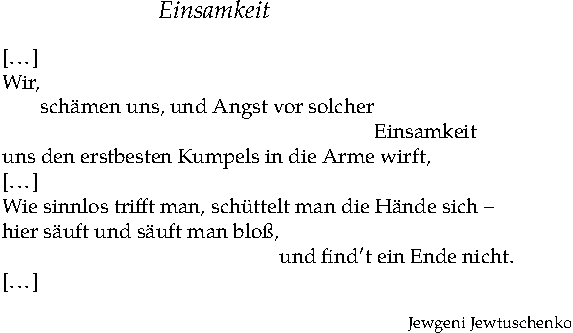
\includegraphics{Roemer-Beispiel3-crop}
\end{center}

Mit der Umgebung \texttt{altverse} können individuell gestaltete Strophen gesetzt werden; sie hat den Effekt, dass z.\,B. bei den paarweise 
strukturierten
Strophen die 2., 4. etc. Zeile um die Länge \verb|\vgap| einrückt.
Als Alternative wird für die \texttt{verse}-Umgebung der Einschluss einzelner
Verse in die \texttt{patverse}-Umgebung angeboten.

\begin{center}
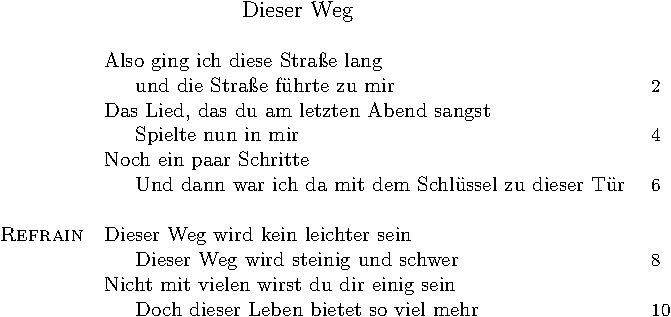
\includegraphics{Roemer-Beispiel-crop}
\end{center}

\begin{lstlisting}
\documentclass[ngerman,a4paper,article]{memoir}
[...]
\settowidth{\versewidth}{Das Lied, das du am letzten Abend sangst}
\PoemTitle*{Dieser Weg}
\begin{verse}[\versewidth]
\linenumberfrequency{2}
\begin{altverse}
  Also ging ich diese Straße lang\\
  und die Straße führte zu mir\\
  Das Lied, das du am letzten Abend sangst\\
  Spielte nun in mir\\
  Noch ein paar Schritte\\
  Und dann war ich da mit dem Schlüssel zu dieser Tür\\!
\end{altverse}

\begin{altverse}
\flagverse{\textsc{Refrain}\quad} Dieser Weg wird kein leichter sein\\
  Dieser Weg wird steinig und schwer\\
  Nicht mit vielen wirst du dir einig sein\\
  Doch dieser Leben bietet so viel mehr\\
\end{altverse}
\linenumberfrequency{0}
\end{verse}
\end{lstlisting}

Das neue poetrytex-Paket von Sam Whited (Juli 2012) ist primär für das Setzen
von poetischen Anthologien geschaffen worden. Die verse-Umgebung wurde darin
etwas modifiziert und in eine \texttt{poem}-Umgebung umgebaut.


\subsection{Darstellen von Reim, Rhythmus und Metrum}

Klassische Gedichte reimen nach bestimmten Schemata. So nennt man beispielsweise
ein Gedicht aus Vierzeilern Quartett. Wenn sich die ersten und die beiden letzten
Zeilen jeweils beim Aussprechen reimen, wird dies als Paarreim bezeichnet. 
Wenn sich das Ende von Verszeilen reimt, ist dies ein Endreim, den es wieder in
verschiedenen Ausprägungen gibt. Veranschaulicht wird dies in der Regel mit
Kleinbuchstaben:

\begin{tabular}{cl}
aabb & Paarreim \\
abab & Kreuzreim \\
abba & umarmender Reim \\
\ldots & \ldots \\
\end{tabular}

Rhythmus und Metrum werden auch Versmaß genannt. Die regelmäßige Abfolge von betonten
und unbetonten Silben ist der Rhythmus, der in der lyrischen Sprache nach einem sich 
wiederholenden Takt (Metrum) aufgebaut sein kann. Eine metrisch gebundene Verszeile 
umfasst mehrere Takte und wird damit als zwei-, drei- oder vierhebig bezeichnet. Man
unterscheidet traditionell nach den Metren verschiedene Rhythmen in den Wortsilben:
den Jambus (unbetont, betont) et cetera. Um mehr Übersichtlichkeit bei der Vermittlung und
Bestimmung des Versmaßes zu bekommen wird die Abfolge von Hebungen und Senkungen auch
graphisch dargestellt. Das übliche Modell nimmt dafür den Backslash (\verb|\|) für eine 
Hebung und "`ein kleines breites U"' ($\cup$) für die Senkung \cite[S.\,17]{Neuhaus}.

Beispielsweise wurde der Daktylus, der schon in der griechischen Ilias Verwendung fand,
während der Klassikepoche in der deutschen Verslehre als Abfolge einer 
betonten und zweier unbetonten Silben definiert.

\begin{tabular}{ll}
betont - unbetont - unbetont: &  \verb|\| $\cup$ $\cup$ \\
\end{tabular}

\begin{lstlisting}
 \verb|\| $\cup$ $\cup$ 
\end{lstlisting}

Um sich die Arbeit etwas zu erleichtern, ist es sinnvoll, Befehle zu definieren.
Es dürfen dafür aber keine Befehle genommen werden, die es schon gibt:
\begin{lstlisting}
\usepackage{xspace}

\newcommand\He{\textbackslash\xspace}%  Hebung
\newcommand\Se{$\cup$\xspace}%  Senkung 
\end{lstlisting}

Der Daktylus tritt in dem folgenden Beispiel auf:

\poemtitle{\textbf{Wür}de der \textbf{Frau}en}
\settowidth{\versewidth}{Ehret die Frauen! sie flechten und weben}
 \poemlines{1} 
\begin{verse}[\versewidth]
\textbf{Eh}ret die \textbf{Frau}en! sie \textbf{flech}ten und \textbf{we}ben\\
\textbf{Himm}lische \textbf{Ro}sen ins \textbf{ir}dische \textbf{Le}ben,\\
\textbf{Flech}ten der \textbf{Lie}be be\textbf{glüc}kendes \textbf{Band},\\
\textbf{Und} in der \textbf{Gra}zie \textbf{züch}tigem \textbf{Schlei}er\\
\textbf{Näh}ren sie \textbf{wach}sam das \textbf{e}wige \textbf{Feu}er\\
\textbf{Schö}ner Ge\textbf{füh}le mit \textbf{hei}liger \textbf{Hand}.\\
\end{verse}
\attrib{Friedrich Schiller}

Das Schema dazu:

\begin{center}

\begin{tabular}{@{}clc@{}}
Vers & Metrum & Reim \\ 
\hline 
  & \He\Se \Se \He\Se \\
1 & \He\Se \Se  \He\Se \Se \He\Se \Se \He\Se  & a\\
2 & \He\Se\Se \He\Se \Se \He\Se\Se \He\Se  & a\\
3 & \He\Se \Se \He\Se \Se\He\Se\Se \He & b\\
4 & \He \Se \Se \He\Se \He\Se\Se \He\Se & c\\
5 & \He\Se \Se \He\Se \Se \He\Se\Se \He\Se & c\\
6 & \He\Se \Se\He\Se \Se \He\Se\Se \He & b\\
\end{tabular}

\end{center}

\begin{lstlisting}
\begin{tabular}{@{}clc@{}}
Vers & Metrum & Reim \\ 
\hline 
 & \He\Se \Se \He\Se \\
1 & \He\Se \Se  \He\Se \Se \He\Se \Se \He\Se  & a\\
2 & \He\Se\Se \He\Se \Se \He\Se\Se \He\Se  & a\\
3 & \He\Se \Se \He\Se \Se\He\Se\Se \He & b\\
4 & \He \Se \Se \He\Se \He\Se\Se \He\Se & c\\
5 & \He\Se \Se \He\Se \Se \He\Se\Se \He\Se & d\\
6 & \He\Se \Se\He\Se \Se \He\Se\Se \He & d\\
\end{tabular}
\end{lstlisting}


Wie zu sehen ist, unterscheiden sich die Verse bei der Betonung der letzten 
Silbe; ist die letzte Silbe im Vers betont, liegt eine männliche, ist sie unbetont
eine weibliche Kadenz
vor. Der Titel, Vers 1, 2, 4, 5 haben weibliche und Vers 3 und 6 haben 
männliche Kadenz.

Wenn man sehen will, wie sich die Hebungen und Senkungen auf die
einzelnen Wörter verteilen, kann der Wortzwischenraum beispielsweise
durch einen Unterstrich markiert werden. Damit keine uneinheitlichen Abstände 
um den Unterstrich entstehen, kann man ein Makro für
den Wortzwischenraum (\verb|Zr|) verwenden:

\verb|\newcommand*{\Zr}{\unskip\textunderscore}|

Würde der Frauen: \He\Se\Zr\Se\Zr\He\Se =\verb|\He\Se\Zr\Se\Zr\He\Se|

%\He\Se\_\Se\_\He\Se \quad = \verb|\He\Se\_\Se\_\He\Se| 


Es ist auch möglich komplexe "`Bausteine"' zu definieren. Beispielsweise
\verb|\daktylus|: \daktylus{} (Daktylus) oder \verb|\anapaest| (Anapäst) 
\anapaest.

\begin{lstlisting}
\newcommand\daktylus{$\textbackslash\cup\cup$\xspace} 
\newcommand\anapaest{$\cup\cup\textbackslash$\xspace} 
\end{lstlisting}

\small
\begin{thebibliography}{1000}
\bibitem
{Neuhaus} Stefan Neuhaus:
\textsl{Grundriss der Literaturwissenschaft}. 
A. Francke Verlag: Tübingen und Basel, 3. überarbeitete und erweiterte Auf\/lage, 
2009.

\bibitem
{Svoboda} Atze Svoboda:
\textsl{Was gesagt werden muss}.
In: Eulenspiegel, Heft 5/2012, S.\,14.

\bibitem
{Willberg} Hans Peter Willberg /Friedrich Forsman:
\textsl{Lesetypografie.}
Verlag Hermann Schmidt: Mainz 2010.

\bibitem
{wilson} Peter R. Wilson/Lars Madsen:
\textsl{The Memoir Class for Configurable Typesetting. User Guide.}
The Herries Press, Normandy Park, WA 2011.
\url{macros/latex/contrib/memoir/memman.pdf}.

\bibitem
{Wilson} Peter R. Wilson:
\textsl{Typesetting simple verse with \LaTeX }. 2004.
\url{macros/latex/contrib/verse/verse.pdf}
\end{thebibliography}

%\end{document}



%\end{document}

	

\section{Dramen}
\autor{Thomas H. Meyer}

\paket{covington}
\paket{dramatist}
\footcite[xxx]{lesetypografie}




%% lfgw: 2.21 Linguistische Beispiele

%% !TEX root = lfgw.tex

\RequirePackage{iftex}
\RequireLuaTeX
\RequirePackage{luatex85}

\documentclass[%
   ibycus,polutonikogreek,english,french,latin,ngerman,%global definiert!
   %%%draft=false,%
   fontsize=11pt,%
   paper=17cm:24cm,%
   DIV=13,%
   listof=totoc,%
   bibliography=totoc,%
   pagesize%
   ]{scrbook}

\KOMAoption{bibliography}{leveldown}

\usepackage{yfonts}
\usepackage{textgreek}
\usepackage{cjhebrew}[2017/03/06]
\usepackage{amsmath,amssymb} % für forrest
%%%\usepackage{textcomp}
\usepackage{unicode-math}
\usepackage{fontspec}
\defaultfontfeatures{Ligatures=TeX,Scale=MatchLowercase}
%\newfontfamily\GFSDidot{GFS Didot}
\newcommand\gkk[1]{%{\GFSDidot
#1}

\usepackage[]{babel}
%\usepackage[ngerman,noftligs]{selnolig}
%%%\setmainfont{Libertinus Serif} %reicht auch, unten evtl. besser wegen SB
\setmainfont{libertinusserif}[
   Extension = {.otf},
   UprightFont = {*-regular}, ItalicFont = {*-italic},
   BoldFont = {*-bold}, BoldItalicFont = {*-bolditalic},%
   FontFace = {sb}{\updefault}{*-semibold},%
   FontFace = {sb}{it}{*-semibolditalic}]%
\setsansfont{Libertinus Sans}
\setmonofont[Scale=MatchLowercase,FakeStretch=0.85]{DejaVu Sans}%das wird für Griechisch in Codebeispielen gebraucht
\setmathfont{Libertinus Math}
\makeatletter
\newcommand*\sustyle{\addfontfeatures{VerticalPosition=Superior}}
\DeclareTextFontCommand{\textsu}{\sustyle}
\def\@makefnmark{\hbox{\sustyle\@thefnmark}}
\makeatother
\DeclareTextCommandDefault{\textborn}{{\char"002A}}
\DeclareTextCommandDefault{\textdied}{{\char"2020}}
\usepackage[% microtype
   final,%
   tracking=smallcaps,%
   expansion=alltext,%
   protrusion=true%
   ]{microtype}%
\SetTracking{encoding=*,shape=sc}{50}%
\UseMicrotypeSet[protrusion]{basicmath} % disable protrusion for tt fonts

\usepackage[headsepline]{scrlayer-scrpage}
\clearscrheadfoot
\ihead{\headmark}
\ohead{\pagemark}
\pagestyle{scrheadings}

\usepackage[autostyle]{csquotes}
\usepackage[newcommands]{ragged2e}

\usepackage{graphicx}
\graphicspath{{bilder/}}

\usepackage{grffile}
\usepackage[a4,center,cross]{crop}

\usepackage{listings}
\lstdefinestyle{listinglfgw}{%
  inputencoding=utf8,
  extendedchars=true,
  language=[LaTeX]{TeX},
  numbers=left, 
  %stepnumber=3,
  numbersep=5pt, 
  numberfirstline=false,  
  numberstyle=\tiny\textsf,
  basicstyle=\ttfamily\footnotesize,
  keywordstyle=\bfseries,%
  texcsstyle=*\ttfamily\footnotesize\bfseries,%
  %frame=tlrb,
  breaklines=true,
  breakatwhitespace=true,
  breakindent=5pt,
  %postbreak=\mbox{$\hookrightarrow$},
  escapeinside={*@}{@*},
  %showstringspace=false, 
  captionpos=b,
  upquote=true,
  %%%classoffset=0,
  morekeywords={%
  %a
  addbibresource,addplot,Afootnote,alteSeite,autocite,autopar,answerline,alertblock,
  %b
  beginnumbering,Bfootnote,biblerefformat,biblerefmap,biblerefstyle,bonuspointpoints,bibleref,block,
  %c
  Cfootnote,chapter,chbpword,chpword,chpgword,chqword,chsword,chtword,citeauthor,cites,citetitle,columnrulewidth,Columns,columnsposition, center,
  chronology,columns,
  %d
  draw,dictum,deffootnote,deffootnote,description,
  %e
  edtext,endnumbering,enquote,enumi,example,exampleblock,
  %f
  firstlinenum,firstlinenumR,firstpageheadrule,footcite,footcites,footfullcite,fullcite,fillwithgrid,fillwithlines,fillwithdottedlines,Forest,Forest*,
  footnotemargin,fillwithlines, fillwithgrid,
  %h
  hpword,hqword,hsword,htword,hypertarget,hyperlink,hideallsubsection,
  %i
  includegraphics,includeonlyframes,ibibleref,invisible,
  %l
  Lcolwidth,ledsidenote,lemma,linenumincrement,linenumincrementR,
  %m
  msdata,mode,maketitle,multifootsep,
  %n
  newfontface,newfontfamily,node,
  %o
  only,onslide,
  %p
  Pages,parencite,parencites,part,pend,pibibleverse,pbibleverse,pointpoints,printbibheading,printbibliography,printindex,pstart,pgfimage,pgfusepath,
  pgfplothandlerlineto,pgfplotsset,pgfplotxyfile,pbibleref,pibibleref,pgf-pie,plain,
  %q
  quell,question,quote,quotaion,
  %r
  Rcolwidth,reledmac,
  %s
 selectlanguage,setlength,setmainfont,setmonofont,setmsdatalabel,setromanfont,setsansfont,smartcite,smartcites,solutiontitle,setbeamerfont,setbeamercovered,subsection,subsection*,subsubsection,subtitle,solution,solutionorgrid,
  %t
  text,textborn,textcite,textcites,textdelta,textDelta,textdied,texteuro,textgamma,textGamma,textmarried,textsubscript,thealteSeite,tableofcontents,th,TH,
  textalpha, textbeta, textgamma, textdelta, textepsilon, textzeta, texteta, texttheta, textiota, textkappa, textlambda, textmu, textnu,
  textxi, textomikron, textpi, textrho, textsigma, texttau, textupsilon, textphi, textchi,  textpsi, textomega,
  textAlpha, textBeta, textGamma, textDelta, textEpsilon, textZeta, textEta, textTheta, textIota, textKappa, textLambda, textMu, textNu,
  textXi, textOmikron, textPi, textRho, textSigma, textTau, textUpsilon, textPhi, textChi,  textPsi, textOmega, twocolumn,
  %u
  usetheme,usecolortheme,usebackgroundtemplate,useforestlibrary,usepackage,usetikzlibrary,
  %v
  vari,verse,
  %x
  Xafternumber,Xarrangement,Xlemmaseparator,Xinplaceoflemmaseparator,Xinplaceofnumber,Xnonbreakableafternumber,Xnotenumfont,Xnumberonlyfirstinline,Xnumberonlyfirstintwolines,Xsymlinenum,Xtwolines,Xtwolinesbutnotmore,Xtxtbeforenotes
  },   
  literate=
  {á}{{\'a}}1 {é}{{\'e}}1 {í}{{\'i}}1 {ó}{{\'o}}1 {ú}{{\'u}}1
  {Á}{{\'A}}1 {É}{{\'E}}1 {Í}{{\'I}}1 {Ó}{{\'O}}1 {Ú}{{\'U}}1
  {à}{{\`a}}1 {è}{{\`e}}1 {ì}{{\`i}}1 {ò}{{\`o}}1 {ù}{{\`u}}1
  {À}{{\`A}}1 {È}{{\'E}}1 {Ì}{{\`I}}1 {Ò}{{\`O}}1 {Ù}{{\`U}}1
  {ä}{{\"a}}1 {ë}{{\"e}}1 {ï}{{\"i}}1 {ö}{{\"o}}1 {ü}{{\"u}}1
  {Ä}{{\"A}}1 {Ë}{{\"E}}1 {Ï}{{\"I}}1 {Ö}{{\"O}}1 {Ü}{{\"U}}1
  {â}{{\^a}}1 {ê}{{\^e}}1 {î}{{\^i}}1 {ô}{{\^o}}1 {û}{{\^u}}1
  {Â}{{\^A}}1 {Ê}{{\^E}}1 {Î}{{\^I}}1 {Ô}{{\^O}}1 {Û}{{\^U}}1
  {œ}{{\oe}}1 {Œ}{{\OE}}1 {æ}{{\ae}}1 {Æ}{{\AE}}1 {ß}{{\ss}}1
  {ç}{{\c c}}1 {Ç}{{\c C}}1 {ø}{{\o}}1 {å}{{\r a}}1 {Å}{{\r A}}1
  {€}{{\EUR}}1 {£}{{\pounds}}1
}
\lstset{style=listinglfgw}
  
\usepackage[% tcolorbox
  skins,%
  listings,%
  breakable,%
]{tcolorbox}
\tcbset{%
lfgwstyle/.style={%
    before skip=\baselineskip,
    boxrule=0pt,
    %bottomrule=2pt,
    %toprule=2pt,
    %colframe=black,
    colback=black!5,
    coltitle=white,
    bicolor,
    sharp corners,
    colbacklower=white,
    fonttitle=\sffamily\bfseries,
    breakable,
    %label=#1,
}}


\newtcblisting[auto counter,number within=chapter]{lfgwexample}[1]{%
    lfgwstyle,
    fontupper=\small\ttfamily,
    sidebyside,
    listing and text,
    title={Beispiel \thetcbcounter},
    listing options={style=listinglfgw},
    #1,
%text and listing,
}

\newtcblisting[use counter from=lfgwexample,number within=chapter]{lfgwcode}[1]{%
    lfgwstyle,
    fontupper=\small\ttfamily,
    listing only,
    title={Beispiel \thetcbcounter},
    listing options={style=listinglfgw},
    #1,
}

\newtcblisting[use counter from=lfgwexample,number within=chapter]{lfgwprint}[1]{%
    fontupper=\small,
    lfgwstyle,
    text only,
    title={Beispiel \thetcbcounter},
    listing options={style=listinglfgw},
    #1,
}


\usepackage{showexpl}
%\lstset{explpreset={escapeinside={*@}{@*}}}

\usepackage[pagewise]{lineno}
\usepackage{sidenotes}
\usepackage{multicol}
% Für den Abschnitt über Konstituentenanylyse von C. Römer:
\usepackage[linguistics]{forest}
\forestapplylibrarydefaults{linguistics,edges}
\useforestlibrary{edges}
\makeatletter
\let\pgfmathModX=\pgfmathMod@
\usepackage{pgfplots}%
\pgfplotsset{compat=1.14}
\let\pgfmathMod@=\pgfmathModX
\makeatother
%http://tex.stackexchange.com/questions/328972/presence-of-pgfplots-package-breaks-forest-environment-%w-folder-option-en/329015

% Pakete im Bereich Kapitel 3 - Diagramme zeichnen
\usepackage{tikz}
\usepackage[all]{genealogytree}
\usepackage{chronology}
\usepackage{pgf-pie}
\usetikzlibrary{pgfplots.dateplot}
\usetikzlibrary{mindmap}

\deffootnote[1.5em]{1.5em}{1.5em}{\makebox[1.5em][l]{{\fontseries{sb}\selectfont\thefootnotemark\ }}}

\usepackage{enumitem}			% for simple list modifications
\setlist{leftmargin=*,before=\setlength{\rightmargin}{\leftmargin}}

%\usepackage{parallel}


%- Für Lyrik-Satz, Christine Römer:
\usepackage{verse}
\newcommand\He{\textbackslash\xspace}
\newcommand\Se{$\cup$\xspace} 
\newcommand*{\Zr}{\unskip\textunderscore}
\newcommand\daktylus{\textbackslash$\cup\cup$\xspace} 
\newcommand\anapaest{$\cup\cup$\textbackslash\xspace}

% ------------
\usepackage{runic}
\usepackage{hieroglf}
\usepackage[normalem]{ulem} %%% MS: Wofür? Unterstreichungen sollten vermieden werden! LCB: kann \xout
%\usepackage{letterspace} %%% MS: Wofür. Besser direkt \textls aus dem Microtypepaket
%% ------------------------------------------------------------------------
%%   This is a stand-alone version that only provides the letterspacing
%%   commands. Do not use this package together with the `microtype' package.
%%   Please refer to section 7 of the `microtype' documentation.
%% ------------------------------------------------------------------------ 
\usepackage[hyphens]{url}
\usepackage{hologo}
\usepackage{philex}
\def\fg{}
\usepackage{siunitx} %Supreme typesetting of units
%\sisetup{%
%    tight-spacing=true, %
%    %math-rm=\mathsf, 
%    %		text-rm=\sffamily,
%    detect-all, %Zahlen werden in der aktuellen Schrift angezeigt
%    detect-family,
%    exponent-to-prefix  	= true,%
%    round-mode          	= places,% 
%    round-precision     	= 2,%
%    group-minimum-digits 	= 4, % Für "Tausenderpunkt" --> 1.234 anstatt 1234
%    group-separator			={.},% für "12.345" statt "12 345"
%    %  scientific-notation = engineering, % Use multiples of 3 as exponent
%    locale					=DE, % Typeset numbers and units the German way
%    range-phrase 			={$\times$},%
%    %		zero-decimal-to-integer,%aus "2.0" wird "2"
%    range-units				=single,  % --> 2 x 2 m, - auskommentieren für 2 m x 2 m
%    %%%---------
%%    unit-color=myred,
%}

\usepackage[german]{keystroke}% Computer-Tastatur-Tasten in Anweisungs-Texte zu setzen (z.B. \Shift, \Ctrl, \Spacebar).

\usepackage{imakeidx}
\indexsetup{level = \subsection*, toclevel = subsection, noclearpage, headers = {\indexname}{\indexname}}
\makeindex[                title = {Allgemeiner Index}]
\makeindex[name = pakete,  title = {Verzeichnis der Paketnamen}]
\usepackage[% biblatex
   style=authoryear,  
%  style=historische-zeitschrift, % das am liebsten - aber der geht (bei mir?) nicht!
%  pageref=true,
	backend=biber
	]{biblatex}
\addbibresource{lfgw-bibliographie.bib}
%%%\defbibheading{bibliography}{\addchap{#1}} %%%Besser bei \addchap bleiben

\usepackage{fancyvrb}
\makeatletter
\usepackage[% reledmac
   series={A,B,C},%nur die Apparate A B C aktivieren
   noend,%keine Endotenapparate
   noeledsec%keine eledsections et al.
   %noledgroup%keine ledgroups -- das muss hier auskommentiert werden, damit die minipages funktionieren!
]{reledmac}%
\@ifpackagelater{reledmac}{2017/03/20}{%
   % Package is new enough
}{%
\PackageError{reledmac}{Es wird reledmac >= 2.18.1 benötigt.}%
}
\makeatother
\usepackage{reledpar}

\usepackage{varioref}
\usepackage{hyperxmp}
\usepackage{hyperref}
\hypersetup{					% setup the hyperref-package options
	pdftitle={LaTeX für Geisteswissenschaftler},	% 	- title (PDF meta)
	pdfsubject={Handbuch},% 	- subject (PDF meta)
	pdfauthor={varia},	% 	- author (PDF meta)
	pdfauthortitle={},
	pdfcopyright={Copyright (c) \the\year\. All rights reserved.},
	pdfhighlight=/N,
	pdfdisplaydoctitle=true,
	pdfdate={\the\year-\the\month-\the\day}
	pdflang={de},
   pdfencoding=unicode,   % Sorgt für korrekte Umlaute in den pdf-Lesezeichen - thm
	pdfcaptionwriter={varia},
	pdfkeywords={{LaTeX}, {Geisteswissenschaften}},
	pdfproducer={LuaLaTeX},
	pdflicenseurl={http://creativecommons.org/licenses/by-nc-nd/4.0/},
	plainpages=false,			% 	- 
   colorlinks   = true, %Colours links instead of ugly boxes
   urlcolor     =  blue!50!black, %Colour for external hyperlinks
   linkcolor    = blue, %Colour of internal links
   citecolor   = green!50!black, %Colour of citations
   linktoc=page,
  	pdfborder={0 0 0},			% 	-
	breaklinks=true,			% 	- allow line break inside links
 %   bookmarks=true,
	bookmarksnumbered=true,		%
	bookmarksopenlevel=2,
	bookmarksopen=true,		%
   bookmarksdepth=3,
   pdfdisplaydoctitle,
	final=true	% = true, nur bei web-Dokument!! (wichtig!!)
}
\usepackage{bookmark}%advanced bookmarks
\usepackage[% cleveref
  sort,
  nameinlink
  ]{cleveref}%nach hyperref laden

\crefname{tcb@cnt@lfgwexample}{Beispiel}{Beispiele}
\addto\captionsngerman{%
    \crefformat{lfgwexample}{#2Beispiel\,#1#3}%
    \crefformat{lfgwcode}{#2Beispiel\,#1#3}%
    \crefformat{lfgwprint}{#2Beispiel\,#1#3}%
}

\setkomafont{pagehead}{\normalcolor\normalfont\small\upshape}
\setkomafont{pagenumber}{\normalcolor\normalfont\normalsize\bfseries}

\renewcommand*{\glqq}{\textquotedblleft}
\renewcommand*{\grqq}{\quotedblbase}

\providecommand*{\reledmac}{\mbox{\Package{reledmac}}\xspace}

\providecommand*{\LaTeXTeX}{\hologo{(La)TeX}}
\providecommand*{\AmSLaTeX}{\hologo{AmSLaTeX}}
\providecommand*{\AmSTeX}{\hologo{AmSTeX}}
\providecommand*{\biber}{\hologo{biber}}
\providecommand*{\BibTeX}{\hologo{BibTeX}}
\providecommand*{\BibTeXacht}{\hologo{BibTeX8}}
\providecommand*{\ConTeXt}{\hologo{ConTeXt}}
\let\context\ConTeXt
\providecommand*{\emTeX}{\hologo{emTeX}}
\providecommand*{\eTeX}{\hologo{eTeX}}
\providecommand*{\ExTeX}{\hologo{ExTeX}}
\providecommand*{\HanTheThanh}{\hologo{HanTheThanh}}
\providecommand*{\iniTeX}{\hologo{iniTeX}}
\providecommand*{\KOMAScript}{\hologo{KOMAScript}}
\providecommand*{\LaTeX}{\hologo{LaTeX}}
\providecommand*{\LaTeXe}{\hologo{LaTeX2e}}
\providecommand*{\LaTeXIII}{\hologo{LaTeX3}}
\providecommand*{\LaTeXML}{\hologo{LaTeXML}}
\providecommand*{\LuaLaTeX}{\hologo{LuaLaTeX}}
\let\lualatex\LuaLaTeX
\providecommand*{\LuaTeX}{\hologo{LuaTeX}}
\let\luatex\LuaTeX
\providecommand*{\LyX}{\hologo{LyX}}
\providecommand*{\METAFONT}{\hologo{METAFONT}}
\let\MF\METAFONT
\providecommand*{\MetaFun}{\hologo{MetaFun}}
\providecommand*{\METAPOST}{\hologo{METAPOST}}
\providecommand*{\MetaPost}{\hologo{MetaPost}}
\let\MP\METAPOST
\providecommand*{\MiKTeX}{\hologo{MiKTeX}}
\providecommand*{\NTS}{\hologo{NTS}}
\providecommand*{\OzMF}{\hologo{OzMF}}
\providecommand*{\OzMP}{\hologo{OzMP}}
\providecommand*{\OzTeX}{\hologo{OzTeX}}
\providecommand*{\OzTtH}{\hologo{OzTth}}
\providecommand*{\PCTeX}{\hologo{PCTeX}}
\providecommand*{\pdfTeX}{\hologo{pdfTeX}}
\let\pdftex\pdfTeX
\providecommand*{\pdfLaTeX}{\hologo{pdfLaTeX}}
\let\pdflatex\pdfLaTeX
\providecommand*{\PiC}{\hologo{PiC}}
\providecommand*{\PiCTeX}{\hologo{PiCTeX}}
\providecommand*{\plainTeX}{\hologo{plainTeX}}
\providecommand*{\SageTeX}{\hologo{SageTeX}}
\providecommand*{\SLiTeX}{\hologo{SLiTeX}}
\providecommand*{\teTeX}{\hologo{teTeX}}
\providecommand*{\TeXivht}{\hologo{TeX4ht}}
\providecommand*{\TTH}{\hologo{TTH}}
\providecommand*{\virTeX}{\hologo{virTeX}}
\providecommand*{\VTeX}{\hologo{VTeX}}
\providecommand*{\XeLaTeX}{\hologo{XeLaTeX}}
\providecommand*{\XeTeX}{\hologo{XeTeX}}
%%
\newcommand\BibTool{\textsc{Bib\hskip-.1em
      T\hskip-.15emo\hskip-.05emo\hskip-.05eml}\xspace}
\providecommand*{\TikZ}{\textsf{Ti\textit{k}Z}}
%\providecommand*{\pgf/tikz}{\textsf{pgf/Ti\textit{k}Z}}
\def\pgf/tikz{\textsf{pgf/Ti\textit{k}Z}}
\providecommand*{\ALEPH}{\ensuremath{\aleph}}

\providecommand\eV{e.V\kern-0.18em\@ifnextchar.{}{.}\kern0.18em}
\providecommand\dante{\mbox{DANTE~\eV}}
\providecommand\Dante{DANTE,
   Deutschsprachige Anwendervereinigung \TeX~\eV}
\providecommand\DTK{Die \TeX\-ni\-sche Ko\-m{\"o}\-die}
\providecommand\PS{Post\-Script}
\providecommand\TUG{\TeX{} Users Group}
\providecommand\TUGboat{\textsl{TUGboat}}
\let\DANTE\dantelogo
\providecommand*{\TeXLive}{\TeX{}Live}

\def\BibLaTeX{Bib\hologo{LaTeX}}
\let\biblatex\BibLaTeX
\providecommand*{\CTAN}{\texttt{CTAN}\xspace}

\providecommand*{\prog}[1]{\texttt{#1}}
\let\Program\prog

\providerobustcmd*{\paket}[2][]{\textsf{#2}\index[pakete]{\if$#1$#2\else#1\fi}}
\let\Package\paket%zwecks kompatibilität mit DTK
\let\Paket\paket
\newcommand*{\opt}[1]{\texttt{#1}}
\newcommand*{\file}[1]{\texttt{#1}}
\newcommand*{\env}[1]{\texttt{#1}}

\makeatletter
\DeclareRobustCommand\cs[1]{\texttt{\bfseries\char`\\#1}}
\DeclareRobustCommand\meta[1]{%
   \ensuremath\langle
   \ifmmode \expandafter \nfss@text \fi
   {%
      \meta@font@select
      \edef\meta@hyphen@restore
      {\hyphenchar\the\font\the\hyphenchar\font}%
      \hyphenchar\font\m@ne
      \language\l@nohyphenation
      #1\/%
      \meta@hyphen@restore
   }\ensuremath\rangle
}
\def\marg{\@ifstar{\@@marg}{\@marg}}
\providecommand\@marg[1]{%
   {\ttfamily\mdseries\char`\{}\meta{#1}{\ttfamily\mdseries\char`\}}}
\providecommand\@@marg[1]{%
   {\ttfamily\mdseries\char`\{}{\mdseries #1}{\ttfamily\mdseries\char`\}}}
\def\oarg{\@ifstar{\@@oarg}{\@oarg}}
\providecommand\@oarg[1]{%
   {\ttfamily\mdseries[}\meta{#1}{\ttfamily\mdseries]}}
\providecommand\@@oarg[1]{%
   {\ttfamily\mdseries[}{#1}{\ttfamily\mdseries]}}
\providecommand\parg[1]{%
   {\ttfamily\mdseries(}\meta{#1}{\ttfamily\mdseries)}}
\def\meta@font@select{\itshape\mdseries}
\makeatother

\tolerance 1414
\hbadness 1414
\emergencystretch 1.5em
\hfuzz 0.3pt
\widowpenalty=10000
\displaywidowpenalty=10000
\clubpenalty=5000
\interfootnotelinepenalty=9999
\brokenpenalty=2000
\vfuzz \hfuzz
%%%\raggedbottom


% Autorkennung:   Wie soll's aussehen?
\providecommand{\autor}[1]{\hfill\textbf{#1}}

\endinput


%\begin{document}

\section{Linguistische Beispiele}
\autor{Christine Römer}

\subsection{Belege einfügen mit \texttt{philex}}
\label{belege} \index{Belege}
\author{Christine Römer}

Die neuerliche Hinwendung der Linguistik zur Empirie hat es mit sich gebracht, dass eigentlich keine Feststellung ohne reale sprachliche Belege
auskommt. Dies geschieht in der Regel durch eingezogene, durchnummerierte Belege, die mit Grammatikalitätsurteilen in Form von festgelegten Abkürzungen (beispielsweise * =ungrammatisch, ? = fraglich) versehen werden können.
Im laufenden Text wird sich dann auf diese Beispiele bezogen. Im Unterschied zu mathematischen Texten steht die Beispielnummer links und nicht rechts.

Mit dem neueren Paket \paket{philex} ist dies einfach zu bewerkstelligen.
Es wird mit \verb|\usepackage[<package options>]{philex}|\footnote{Paketdokumentation: texdoc philex} in die Präambel eingebunden, es lädt dabei automatisch \paket{linguex}, auf dem es aufbaut, sowie \paket{xspace} und \paket{cgloss4e}. Die möglichen Paketoptionen sind \texttt{hyper, draft, oldpunkt}.

Der Befehl für die Basisumgebung ist  \verb|lb{}{}|, er hat also
zwei obligatorische Argumente: Das erste ist für das Label, den Anker und das zweite für den Inhalt (Beispiel~\ref{example:1}):

\begin{lfgwexample}{label={example:1}}
So wurde in der SDZ am 21.02.\,2017 der Neologismus \emph{Bierpreispremse} geprägt (siehe Beispiel \ref{bier}).

\lb{bier}{Die Bierpreisbremse soll im Zuge einer kompletten Neuorganisation der Wiesn-Finanzierung umgesetzt werden .}

und von weiteren Preisbremsen wird geschrieben, bspw. bei Reuters am 11.04.\,2016 von einer \enquote{Arznei-Preisbremse} (siehe \ref{arznei}).

\lb{arznei}{Pharmaindustrie kritisiert Pläne für Arznei-Preisbremse} 

\end{lfgwexample}

An Stelle einer Nummer kann der Zähler auch auf Buchstaben o.\,ä. mit dem Befehl \verb|\bpaformat{1}{(Beleg~}{)}| umgestellt werden
(wie in \ref{example:2}):

\begin{lfgwexample}{label={example:2}}
\bpaformat{1}{(Beleg~}{)}
\lbpa{kno}{Mietpreisbremse}
\lbpa{hu}{Preisbremse im Grundstückverkauf}
\end{lfgwexample}

Untergliederungen bei den Belegen sind auch möglich (wie in \ref{example:3}/\ref{example:4}):

\begin{lfgwcode}{label={example:3}}
\lbp{clauses}{AdvP}{Adverbiengebrauch:
\lba{first}{Die erste Klasse
\lba{firstnew}{adverbiell: Sie wohnt \emph{hier}.}
\lbb{lastnew}{prädikativ: Sie ist \emph{hier}.}
\lbz{attr}{attributiv: Die \emph{dort} wohnt hier.}}
\lbb{second}{Die zweite Klasse
\lba{adverb}{nur adverbial: Sie liest \emph{gern}.}}}
\end{lfgwcode}

\begin{lfgwprint}{label={example:4}}
\lbp{clauses}{AdvP}{Adverbiengebrauch:
\lba{first}{Die erste Klasse
\lba{firstnew}{adverbiell: Sie wohnt \emph{hier}.}
\lbb{lastnew}{prädikativ: Sie ist \emph{hier}.}
\lbz{attr}{attributiv: Die \emph{dort} wohnt hier.}}
\lbb{second}{Die zweite Klasse
\lba{adverb}{nur adverbial: Sie liest \emph{gern}.}}}
\end{lfgwprint}


Grammatikalitätsurteile mit dem Befehl \verb|\oddity{ }| einfügen (wie in \ref{example:5}/\ref{example:6}):

\begin{lfgwcode}{label={example:5}}
Genitiv-s für Eigennamen?
\lb{gram}{
\lba{grama}{\oddity{*}die Entwicklung Friedrich Schiller}
\lbb{gramb}{\oddity{?}die Entwicklung Friedrich Schiller-s}
\lbc{grama}{\oddity{*}die Entwicklung Friedrich Schiller}
}
\end{lfgwcode}

\begin{lfgwprint}{label={example:6}}
Genitiv-s für Eigennamen:
\lb{gram}{
\lba{grama}{\oddity{*}die Entwicklung Friedrich Schiller}
\lbb{gramb}{\oddity{??}die Entwicklung Friedrich Schiller-s}
\lbz{gramz}{\oddity{}die Entwicklung Friedrich Schiller}
}
\end{lfgwprint}

Auch für Glossierungen kann das Paket eingesetzt werden 
(wie in dem Beispiel \ref{example:7}/\ref{example:6} aus der Paketdokumentation):

\begin{lfgwcode}{label={example:7}}
\lb{gloss}{\gll Wenn jemand in die Wüste zieht ... \\
If someone in the desert draws and lives ... \\
\trans ‘if one retreats to the desert and ... ’}
\end{lfgwcode}

\begin{lfgwprint}{label={example:8}}
\lb{gloss}{\gll Wenn jemand in die Wüste zieht ... \\
If someone in the desert draws and lives ... \\
\trans ‘if one retreats to the desert and ... ’}
\end{lfgwprint}



%\end{document}




\section{Querverweise im Text}
\autor{Thomas Hilarius Meyer}

%Philipp meint: Lukas hatte vorgeschlagen, zumindest /auch/ das cleveref-Paket hier vorzustellen, das nimmt einem etwas Arbeit ab

\lstinline/\label{key}/

\lstinline/\ref{key}/

\lstinline/\pageref{key}/


\section{Eigene Kommandos und Umgebungen definieren}
\label{makros}

\minisec{Kommandos}

\minisec{Umgebungen}
